% Anonymous ICLR 2027 manuscript. Build with ./build.sh. Numerical tables are generated.
\documentclass{article}
\usepackage{iclr2027_conference,times}

\usepackage[utf8]{inputenc}
\usepackage[T1]{fontenc}
\usepackage{amsmath,amssymb,amsfonts}
\usepackage{graphicx}
\usepackage{booktabs}
\usepackage{multirow}
\usepackage{array}
\usepackage{xcolor}
\usepackage{tikz}
\usetikzlibrary{positioning,arrows.meta,calc,fit,backgrounds,shapes.geometric}
\usepackage{caption}
\captionsetup{font=small,labelfont=bf}
\usepackage{hyperref}
\hypersetup{hidelinks}
\usepackage{url}
\usepackage{microtype}
\usepackage{placeins}
\usepackage{float}
\usepackage{enumitem}
\setlist{nosep,leftmargin=*}

\usepackage{todonotes}
\usepackage{soul}

\graphicspath{{figures/}}
%
% macros.tex -- notation for the NM-ROM methods section.
% Symbol conventions (kept deliberately disjoint from the old submission, which
% overloaded K for both the discrete operator and a latent-adjacent quantity):
%   N  unknowns of the full-order state      k  latent dimension
%   R  spatial bank width (R' used by a query)   M  number of tests
%   N_eq  number of empirical-quadrature nodes

\newcommand{\Real}{\mathbb{R}}
\newcommand{\Nat}{\mathbb{N}}

% --- discrete objects -------------------------------------------------------
\newcommand{\Aop}{K}                    % fixed linear discrete operator
\newcommand{\bank}{G}                   % frozen spatial bank, n x R
\newcommand{\head}{h}            % nonlinear coefficient map, R^k -> R^R
\newcommand{\tests}{P}                  % weak test matrix, M x n
\newcommand{\rowscale}{\Lambda}         % diagonal row scaling
\newcommand{\lift}{u_{g}}               % boundary lift
\newcommand{\bcmask}{\mu}               % boundary mask / vanishing factor
\newcommand{\latent}{z}
\newcommand{\umanifold}{u}

% --- operators and norms ----------------------------------------------------
\newcommand{\jac}[1]{J_{#1}}
\newcommand{\dhead}{J_{h}}
\newcommand{\norm}[1]{\lVert #1 \rVert}
\newcommand{\normF}[1]{\lVert #1 \rVert_{F}}
\newcommand{\inner}[2]{\langle #1, #2 \rangle}
\newcommand{\T}{^{\top}}
\newcommand{\Tr}{\operatorname{tr}}
\newcommand{\diag}{\operatorname{diag}}
\newcommand{\rank}{\operatorname{rank}}
\newcommand{\argmin}{\operatorname*{arg\,min}}

% --- residuals --------------------------------------------------------------
\newcommand{\rfull}{R}                  % full discrete residual
\newcommand{\rweak}{r_{w}}              % weak (projected, row-scaled) residual
\newcommand{\station}[2]{\eta(#1,#2)}   % normalized-gradient stationarity measure

% --- placeholders for generated numbers -------------------------------------
% Every numeric value in this manuscript must come from a generator script that
% reads the run JSONs. \todo marks a slot that the generator has not yet filled.
% \todo now comes from todonotes (line 22); the local definition clashed with it.
\newcommand{\gen}[1]{\todo{pending: #1}}

% Subscripted variants (the base macros already carry a subscript, so
% \head_a / \rweak_n would be a double subscript).
\newcommand{\headc}[1]{h_{#1}}   % one component of the head output
\newcommand{\rweakn}[1]{r_{w,#1}}       % the weak residual of time step #1

%
% GENERATED by paper/gen_tables.py -- do not edit.
% Every prose number in the manuscript is one of these macros.
\newcommand{\nAblBurgersBestFound}{2.5447}
\newcommand{\nAblBurgersFloor}{0.3918}
\newcommand{\nAblBurgersFree}{0.6027}
\newcommand{\nAblBurgersFreeMs}{2417.6}
\newcommand{\nAblBurgersLinear}{56.9296}
\newcommand{\nAblBurgersNeural}{2.5629}
\newcommand{\nAblBurgersNeuralMs}{47.6}
\newcommand{\nAblBurgersPodOneTwentyEight}{10.1198}
\newcommand{\nAblBurgersPodOneTwentyEightMs}{328.3}
\newcommand{\nAblBurgersPodSixteen}{61.6503}
\newcommand{\nAblBurgersQuad}{31.8276}
\newcommand{\nAblBurgersReductionOverFloor}{6.5}
\newcommand{\nAblBurgersSolverGapPp}{0.018}
\newcommand{\nAblPoissonBestFound}{6.0926}
\newcommand{\nAblPoissonDst}{0.0007}
\newcommand{\nAblPoissonDstMs}{4.341}
\newcommand{\nAblPoissonFloor}{2.3148}
\newcommand{\nAblPoissonFree}{2.3274}
\newcommand{\nAblPoissonLinear}{17.2966}
\newcommand{\nAblPoissonNeural}{6.0927}
\newcommand{\nAblPoissonNeuralMs}{5.843}
\newcommand{\nAblPoissonPodOneTwentyEight}{4.3452}
\newcommand{\nAblPoissonPodOneTwentyEightMs}{5.930}
\newcommand{\nAblPoissonPodSixteen}{20.0548}
\newcommand{\nAblPoissonQthirtytwo}{4.6670}
\newcommand{\nAblPoissonQthirtytwoMs}{7.317}
\newcommand{\nAblPoissonQuad}{16.6303}
\newcommand{\nBlockBlockBudgetExits}{0}
\newcommand{\nBlockBlockErr}{2.1489}
\newcommand{\nBlockBlockMs}{619.2}
\newcommand{\nBlockJointBudgetExits}{6}
\newcommand{\nBlockJointErr}{2.1489}
\newcommand{\nBlockJointMs}{1119.7}
\newcommand{\nCgLshapeCgTol}{$10^{-10}$}
\newcommand{\nCgLshapeMeshes}{$64^2$, $128^2$, $256^2$, $512^2$}
\newcommand{\nCgLshapePcgRatioMax}{990.8}
\newcommand{\nCgLshapePcgRatioMin}{3.6}
\newcommand{\nCgLshapeSpeedupMax}{14.9}
\newcommand{\nCgLshapeSpeedupMin}{2.9}
\newcommand{\nCgPoissonCgMsTwoFiftySix}{38.0}
\newcommand{\nCgPoissonDstFasterMax}{4.0}
\newcommand{\nCgPoissonDstFasterMin}{1.3}
\newcommand{\nCgPoissonSpeedupMax}{23.4}
\newcommand{\nCgPoissonSpeedupMin}{3.7}
\newcommand{\nColdCapEightNearest}{6.09}
\newcommand{\nColdCapEightZero}{30.03}
\newcommand{\nColdCapTwelveNearest}{6.09}
\newcommand{\nColdCapTwelveZero}{6.09}
\newcommand{\nColdCapTwoNearest}{6.80}
\newcommand{\nColdCapTwoZero}{91.88}
\newcommand{\nColdConvNearest}{6.09}
\newcommand{\nColdConvZero}{6.09}
\newcommand{\nColdMesh}{1024}
\newcommand{\nColdStarts}{nearest, zero}
\newcommand{\nEqtopBar}{0.116}
\newcommand{\nEqtopBarOrigin}{the held-out $\rho$ of the incumbent $q{=}0$ rule at the state carrying the first-interval penalty, measured in the q-diag cell and adopted as the primary bar in the q-ridge design before any certification job ran; the tight bar was declared before b-eqtop ran}
\newcommand{\nEqtopConfirmedCount}{3}
\newcommand{\nEqtopConfirmedRungs}{0, 16, 32}
\newcommand{\nEqtopCostRatioMax}{0.21}
\newcommand{\nEqtopCostRatioMin}{0.18}
\newcommand{\nEqtopLadderConverged}{yes}
\newcommand{\nEqtopLadderCostSpan}{12.23}
\newcommand{\nEqtopLadderErrSpan}{3.51}
\newcommand{\nEqtopLadderFirstErr}{1.8891}
\newcommand{\nEqtopLadderFirstMs}{59.1}
\newcommand{\nEqtopLadderLastErr}{0.5389}
\newcommand{\nEqtopLadderLastMs}{722.2}
\newcommand{\nEqtopLadderMonotone}{yes}
\newcommand{\nEqtopMarginalCount}{3}
\newcommand{\nEqtopMarginalRungs}{64 (2/6), 128 (4/5), 256 (1/5)}
\newcommand{\nEqtopParentOneTwentyEightRho}{0.1908}
\newcommand{\nEqtopParentTwoFiftySixRho}{0.1678}
\newcommand{\nEqtopPendingJob}{none}
\newcommand{\nEqtopPrimaryOneTwentyEight}{yes}
\newcommand{\nEqtopPrimaryOneTwentyEightM}{2048}
\newcommand{\nEqtopPrimaryOneTwentyEightRho}{0.0669}
\newcommand{\nEqtopPrimaryOneTwentyEightStates}{64}
\newcommand{\nEqtopPrimaryTwoFiftySix}{yes}
\newcommand{\nEqtopPrimaryTwoFiftySixM}{2048}
\newcommand{\nEqtopPrimaryTwoFiftySixRho}{0.1074}
\newcommand{\nEqtopPrimaryTwoFiftySixStates}{64}
\newcommand{\nEqtopQsixtyFourArchivedRho}{0.0531}
\newcommand{\nEqtopQsixtyFourRedrawRho}{0.1220}
\newcommand{\nEqtopSpreadMax}{9.6}
\newcommand{\nEqtopSpreadMin}{1.4}
\newcommand{\nEqtopStaticWorstFit}{1.5e-04}
\newcommand{\nEqtopStaticWorstOverBar}{4.0}
\newcommand{\nEqtopStaticWorstQ}{256}
\newcommand{\nEqtopStaticWorstRho}{0.462}
\newcommand{\nEqtopStatus}{final}
\newcommand{\nEqtopStatusQOneTwentyEight}{marginal (4 of 5 draws pass)}
\newcommand{\nEqtopStatusQSixteen}{confirmed (3 of 3 re-draws)}
\newcommand{\nEqtopStatusQSixtyFour}{marginal (2 of 6 draws pass)}
\newcommand{\nEqtopStatusQThirtyTwo}{confirmed (2 of 2 re-draws)}
\newcommand{\nEqtopStatusQTwoFiftySix}{marginal (1 of 5 draws pass)}
\newcommand{\nEqtopStatusQZero}{confirmed (3 of 3 re-draws)}
\newcommand{\nEqtopTightBar}{0.06}
\newcommand{\nEqtopTopDenseErr}{0.5194}
\newcommand{\nEqtopTopDenseMs}{3915.1}
\newcommand{\nEqtopTopDraws}{1 of 5}
\newcommand{\nEqtopTopEqErr}{0.5389}
\newcommand{\nEqtopTopEqMs}{722.2}
\newcommand{\nEqtopTopM}{2048}
\newcommand{\nEqtopTopOldRuleErr}{1.0361}
\newcommand{\nEqtopTopOldRuleRho}{0.1678}
\newcommand{\nEqtopTopRedrawMin}{0.182}
\newcommand{\nEqtopTopRedrawRange}{0.130--0.242}
\newcommand{\nEqtopTopRho}{0.1074}
\newcommand{\nHeatBankErrTenTwentyFour}{1.68}
\newcommand{\nHeatBankErrTwoFiftySix}{1.68}
\newcommand{\nHeatBankMsTenTwentyFour}{0.56}
\newcommand{\nHeatBankMsTwoFiftySix}{0.14}
\newcommand{\nHeatBankOverHeadCostTenTwentyFour}{22}
\newcommand{\nHeatBankOverHeadCostTwoFiftySix}{86}
\newcommand{\nHeatFomMsTenTwentyFour}{1.03}
\newcommand{\nHeatFomMsTwoFiftySix}{0.21}
\newcommand{\nHeatHeadErrTenTwentyFour}{4.56}
\newcommand{\nHeatHeadErrTwoFiftySix}{4.56}
\newcommand{\nHeatHeadMsTenTwentyFour}{12.3}
\newcommand{\nHeatHeadMsTwoFiftySix}{11.9}
\newcommand{\nLinearBankOverPodMax}{4.0}
\newcommand{\nLinearBankOverPodMin}{3.4}
\newcommand{\nLshapeBestFloor}{0.6650}
\newcommand{\nLshapeBestFloorCommon}{1.6155}
\newcommand{\nLshapeCheapestFomErrFiveTwelve}{0.385}
\newcommand{\nLshapeCheapestFomErrOneTwentyEight}{0.000}
\newcommand{\nLshapeCheapestFomErrSixtyFour}{0.000}
\newcommand{\nLshapeCheapestFomErrTwoFiftySix}{0.000}
\newcommand{\nLshapeCheapestFomFiveTwelve}{CG $10^{-2}$}
\newcommand{\nLshapeCheapestFomMoreAccurateFiveTwelve}{5.5}
\newcommand{\nLshapeCheapestFomMoreAccurateOneTwentyEight}{exact}
\newcommand{\nLshapeCheapestFomMoreAccurateSixtyFour}{exact}
\newcommand{\nLshapeCheapestFomMoreAccurateTwoFiftySix}{exact}
\newcommand{\nLshapeCheapestFomMsFiveTwelve}{29.13}
\newcommand{\nLshapeCheapestFomMsOneTwentyEight}{2.48}
\newcommand{\nLshapeCheapestFomMsSixtyFour}{1.28}
\newcommand{\nLshapeCheapestFomMsTwoFiftySix}{8.39}
\newcommand{\nLshapeCheapestFomOneTwentyEight}{sparse direct (SuperLU)}
\newcommand{\nLshapeCheapestFomSixtyFour}{sparse direct (SuperLU)}
\newcommand{\nLshapeCheapestFomTwoFiftySix}{sparse direct (SuperLU)}
\newcommand{\nLshapeDevelopmentWorst}{6.8}
\newcommand{\nLshapeEnrichFloor}{0.6650}
\newcommand{\nLshapeEnrichGain}{1.067}
\newcommand{\nLshapeFiveTwelveBestPod}{POD $k'{=}128$}
\newcommand{\nLshapeFiveTwelveBestPodErr}{2.451}
\newcommand{\nLshapeFiveTwelveBestPodMs}{4.031}
\newcommand{\nLshapeFiveTwelveBestReduced}{head $q{=}64$ (head\_sdf\_R512\_K16)}
\newcommand{\nLshapeFiveTwelveBestReducedErr}{2.123}
\newcommand{\nLshapeFiveTwelveCgErr}{0.385}
\newcommand{\nLshapeFiveTwelveCgMs}{29.13}
\newcommand{\nLshapeFreeErr}{0.7791}
\newcommand{\nLshapeFreeFaster}{1.54}
\newcommand{\nLshapeFreeMoreAccurate}{1.19}
\newcommand{\nLshapeFreeMs}{2.583}
\newcommand{\nLshapeFreeOverFloor}{1.003}
\newcommand{\nLshapeHeadIndepBitwise}{no}
\newcommand{\nLshapeHeadIndepRel}{4.06e-14}
\newcommand{\nLshapeHeadOverPodCostFiveTwelve}{19}
\newcommand{\nLshapeHeadOverPodCostOneTwentyEight}{2}
\newcommand{\nLshapeHeadOverPodCostSixtyFour}{5}
\newcommand{\nLshapeHeadOverPodCostTwoFiftySix}{6}
\newcommand{\nLshapeHeadRatioMax}{5.77}
\newcommand{\nLshapeHeadRatioMin}{2.24}
\newcommand{\nLshapeJobCount}{5}
\newcommand{\nLshapeKsixteenBest}{3.8607}
\newcommand{\nLshapeKthirtytwoBest}{3.1802}
\newcommand{\nLshapeNeuralCheaper}{2.77}
\newcommand{\nLshapeNeuralCheaperFiveTwelve}{7.60}
\newcommand{\nLshapeNeuralCheaperOneTwentyEight}{0.88}
\newcommand{\nLshapeNeuralCheaperSixtyFour}{0.45}
\newcommand{\nLshapeNeuralCheaperTwoFiftySix}{2.77}
\newcommand{\nLshapeNeuralCheaperVsCheapestFiveTwelve}{6.07}
\newcommand{\nLshapeNeuralCheaperVsCheapestOneTwentyEight}{0.88}
\newcommand{\nLshapeNeuralCheaperVsCheapestSixtyFour}{0.45}
\newcommand{\nLshapeNeuralCheaperVsCheapestTwoFiftySix}{2.77}
\newcommand{\nLshapeNeuralErr}{2.131}
\newcommand{\nLshapeNeuralErrFiveTwelve}{2.123}
\newcommand{\nLshapeNeuralErrOneTwentyEight}{2.164}
\newcommand{\nLshapeNeuralErrSixtyFour}{2.300}
\newcommand{\nLshapeNeuralErrTwoFiftySix}{2.131}
\newcommand{\nLshapeNeuralMs}{3.028}
\newcommand{\nLshapeNeuralMsFiveTwelve}{4.801}
\newcommand{\nLshapeNeuralMsOneTwentyEight}{2.806}
\newcommand{\nLshapeNeuralMsSixtyFour}{2.846}
\newcommand{\nLshapeNeuralMsTrend}{2.85 $\to$ 2.81 $\to$ 3.03 $\to$ 4.80}
\newcommand{\nLshapeNeuralMsTwoFiftySix}{3.028}
\newcommand{\nLshapeNeuralNonDomFiveTwelve}{yes}
\newcommand{\nLshapeNeuralNonDomOneTwentyEight}{no}
\newcommand{\nLshapeNeuralNonDomSixtyFour}{no}
\newcommand{\nLshapeNeuralNonDomTwoFiftySix}{yes}
\newcommand{\nLshapeNonDomCount}{7}
\newcommand{\nLshapeNonDomCountFiveTwelve}{8}
\newcommand{\nLshapeNonDomCountOneTwentyEight}{4}
\newcommand{\nLshapeNonDomCountSixtyFour}{1}
\newcommand{\nLshapeNonDomCountTwoFiftySix}{7}
\newcommand{\nLshapeNonDomReduced}{6}
\newcommand{\nLshapeNonDomReducedFiveTwelve}{6}
\newcommand{\nLshapeNonDomReducedOneTwentyEight}{3}
\newcommand{\nLshapeNonDomReducedSixtyFour}{0}
\newcommand{\nLshapeNonDomReducedTwoFiftySix}{6}
\newcommand{\nLshapeOneTwentyEightBestReduced}{POD $k'{=}64$}
\newcommand{\nLshapeOneTwentyEightBestReducedCheaper}{1.08}
\newcommand{\nLshapeOneTwentyEightBestReducedErr}{7.701}
\newcommand{\nLshapeOneTwentyEightCheapRange}{1.08--1.19}
\newcommand{\nLshapeOneTwentyEightReducedErrRange}{7.7--34.6}
\newcommand{\nLshapePodCheaperFiveTwelve}{9.06}
\newcommand{\nLshapePodCheaperOneTwentyEight}{0.90}
\newcommand{\nLshapePodCheaperSixtyFour}{0.47}
\newcommand{\nLshapePodCheaperTwoFiftySix}{2.94}
\newcommand{\nLshapePodCheaperVsCheapestFiveTwelve}{7.23}
\newcommand{\nLshapePodCheaperVsCheapestOneTwentyEight}{0.90}
\newcommand{\nLshapePodCheaperVsCheapestSixtyFour}{0.47}
\newcommand{\nLshapePodCheaperVsCheapestTwoFiftySix}{2.94}
\newcommand{\nLshapePodErrFiveTwelve}{2.451}
\newcommand{\nLshapePodErrOneTwentyEight}{2.483}
\newcommand{\nLshapePodErrSixtyFour}{2.591}
\newcommand{\nLshapePodErrTwoFiftySix}{2.457}
\newcommand{\nLshapePodMsFiveTwelve}{4.031}
\newcommand{\nLshapePodMsOneTwentyEight}{2.764}
\newcommand{\nLshapePodMsSixtyFour}{2.711}
\newcommand{\nLshapePodMsTwoFiftySix}{2.850}
\newcommand{\nLshapePodOverHeadErrFiveTwelve}{15}
\newcommand{\nLshapePodOverHeadErrOneTwentyEight}{15}
\newcommand{\nLshapePodOverHeadErrSixtyFour}{13}
\newcommand{\nLshapePodOverHeadErrTwoFiftySix}{15}
\newcommand{\nLshapePodTwoFiftySixErr}{0.9303}
\newcommand{\nLshapePodTwoFiftySixMs}{3.987}
\newcommand{\nLshapeSdfFloor}{0.7698}
\newcommand{\nLshapeSelectedFloorCommon}{1.6155}
\newcommand{\nLshapeSmoothFloor}{0.7093}
\newcommand{\nLshapeSolve}{in Table~\ref{tab:lshape-solve} ($64^2$--$512^2$, one job per mesh)}
\newcommand{\nLshapeSpluMsFiveTwelve}{36.50}
\newcommand{\nLshapeSpluMsOneTwentyEight}{2.48}
\newcommand{\nLshapeSpluMsSixtyFour}{1.28}
\newcommand{\nLshapeSpluMsTwoFiftySix}{8.39}
\newcommand{\nLshapeValidationGap}{2.5}
\newcommand{\nLshapeValidationWorst}{16.7}
\newcommand{\nLvAllConverged}{yes}
\newcommand{\nLvAnyNeuralNonDom}{no}
\newcommand{\nLvAnyReducedNonDom}{no}
\newcommand{\nLvBankFloorCollapse}{19.00$\times$}
\newcommand{\nLvBankFloorInc}{0.3918}
\newcommand{\nLvBankFloorLow}{7.4455}
\newcommand{\nLvBestFoundInc}{2.5447}
\newcommand{\nLvBestFoundLow}{11.3934}
\newcommand{\nLvBestFoundRatio}{4.48$\times$}
\newcommand{\nLvBudgetExitsTotal}{0}
\newcommand{\nLvCheapestDominatingFom}{\texttt{nt1e-2\_dt01}}
\newcommand{\nLvCheapestDominatingFomErr}{3.90}
\newcommand{\nLvCheapestDominatingFomMs}{14.0}
\newcommand{\nLvControlMonotone}{no}
\newcommand{\nLvDiscMax}{20.9}
\newcommand{\nLvDiscMin}{19.3}
\newcommand{\nLvDiscTight}{20.8}
\newcommand{\nLvFfourDiscRatio}{5.17}
\newcommand{\nLvFreeBank}{7.7940}
\newcommand{\nLvFreeBankMs}{3174.6}
\newcommand{\nLvFtwoFires}{no}
\newcommand{\nLvLadderConverged}{yes}
\newcommand{\nLvLadderCostSpan}{3.25$\times$}
\newcommand{\nLvLadderErrSpan}{1.36$\times$}
\newcommand{\nLvLadderKnobBar}{no}
\newcommand{\nLvLadderMonotone}{yes}
\newcommand{\nLvLadderQtop}{6.6718}
\newcommand{\nLvLadderQtopMs}{1810.3}
\newcommand{\nLvLadderQzero}{9.0500}
\newcommand{\nLvLadderQzeroMs}{557.4}
\newcommand{\nLvLadderRefMax}{19.44}
\newcommand{\nLvLadderRefMin}{17.98}
\newcommand{\nLvLinearBestReduced}{7.7940}
\newcommand{\nLvLinearCollapseMax}{19}
\newcommand{\nLvLinearCollapseMin}{12}
\newcommand{\nLvMostAccurateReduced}{\texttt{q256\_M2176\_dense\_g1em06}}
\newcommand{\nLvMostAccurateReducedErr}{6.1869}
\newcommand{\nLvMostAccurateReducedMs}{2864.2}
\newcommand{\nLvNeuralBeatsLinearFromQ}{128}
\newcommand{\nLvNeuralBeatsPodFromQ}{0}
\newcommand{\nLvNeuralDegradeMax}{4.5}
\newcommand{\nLvNeuralDegradeMin}{3.3}
\newcommand{\nLvNonDomCount}{4}
\newcommand{\nLvNonDomList}{\texttt{nt1e-2\_dt01}, \texttt{nt1e-3\_dt005}, \texttt{dense\_tight}, \texttt{fft\_tight}}
\newcommand{\nLvPodBestReduced}{11.2540}
\newcommand{\nLvPodFiveTwelveCollapse}{12.09$\times$}
\newcommand{\nLvPodFiveTwelveFloor}{5.61}
\newcommand{\nLvPodMax}{57.9837}
\newcommand{\nLvPodMin}{11.2540}
\newcommand{\nLvPodMonotone}{no}
\newcommand{\nLvReducedOnlyNeuralMinQ}{64}
\newcommand{\nLvReducedOnlyNeuralQs}{64, 128, 256}
\newcommand{\nLvSolvedInc}{2.5629}
\newcommand{\nLvSolvedLow}{8.3933}
\newcommand{\nLvSolvedOverBestFound}{0.74}
\newcommand{\nLvSolvedRatio}{3.27$\times$}
\newcommand{\nLvSubjects}{27}
\newcommand{\nMeshBurgersCachedFirst}{44.16}
\newcommand{\nMeshBurgersCachedLast}{43.58}
\newcommand{\nMeshBurgersCachedRatio}{0.987}
\newcommand{\nMeshBurgersCompleteRatio}{1.52}
\newcommand{\nMeshBurgersDeviceRatio}{1.033}
\newcommand{\nMeshBurgersErrFirst}{10.8570}
\newcommand{\nMeshBurgersErrLast}{3.8847}
\newcommand{\nMeshBurgersEverFaster}{no}
\newcommand{\nMeshBurgersFomOverRomRange}{0.265--0.495}
\newcommand{\nMeshBurgersUnknownGrowth}{264}
\newcommand{\nMeshPoissonCachedFirst}{2.09}
\newcommand{\nMeshPoissonCachedLast}{2.02}
\newcommand{\nMeshPoissonCachedRatio}{0.965}
\newcommand{\nMeshPoissonCompleteRatio}{2.05}
\newcommand{\nMeshPoissonDeviceRatio}{1.334}
\newcommand{\nMeshPoissonErrFirst}{6.1119}
\newcommand{\nMeshPoissonErrLast}{6.1106}
\newcommand{\nMeshPoissonEverFaster}{no}
\newcommand{\nMeshPoissonFomOverRomRange}{0.063--0.112}
\newcommand{\nMeshPoissonUnknownGrowth}{264}
\newcommand{\nNsBankFloorMedian}{1.2242}
\newcommand{\nNsBankMedian}{3.6664}
\newcommand{\nNsBankOverPod}{1.08}
\newcommand{\nNsBankRank}{256}
\newcommand{\nNsBankWorst}{14.0838}
\newcommand{\nNsBudgetExitsKsixteen}{12}
\newcommand{\nNsBudgetExitsKthirtyTwo}{18}
\newcommand{\nNsCellArms}{4}
\newcommand{\nNsCellRatioMax}{1.46}
\newcommand{\nNsCellRatioMin}{1.15}
\newcommand{\nNsDataBankMedian}{3.7513}
\newcommand{\nNsDataBankOverPod}{1.20}
\newcommand{\nNsDataBankWorst}{13.8371}
\newcommand{\nNsDataBaseGap}{4.0}
\newcommand{\nNsDataBaseTrainRecon}{5.0345}
\newcommand{\nNsDataBudgetExits}{6}
\newcommand{\nNsDataFactor}{4}
\newcommand{\nNsDataHeldoutOverTrain}{1.3}
\newcommand{\nNsDataOracleMedian}{16.6598}
\newcommand{\nNsDataOraclePass}{no}
\newcommand{\nNsDataOracleRatio}{1.46}
\newcommand{\nNsDataPodMedian}{24.2492}
\newcommand{\nNsDataPodOverOracleEvolved}{1.39}
\newcommand{\nNsDataPodOverOracleTzero}{0.52}
\newcommand{\nNsDataPodTwoFiftySixWorst}{11.5733}
\newcommand{\nNsDataTrainBase}{512}
\newcommand{\nNsDataTrainExtra}{1536}
\newcommand{\nNsDataTrainN}{2048}
\newcommand{\nNsDataTrainRecon}{12.3875}
\newcommand{\nNsExpBankFloor}{1.7434}
\newcommand{\nNsExpBudgetExitsTotal}{0}
\newcommand{\nNsExpCases}{8}
\newcommand{\nNsExpCostRatio}{3.9}
\newcommand{\nNsExpEnergyList}{26, 44, 68, 92, 100}
\newcommand{\nNsExpEnergyRule}{field-metric POD of eta - h(z*), z* best-found by multi-start LM; nested in q}
\newcommand{\nNsExpEnstrophyMidMax}{0.97}
\newcommand{\nNsExpEnstrophyMidMin}{0.95}
\newcommand{\nNsExpEnstrophyPodThirtyTwo}{1.026}
\newcommand{\nNsExpEnstrophyQthirtyTwo}{0.990}
\newcommand{\nNsExpEnstrophyQtop}{0.999}
\newcommand{\nNsExpEnstrophyQzero}{1.043}
\newcommand{\nNsExpFomLooseMs}{421.3}
\newcommand{\nNsExpFomLooseWorst}{0.0041}
\newcommand{\nNsExpFomRefMs}{1177.7}
\newcommand{\nNsExpGain}{11.4}
\newcommand{\nNsExpK}{32}
\newcommand{\nNsExpM}{2176}
\newcommand{\nNsExpManifoldQzero}{16.4787}
\newcommand{\nNsExpManifoldTop}{1.7434}
\newcommand{\nNsExpMonotoneMedian}{yes}
\newcommand{\nNsExpMonotoneWorst}{no}
\newcommand{\nNsExpNonDomList}{\texttt{fom\_ntol0.0001}, \texttt{fom\_ntol0.001}, \texttt{fom\_ntol0.003}, \texttt{fom\_ntol0.03}, \texttt{fom\_ntol1e-06}, \texttt{fom\_ntol1e-11}, \texttt{pod\_k32}}
\newcommand{\nNsExpNonDomNeuralCount}{0}
\newcommand{\nNsExpPerTimeAccumulates}{yes}
\newcommand{\nNsExpPodBetterEveryRung}{no}
\newcommand{\nNsExpPodCheaperCount}{5}
\newcommand{\nNsExpPodCheaperMaxQ}{256}
\newcommand{\nNsExpPodMoreAccurateEveryRung}{yes}
\newcommand{\nNsExpQList}{32, 64, 128, 256, 512}
\newcommand{\nNsExpQtop}{512}
\newcommand{\nNsExpQzeroMedian}{41.3922}
\newcommand{\nNsExpQzeroWorst}{68.7654}
\newcommand{\nNsExpR}{512}
\newcommand{\nNsExpReps}{3}
\newcommand{\nNsExpRungCount}{6}
\newcommand{\nNsExpSolveOverManifoldDecreasing}{yes}
\newcommand{\nNsExpSolveOverManifoldMax}{2.5}
\newcommand{\nNsExpSolveOverManifoldMedFortyEightMax}{10.8}
\newcommand{\nNsExpSolveOverManifoldMedFortyEightMin}{2.9}
\newcommand{\nNsExpSolveOverManifoldMin}{1.4}
\newcommand{\nNsExpSolveOverManifoldPerTimeFirst}{1.44}
\newcommand{\nNsExpSolveOverManifoldPerTimeLast}{3.85}
\newcommand{\nNsExpSolveOverManifoldPerTimeList}{1.44, 1.66, 2.19, 2.89, 3.85}
\newcommand{\nNsExpSolveOverManifoldQtop}{1.40}
\newcommand{\nNsExpSolveOverManifoldQzero}{2.51}
\newcommand{\nNsExpTopMedian}{2.4377}
\newcommand{\nNsExpTopWorst}{6.0140}
\newcommand{\nNsFamBankFloorMedian}{0.2774}
\newcommand{\nNsFamBankMedian}{1.0820}
\newcommand{\nNsFamBankOverPod}{1.03}
\newcommand{\nNsFamBankWorst}{6.4018}
\newcommand{\nNsFamBaseGap}{4.0}
\newcommand{\nNsFamBaseOracleRatio}{1.19}
\newcommand{\nNsFamBudgetExits}{4}
\newcommand{\nNsFamDimBase}{14}
\newcommand{\nNsFamDimLow}{8}
\newcommand{\nNsFamDropFloor}{4.4}
\newcommand{\nNsFamDropMax}{4.4}
\newcommand{\nNsFamDropMin}{3.3}
\newcommand{\nNsFamDropOracle}{3.8}
\newcommand{\nNsFamDropPod}{3.3}
\newcommand{\nNsFamHeldoutOverTrain}{3.8}
\newcommand{\nNsFamLowModes}{3}
\newcommand{\nNsFamLowTrainN}{512}
\newcommand{\nNsFamOracleMedian}{5.2823}
\newcommand{\nNsFamOraclePass}{no}
\newcommand{\nNsFamOracleRatio}{1.39}
\newcommand{\nNsFamPodMedian}{7.3651}
\newcommand{\nNsFamPodOverOracleEvolved}{1.44}
\newcommand{\nNsFamPodOverOracleTzero}{1.83}
\newcommand{\nNsFamPodTwoFiftySixWorst}{6.2295}
\newcommand{\nNsFamTrainRecon}{1.3853}
\newcommand{\nNsHeldoutOverTrain}{4.0}
\newcommand{\nNsKthirtyTwo}{landed (job 3787320): fails the same bar (Table~\ref{tab:ns})}
\newcommand{\nNsKthirtyTwoHeldoutOverTrain}{3.2}
\newcommand{\nNsKthirtyTwoOracleMedian}{12.0948}
\newcommand{\nNsKthirtyTwoOraclePass}{no}
\newcommand{\nNsKthirtyTwoOracleRatio}{1.15}
\newcommand{\nNsKthirtyTwoOracleRatioMax}{1.16}
\newcommand{\nNsKthirtyTwoOracleRatioMin}{1.15}
\newcommand{\nNsKthirtyTwoPodMedian}{13.9455}
\newcommand{\nNsKthirtyTwoPodOverOracleEvolved}{1.16}
\newcommand{\nNsKthirtyTwoPodOverOracleTzero}{0.82}
\newcommand{\nNsOracleBar}{2.0}
\newcommand{\nNsOracleChange}{-0.04}
\newcommand{\nNsOracleMedian}{20.2417}
\newcommand{\nNsOraclePass}{no}
\newcommand{\nNsOracleRatio}{1.19}
\newcommand{\nNsOracleTzero}{2.5811}
\newcommand{\nNsPodOverOracleEvolved}{1.19}
\newcommand{\nNsPodOverOracleTzero}{1.63}
\newcommand{\nNsPodSixteenMedian}{24.0219}
\newcommand{\nNsPodTwoFiftySixMedian}{3.2750}
\newcommand{\nNsPodTwoFiftySixWorst}{13.0322}
\newcommand{\nNsPodTzero}{4.1970}
\newcommand{\nNsPrevOracleMedian}{20.2801}
\newcommand{\nNsPrevRank}{128}
\newcommand{\nNsPrevTrainRecon}{20.5576}
\newcommand{\nNsRom}{confirmatory campaign not run; exploratory ladder in Table~\ref{tab:ns-ladder}}
\newcommand{\nNsScaleBandHi}{-0.10}
\newcommand{\nNsScaleBandLo}{-0.25}
\newcommand{\nNsScaleGainFirstDoubling}{25}
\newcommand{\nNsScaleGainFirstMax}{25}
\newcommand{\nNsScaleGainFirstMin}{13}
\newcommand{\nNsScaleGainSecondDoubling}{4}
\newcommand{\nNsScaleGainSecondMax}{8}
\newcommand{\nNsScaleGainSecondMin}{4}
\newcommand{\nNsScalePlainNFiveTwelve}{19.8279}
\newcommand{\nNsScalePlainNOneTwentyEight}{27.4938}
\newcommand{\nNsScalePlainNTwoFiftySix}{20.6889}
\newcommand{\nNsScalePlainSlope}{-0.236}
\newcommand{\nNsScalePlainVerdict}{ambiguous}
\newcommand{\nNsScaleRegMoveMaxPct}{2.2}
\newcommand{\nNsScaleRegMovePct}{2.2}
\newcommand{\nNsScaleRegNFiveTwelve}{19.3892}
\newcommand{\nNsScaleRegNOneTwentyEight}{26.1095}
\newcommand{\nNsScaleRegNTwoFiftySix}{21.0204}
\newcommand{\nNsScaleRegSlope}{-0.215}
\newcommand{\nNsScaleRegSmallMovePct}{1.3}
\newcommand{\nNsScaleRegSmallNFiveTwelve}{20.0874}
\newcommand{\nNsScaleRegSmallNOneTwentyEight}{24.6583}
\newcommand{\nNsScaleRegSmallNTwoFiftySix}{21.3431}
\newcommand{\nNsScaleRegSmallSlope}{-0.148}
\newcommand{\nNsScaleRegSmallVerdict}{ambiguous}
\newcommand{\nNsScaleRegVerdict}{ambiguous}
\newcommand{\nNsSingleOverOracle}{1.10}
\newcommand{\nNsSingleStartMedian}{22.3139}
\newcommand{\nNsTrainImprovement}{4.1}
\newcommand{\nNsTrainRecon}{5.0345}
\newcommand{\nOfflineDirectionSeconds}{1242}
\newcommand{\nOfflineFitHoursLadderTotal}{1.7}
\newcommand{\nOfflineFitSecondsLadderTotal}{6102}
\newcommand{\nOfflineFitSecondsQOneTwentyEight}{2920}
\newcommand{\nOfflineFitSecondsQSixteen}{147}
\newcommand{\nOfflineFitSecondsQSixtyFour}{160}
\newcommand{\nOfflineFitSecondsQThirtyTwo}{155}
\newcommand{\nOfflineFitSecondsQTwoFiftySix}{2650}
\newcommand{\nOfflineFitSecondsQZero}{72}
\newcommand{\nOfflineTrainSecondsBest}{1459}
\newcommand{\nOfflineTrainSecondsLikeForLike}{387}
\newcommand{\nOpAllImproving}{11 of 12}
\newcommand{\nOpArmsBeatingRom}{4}
\newcommand{\nOpCohortSize}{8}
\newcommand{\nOpCtrlCount}{3}
\newcommand{\nOpCtrlMediumFSixtyFour}{1.6721}
\newcommand{\nOpCtrlMediumFSixtyFourEpochRatio}{0.25}
\newcommand{\nOpCtrlMediumFSixtyFourMargin}{0.1950}
\newcommand{\nOpCtrlMediumFSixtyFourSide}{below}
\newcommand{\nOpCtrlMediumSeedTwo}{1.5479}
\newcommand{\nOpCtrlMediumSeedTwoEpochRatio}{1.00}
\newcommand{\nOpCtrlMediumSeedTwoMargin}{0.3192}
\newcommand{\nOpCtrlMediumSeedTwoSide}{below}
\newcommand{\nOpCtrlSurviving}{2}
\newcommand{\nOpCtrlTsolSmallFSixtyFour}{3.1329}
\newcommand{\nOpCtrlTsolSmallFSixtyFourEpochRatio}{0.42}
\newcommand{\nOpCtrlTsolSmallFSixtyFourMargin}{1.2658}
\newcommand{\nOpCtrlTsolSmallFSixtyFourSide}{above}
\newcommand{\nOpEightFnoLarge}{2.4829}
\newcommand{\nOpEightFomEfficient}{0.9978}
\newcommand{\nOpEightRom}{1.8671}
\newcommand{\nOpEightTsolRefine}{1.5224}
\newcommand{\nOpEightUnetLarge}{2.3176}
\newcommand{\nOpEightUnetMedium}{1.5189}
\newcommand{\nOpEightUnetRefine}{1.7110}
\newcommand{\nOpEightUnetSmall}{1.4712}
\newcommand{\nOpEveryFnoWorse}{yes}
\newcommand{\nOpFnoImproving}{4 of 4}
\newcommand{\nOpLaneImproving}{7 of 8}
\newcommand{\nOpPoissonFnoWorstRange}{28.3--32.5}
\newcommand{\nOpPoissonUnetWorstRange}{8.31 / 6.02 / 12.80}
\newcommand{\nOpResolutionKnob}{landed (Table~\ref{tab:resolution})}
\newcommand{\nPanelBestRungAll}{0.9053}
\newcommand{\nPanelBestRungErr}{0.5194}
\newcommand{\nPanelBestRungMs}{3939.8}
\newcommand{\nPanelBestRungRef}{4.04}
\newcommand{\nPanelCheapestFom}{\texttt{nt1e-2\_dt01}}
\newcommand{\nPanelCheapestFomErr}{3.1999}
\newcommand{\nPanelCheapestFomMs}{9.0}
\newcommand{\nPanelCheapestOverFft}{0.446}
\newcommand{\nPanelCheapestOverFftOwnGtol}{0.446}
\newcommand{\nPanelCheapestRatio}{4.48}
\newcommand{\nPanelCheapestRatioDrop}{1.97}
\newcommand{\nPanelCheapestRatioOwnGtol}{4.48}
\newcommand{\nPanelCheapestReduced}{\texttt{q0\_M64\_eqcert\_g1em06\_fastL4}}
\newcommand{\nPanelCheapestReducedErr}{1.8891}
\newcommand{\nPanelCheapestReducedMs}{40.4}
\newcommand{\nPanelClosestReduced}{\texttt{pod512\_M2048\_dense}}
\newcommand{\nPanelClosestReducedExcessPp}{0.0001}
\newcommand{\nPanelDenseConverged}{yes}
\newcommand{\nPanelDenseCostSpan}{13.88}
\newcommand{\nPanelDenseErrOneTwoEight}{0.8930}
\newcommand{\nPanelDenseErrSpan}{3.64}
\newcommand{\nPanelDenseErrZero}{1.8890}
\newcommand{\nPanelDenseMonotone}{yes}
\newcommand{\nPanelDenseMsOneTwoEight}{1186.9}
\newcommand{\nPanelDenseMsZero}{283.9}
\newcommand{\nPanelDenseQtwoFiftySixAll}{0.9053}
\newcommand{\nPanelEqConverged}{yes}
\newcommand{\nPanelEqErrOneTwoEight}{0.8925}
\newcommand{\nPanelEqErrZero}{1.8891}
\newcommand{\nPanelEqLooseConverged}{no}
\newcommand{\nPanelEqLooseErrOneTwoEight}{0.8926}
\newcommand{\nPanelEqLooseErrZero}{1.8898}
\newcommand{\nPanelEqLooseMonotone}{no}
\newcommand{\nPanelEqLooseMsOneTwoEight}{189.3}
\newcommand{\nPanelEqLooseMsZero}{43.6}
\newcommand{\nPanelEqMonotone}{no}
\newcommand{\nPanelEqMsOneTwoEight}{246.5}
\newcommand{\nPanelEqMsZero}{59.5}
\newcommand{\nPanelEqPassingQs}{0, 16, 32, 64}
\newcommand{\nPanelEqQOneTwentyEightAll}{1.8116}
\newcommand{\nPanelEqQOneTwentyEightBasis}{secondary}
\newcommand{\nPanelEqQOneTwentyEightErr}{0.8925}
\newcommand{\nPanelEqQOneTwentyEightFitStates}{---}
\newcommand{\nPanelEqQOneTwentyEightM}{2048}
\newcommand{\nPanelEqQOneTwentyEightMs}{246.5}
\newcommand{\nPanelEqQOneTwentyEightRho}{0.1908}
\newcommand{\nPanelEqQOneTwentyEightStatus}{marginal (4 of 5 draws pass)}
\newcommand{\nPanelEqQSixtyFourAll}{2.1489}
\newcommand{\nPanelEqQSixtyFourBasis}{primary}
\newcommand{\nPanelEqQSixtyFourErr}{1.2275}
\newcommand{\nPanelEqQSixtyFourFitStates}{---}
\newcommand{\nPanelEqQSixtyFourM}{1024}
\newcommand{\nPanelEqQSixtyFourMs}{119.7}
\newcommand{\nPanelEqQSixtyFourRho}{0.0531}
\newcommand{\nPanelEqQSixtyFourStatus}{marginal (2 of 6 draws pass)}
\newcommand{\nPanelEqQTwoFiftySixAll}{1.0361}
\newcommand{\nPanelEqQTwoFiftySixBasis}{secondary}
\newcommand{\nPanelEqQTwoFiftySixErr}{1.0361}
\newcommand{\nPanelEqQTwoFiftySixFitStates}{---}
\newcommand{\nPanelEqQTwoFiftySixM}{2048}
\newcommand{\nPanelEqQTwoFiftySixMs}{697.6}
\newcommand{\nPanelEqQTwoFiftySixRho}{0.1678}
\newcommand{\nPanelEqQTwoFiftySixStatus}{marginal (1 of 5 draws pass)}
\newcommand{\nPanelEqQonetwentyeightBasis}{secondary}
\newcommand{\nPanelEqQonetwentyeightEvolved}{0.8925}
\newcommand{\nPanelEqQsixtyfourBasis}{primary}
\newcommand{\nPanelEqQtwofiftysixBasis}{secondary}
\newcommand{\nPanelEqQtwofiftysixEvolved}{1.0361}
\newcommand{\nPanelEqSetsSameRulesLowQ}{yes}
\newcommand{\nPanelEqSingleDrawCount}{0}
\newcommand{\nPanelEqSingleDrawQs}{none}
\newcommand{\nPanelEqSpeedupOneTwoEight}{4.81}
\newcommand{\nPanelEqSpeedupZero}{4.77}
\newcommand{\nPanelEqTwinSpeedupMax}{5.6}
\newcommand{\nPanelEqTwinSpeedupMin}{4.4}
\newcommand{\nPanelEqtopConverged}{yes}
\newcommand{\nPanelEqtopLooseConverged}{no}
\newcommand{\nPanelEqtopLooseMonotone}{yes}
\newcommand{\nPanelEqtopMonotone}{yes}
\newcommand{\nPanelEqtopPassingQs}{0, 16, 32, 64, 128, 256}
\newcommand{\nPanelEqtopQOneTwentyEightAll}{1.8116}
\newcommand{\nPanelEqtopQOneTwentyEightBasis}{primary}
\newcommand{\nPanelEqtopQOneTwentyEightErr}{0.8931}
\newcommand{\nPanelEqtopQOneTwentyEightFitStates}{64}
\newcommand{\nPanelEqtopQOneTwentyEightM}{2319}
\newcommand{\nPanelEqtopQOneTwentyEightMs}{273.5}
\newcommand{\nPanelEqtopQOneTwentyEightRho}{0.0277}
\newcommand{\nPanelEqtopQOneTwentyEightStatus}{single-draw}
\newcommand{\nPanelEqtopQSixtyFourAll}{2.1489}
\newcommand{\nPanelEqtopQSixtyFourBasis}{primary}
\newcommand{\nPanelEqtopQSixtyFourErr}{1.0840}
\newcommand{\nPanelEqtopQSixtyFourFitStates}{25}
\newcommand{\nPanelEqtopQSixtyFourM}{2048}
\newcommand{\nPanelEqtopQSixtyFourMs}{148.9}
\newcommand{\nPanelEqtopQSixtyFourRho}{0.0583}
\newcommand{\nPanelEqtopQSixtyFourStatus}{confirmed (2 of 2 re-draws)}
\newcommand{\nPanelEqtopQTwoFiftySixAll}{0.9053}
\newcommand{\nPanelEqtopQTwoFiftySixBasis}{primary}
\newcommand{\nPanelEqtopQTwoFiftySixErr}{0.5129}
\newcommand{\nPanelEqtopQTwoFiftySixFitStates}{64}
\newcommand{\nPanelEqtopQTwoFiftySixM}{2560}
\newcommand{\nPanelEqtopQTwoFiftySixMs}{746.0}
\newcommand{\nPanelEqtopQTwoFiftySixRho}{0.0647}
\newcommand{\nPanelEqtopQTwoFiftySixStatus}{single-draw}
\newcommand{\nPanelEqtopQtwoFiftySixTimeSaving}{5.3}
\newcommand{\nPanelEqtopSingleDrawCount}{2}
\newcommand{\nPanelEqtopSingleDrawQs}{128, 256}
\newcommand{\nPanelEqtopTwinSpeedupMax}{5.3}
\newcommand{\nPanelEqtopTwinSpeedupMin}{4.2}
\newcommand{\nPanelFastMs}{40.4}
\newcommand{\nPanelFiveTwelveBestRungAll}{2.0195}
\newcommand{\nPanelFiveTwelveBestRungErr}{0.5625}
\newcommand{\nPanelFiveTwelveBestRungMs}{16219.9}
\newcommand{\nPanelFiveTwelveBestRungRef}{2.76}
\newcommand{\nPanelFiveTwelveCheapestFom}{\texttt{nt1e-2\_dt01}}
\newcommand{\nPanelFiveTwelveCheapestFomErr}{3.3550}
\newcommand{\nPanelFiveTwelveCheapestFomMs}{13.9}
\newcommand{\nPanelFiveTwelveCheapestOverFft}{0.257}
\newcommand{\nPanelFiveTwelveCheapestOverFftOwnGtol}{0.257}
\newcommand{\nPanelFiveTwelveCheapestRatio}{2.92}
\newcommand{\nPanelFiveTwelveCheapestRatioOwnGtol}{2.92}
\newcommand{\nPanelFiveTwelveCheapestReduced}{\texttt{q0\_M64\_eqxfer\_g1em06\_fastL4}}
\newcommand{\nPanelFiveTwelveCheapestReducedErr}{2.1400}
\newcommand{\nPanelFiveTwelveCheapestReducedMs}{40.5}
\newcommand{\nPanelFiveTwelveClosestReduced}{\texttt{pod512\_M2048\_dense}}
\newcommand{\nPanelFiveTwelveClosestReducedExcessPp}{0.0185}
\newcommand{\nPanelFiveTwelveDenseConverged}{yes}
\newcommand{\nPanelFiveTwelveDenseCostSpan}{17.57}
\newcommand{\nPanelFiveTwelveDenseErrOneTwoEight}{0.9890}
\newcommand{\nPanelFiveTwelveDenseErrSpan}{3.80}
\newcommand{\nPanelFiveTwelveDenseErrZero}{2.1376}
\newcommand{\nPanelFiveTwelveDenseMonotone}{yes}
\newcommand{\nPanelFiveTwelveDenseMsOneTwoEight}{4541.3}
\newcommand{\nPanelFiveTwelveDenseMsZero}{923.2}
\newcommand{\nPanelFiveTwelveDenseQTwoFiftySixErr}{0.5625}
\newcommand{\nPanelFiveTwelveEqErrOneTwoEight}{0.9894}
\newcommand{\nPanelFiveTwelveEqErrZero}{2.1400}
\newcommand{\nPanelFiveTwelveEqLooseErrOneTwoEight}{0.9895}
\newcommand{\nPanelFiveTwelveEqLooseErrZero}{2.1409}
\newcommand{\nPanelFiveTwelveEqLooseMsOneTwoEight}{188.4}
\newcommand{\nPanelFiveTwelveEqLooseMsZero}{44.1}
\newcommand{\nPanelFiveTwelveEqMsOneTwoEight}{242.0}
\newcommand{\nPanelFiveTwelveEqMsZero}{58.0}
\newcommand{\nPanelFiveTwelveEqSpeedupOneTwoEight}{18.77}
\newcommand{\nPanelFiveTwelveEqSpeedupZero}{15.91}
\newcommand{\nPanelFiveTwelveEqtopxferConverged}{yes}
\newcommand{\nPanelFiveTwelveEqtopxferLooseConverged}{no}
\newcommand{\nPanelFiveTwelveEqtopxferLooseMonotone}{yes}
\newcommand{\nPanelFiveTwelveEqtopxferMonotone}{yes}
\newcommand{\nPanelFiveTwelveEqtopxferPassingQs}{0, 16, 128, 256}
\newcommand{\nPanelFiveTwelveEqtopxferQOneTwentyEightAll}{2.6066}
\newcommand{\nPanelFiveTwelveEqtopxferQOneTwentyEightBasis}{primary}
\newcommand{\nPanelFiveTwelveEqtopxferQOneTwentyEightErr}{0.9901}
\newcommand{\nPanelFiveTwelveEqtopxferQOneTwentyEightFitStates}{64}
\newcommand{\nPanelFiveTwelveEqtopxferQOneTwentyEightM}{2152}
\newcommand{\nPanelFiveTwelveEqtopxferQOneTwentyEightMs}{262.4}
\newcommand{\nPanelFiveTwelveEqtopxferQOneTwentyEightRho}{0.0532}
\newcommand{\nPanelFiveTwelveEqtopxferQOneTwentyEightStatus}{transferred, primary at $512^2$; source single-draw}
\newcommand{\nPanelFiveTwelveEqtopxferQSixtyFourAll}{2.9565}
\newcommand{\nPanelFiveTwelveEqtopxferQSixtyFourBasis}{none}
\newcommand{\nPanelFiveTwelveEqtopxferQSixtyFourErr}{1.1994}
\newcommand{\nPanelFiveTwelveEqtopxferQSixtyFourFitStates}{25}
\newcommand{\nPanelFiveTwelveEqtopxferQSixtyFourM}{1898}
\newcommand{\nPanelFiveTwelveEqtopxferQSixtyFourMs}{150.2}
\newcommand{\nPanelFiveTwelveEqtopxferQSixtyFourRho}{0.1791}
\newcommand{\nPanelFiveTwelveEqtopxferQSixtyFourStatus}{transferred, not primary at $512^2$; source confirmed (2 of 2 re-draws)}
\newcommand{\nPanelFiveTwelveEqtopxferQTwoFiftySixAll}{2.0195}
\newcommand{\nPanelFiveTwelveEqtopxferQTwoFiftySixBasis}{primary}
\newcommand{\nPanelFiveTwelveEqtopxferQTwoFiftySixErr}{0.5510}
\newcommand{\nPanelFiveTwelveEqtopxferQTwoFiftySixFitStates}{64}
\newcommand{\nPanelFiveTwelveEqtopxferQTwoFiftySixM}{2438}
\newcommand{\nPanelFiveTwelveEqtopxferQTwoFiftySixMs}{783.3}
\newcommand{\nPanelFiveTwelveEqtopxferQTwoFiftySixRho}{0.0364}
\newcommand{\nPanelFiveTwelveEqtopxferQTwoFiftySixStatus}{transferred, primary at $512^2$; source single-draw}
\newcommand{\nPanelFiveTwelveEqtopxferQTwoFiftySixTwinSpeedup}{21}
\newcommand{\nPanelFiveTwelveEqtopxferSingleDrawCount}{0}
\newcommand{\nPanelFiveTwelveEqtopxferSingleDrawQs}{none}
\newcommand{\nPanelFiveTwelveEqtopxferTwinSpeedupMax}{20.7}
\newcommand{\nPanelFiveTwelveEqtopxferTwinSpeedupMin}{14.8}
\newcommand{\nPanelFiveTwelveEqxferConverged}{yes}
\newcommand{\nPanelFiveTwelveEqxferLooseConverged}{no}
\newcommand{\nPanelFiveTwelveEqxferLooseMonotone}{no}
\newcommand{\nPanelFiveTwelveEqxferMonotone}{no}
\newcommand{\nPanelFiveTwelveEqxferPassingQs}{0, 16, 32}
\newcommand{\nPanelFiveTwelveEqxferQOneTwentyEightAll}{2.6066}
\newcommand{\nPanelFiveTwelveEqxferQOneTwentyEightBasis}{none}
\newcommand{\nPanelFiveTwelveEqxferQOneTwentyEightErr}{0.9894}
\newcommand{\nPanelFiveTwelveEqxferQOneTwentyEightFitStates}{---}
\newcommand{\nPanelFiveTwelveEqxferQOneTwentyEightM}{1644}
\newcommand{\nPanelFiveTwelveEqxferQOneTwentyEightMs}{242.0}
\newcommand{\nPanelFiveTwelveEqxferQOneTwentyEightRho}{0.1406}
\newcommand{\nPanelFiveTwelveEqxferQOneTwentyEightStatus}{transferred, not primary at $512^2$; source marginal (4 of 5 draws pass)}
\newcommand{\nPanelFiveTwelveEqxferQSixtyFourAll}{2.9565}
\newcommand{\nPanelFiveTwelveEqxferQSixtyFourBasis}{none}
\newcommand{\nPanelFiveTwelveEqxferQSixtyFourErr}{1.2485}
\newcommand{\nPanelFiveTwelveEqxferQSixtyFourFitStates}{---}
\newcommand{\nPanelFiveTwelveEqxferQSixtyFourM}{937}
\newcommand{\nPanelFiveTwelveEqxferQSixtyFourMs}{120.8}
\newcommand{\nPanelFiveTwelveEqxferQSixtyFourRho}{0.1303}
\newcommand{\nPanelFiveTwelveEqxferQSixtyFourStatus}{transferred, not primary at $512^2$; source marginal (2 of 6 draws pass)}
\newcommand{\nPanelFiveTwelveEqxferQTwoFiftySixAll}{2.0195}
\newcommand{\nPanelFiveTwelveEqxferQTwoFiftySixBasis}{none}
\newcommand{\nPanelFiveTwelveEqxferQTwoFiftySixErr}{1.8204}
\newcommand{\nPanelFiveTwelveEqxferQTwoFiftySixFitStates}{---}
\newcommand{\nPanelFiveTwelveEqxferQTwoFiftySixM}{1663}
\newcommand{\nPanelFiveTwelveEqxferQTwoFiftySixMs}{686.6}
\newcommand{\nPanelFiveTwelveEqxferQTwoFiftySixRho}{0.3253}
\newcommand{\nPanelFiveTwelveEqxferQTwoFiftySixStatus}{transferred, not primary at $512^2$; source marginal (1 of 5 draws pass)}
\newcommand{\nPanelFiveTwelveEqxferSingleDrawCount}{0}
\newcommand{\nPanelFiveTwelveEqxferSingleDrawQs}{none}
\newcommand{\nPanelFiveTwelveEqxferTwinSpeedupMax}{23.6}
\newcommand{\nPanelFiveTwelveEqxferTwinSpeedupMin}{15.0}
\newcommand{\nPanelFiveTwelveFnoErr}{6.6169}
\newcommand{\nPanelFiveTwelveFnoMs}{22.5}
\newcommand{\nPanelFiveTwelveFnoRef}{5.6812}
\newcommand{\nPanelFiveTwelveFomBeatingMostAccurate}{4}
\newcommand{\nPanelFiveTwelveFomBelowDiscCount}{2}
\newcommand{\nPanelFiveTwelveFomBelowDiscList}{\texttt{nt1e-2\_dt005}, \texttt{nt1e-4\_dt005}}
\newcommand{\nPanelFiveTwelveFomBestRef}{2.06}
\newcommand{\nPanelFiveTwelveFomBestRefArm}{\texttt{nt1e-2\_dt005}}
\newcommand{\nPanelFiveTwelveFomBestRefCostShare}{666}
\newcommand{\nPanelFiveTwelveFomBestRefEvolved}{4.0614}
\newcommand{\nPanelFiveTwelveFomBestRefMs}{24.4}
\newcommand{\nPanelFiveTwelveFomDenseTightErr}{0.0000}
\newcommand{\nPanelFiveTwelveFomDenseTightMs}{147.4}
\newcommand{\nPanelFiveTwelveFomDenseTightRef}{2.7025}
\newcommand{\nPanelFiveTwelveFomFftTightErr}{0.0000}
\newcommand{\nPanelFiveTwelveFomFftTightMs}{157.7}
\newcommand{\nPanelFiveTwelveFomFftTightRef}{2.7025}
\newcommand{\nPanelFiveTwelveFomNtFourFineErr}{0.0341}
\newcommand{\nPanelFiveTwelveFomNtFourFineMs}{61.2}
\newcommand{\nPanelFiveTwelveFomNtFourFineRef}{2.6975}
\newcommand{\nPanelFiveTwelveFomNtThreeFineErr}{0.0516}
\newcommand{\nPanelFiveTwelveFomNtThreeFineMs}{52.9}
\newcommand{\nPanelFiveTwelveFomNtThreeFineRef}{2.7116}
\newcommand{\nPanelFiveTwelveFomNtTwoCoarseErr}{3.3550}
\newcommand{\nPanelFiveTwelveFomNtTwoCoarseMs}{13.9}
\newcommand{\nPanelFiveTwelveFomNtTwoCoarseRef}{3.3046}
\newcommand{\nPanelFiveTwelveFreeAll}{1.8046}
\newcommand{\nPanelFiveTwelveFreeErr}{0.4912}
\newcommand{\nPanelFiveTwelveFreeFloor}{1.4953}
\newcommand{\nPanelFiveTwelveFreeMs}{10019.3}
\newcommand{\nPanelFiveTwelveFreeOverFloor}{1.21}
\newcommand{\nPanelFiveTwelveLooseAdmissibleCount}{0}
\newcommand{\nPanelFiveTwelveLooseArmCount}{12}
\newcommand{\nPanelFiveTwelveMatchedRuleFilesGate}{no}
\newcommand{\nPanelFiveTwelveMesh}{512}
\newcommand{\nPanelFiveTwelveMostAccurateReduced}{\texttt{pod512\_M2048\_dense}}
\newcommand{\nPanelFiveTwelveMostAccurateReducedErr}{0.3328}
\newcommand{\nPanelFiveTwelveMostAccurateReducedMs}{11933.9}
\newcommand{\nPanelFiveTwelveNonDomFomList}{\texttt{nt1e-2\_dt01}, \texttt{nt1e-3\_dt01}, \texttt{nt1e-4\_dt01}, \texttt{nt1e-3\_dt005}, \texttt{nt1e-4\_dt005}, \texttt{dense\_tight}, \texttt{fft\_tight}}
\newcommand{\nPanelFiveTwelveNonDomReducedList}{none}
\newcommand{\nPanelFiveTwelvePodFiveTwelveAll}{0.6579}
\newcommand{\nPanelFiveTwelvePodFiveTwelveErr}{0.3328}
\newcommand{\nPanelFiveTwelvePodFiveTwelveMs}{11933.9}
\newcommand{\nPanelFiveTwelvePodOneTwentyEightAll}{10.5346}
\newcommand{\nPanelFiveTwelvePodOneTwentyEightErr}{2.0372}
\newcommand{\nPanelFiveTwelvePodOneTwentyEightMs}{1206.7}
\newcommand{\nPanelFiveTwelvePodRanks}{16, 32, 64, 128, 256, 512}
\newcommand{\nPanelFiveTwelvePodSolvedOverFloorMax}{1.00382}
\newcommand{\nPanelFiveTwelvePodTwoFiftySixErr}{0.9578}
\newcommand{\nPanelFiveTwelvePodTwoFiftySixMs}{3488.2}
\newcommand{\nPanelFiveTwelveQzeroAll}{3.2836}
\newcommand{\nPanelFiveTwelveQzeroEvolved}{2.1376}
\newcommand{\nPanelFiveTwelveQzeroRef}{3.76}
\newcommand{\nPanelFiveTwelveQzeroT}{3.2836}
\newcommand{\nPanelFiveTwelveReducedAboveDiscCount}{39}
\newcommand{\nPanelFiveTwelveReducedAllCount}{39}
\newcommand{\nPanelFiveTwelveReducedCount}{23}
\newcommand{\nPanelFiveTwelveReducedCountOwnGtol}{31}
\newcommand{\nPanelFiveTwelveReducedNonDomAll}{0}
\newcommand{\nPanelFiveTwelveReducedNonDomEvolved}{0}
\newcommand{\nPanelFiveTwelveReducedNonDomEvolvedOwnGtol}{0}
\newcommand{\nPanelFiveTwelveReducedNotAdmissibleCount}{16}
\newcommand{\nPanelFiveTwelveReducedOnlyFrontierEq}{5}
\newcommand{\nPanelFiveTwelveReducedOnlyFrontierEvolvedPod}{1}
\newcommand{\nPanelFiveTwelveReducedOnlyFrontierPod}{1}
\newcommand{\nPanelFiveTwelveReducedOnlyFrontierSize}{7}
\newcommand{\nPanelFiveTwelveReducedWithRefCount}{39}
\newcommand{\nPanelFiveTwelveRefDiscretisation}{2.7025}
\newcommand{\nPanelFiveTwelveRefDiscretisationTwo}{2.70}
\newcommand{\nPanelFiveTwelveRefSpan}{1.36}
\newcommand{\nPanelFiveTwelveRungCount}{6}
\newcommand{\nPanelFiveTwelveRungRefOverDiscMax}{1.39}
\newcommand{\nPanelFiveTwelveRungRefOverDiscMin}{1.02}
\newcommand{\nPanelFiveTwelveRungsBelowDiscretisation}{0}
\newcommand{\nPanelFiveTwelveStrictNoCount}{5}
\newcommand{\nPanelFiveTwelveStrictNoIcResidualMax}{1.0e-15}
\newcommand{\nPanelFiveTwelveSubjectCount}{48}
\newcommand{\nPanelFiveTwelveTolSavingOneTwoEight}{22}
\newcommand{\nPanelFiveTwelveTolSavingZero}{24}
\newcommand{\nPanelFiveTwelveTransferRhoSpreadQthirtyTwo}{8.7}
\newcommand{\nPanelFnoErr}{7.4164}
\newcommand{\nPanelFnoMs}{7.2}
\newcommand{\nPanelFnoRef}{5.7495}
\newcommand{\nPanelFomBeatingMostAccurate}{4}
\newcommand{\nPanelFomBelowDiscCount}{3}
\newcommand{\nPanelFomBelowDiscList}{\texttt{dense\_tight}, \texttt{nt1e-2\_dt005}, \texttt{nt1e-2\_dt01}}
\newcommand{\nPanelFomBestRef}{2.47}
\newcommand{\nPanelFomBestRefArm}{\texttt{nt1e-2\_dt005}}
\newcommand{\nPanelFomBestRefCostShare}{252}
\newcommand{\nPanelFomBestRefEvolved}{3.7127}
\newcommand{\nPanelFomBestRefMs}{15.7}
\newcommand{\nPanelFomDenseTightErr}{0.0000}
\newcommand{\nPanelFomDenseTightMs}{63.9}
\newcommand{\nPanelFomDenseTightRef}{4.0265}
\newcommand{\nPanelFomFftTightErr}{0.0000}
\newcommand{\nPanelFomFftTightMs}{90.4}
\newcommand{\nPanelFomFftTightRef}{4.0265}
\newcommand{\nPanelFomNtFourFineErr}{0.0338}
\newcommand{\nPanelFomNtFourFineMs}{37.0}
\newcommand{\nPanelFomNtFourFineRef}{4.0320}
\newcommand{\nPanelFomNtThreeFineErr}{0.0489}
\newcommand{\nPanelFomNtThreeFineMs}{31.8}
\newcommand{\nPanelFomNtThreeFineRef}{4.0399}
\newcommand{\nPanelFomNtTwoCoarseErr}{3.1999}
\newcommand{\nPanelFomNtTwoCoarseMs}{9.0}
\newcommand{\nPanelFomNtTwoCoarseRef}{3.6168}
\newcommand{\nPanelFreeAll}{0.6027}
\newcommand{\nPanelFreeErr}{0.4471}
\newcommand{\nPanelFreeFloor}{0.3918}
\newcommand{\nPanelFreeMs}{2439.6}
\newcommand{\nPanelFreeOverFloor}{1.54}
\newcommand{\nPanelLooseAdmissibleCount}{0}
\newcommand{\nPanelLooseArmCount}{12}
\newcommand{\nPanelMesh}{256}
\newcommand{\nPanelMostAccurateReduced}{\texttt{pod512\_M2048\_dense}}
\newcommand{\nPanelMostAccurateReducedErr}{0.2184}
\newcommand{\nPanelMostAccurateReducedMs}{2790.8}
\newcommand{\nPanelNonDomFomList}{\texttt{fno-large}, \texttt{nt1e-2\_dt01}, \texttt{nt1e-3\_dt01}, \texttt{nt1e-4\_dt01}, \texttt{nt1e-3\_dt005}, \texttt{nt1e-4\_dt005}, \texttt{dense\_tight}, \texttt{fft\_tight}}
\newcommand{\nPanelNonDomReducedList}{none}
\newcommand{\nPanelPodFiveTwelveAll}{0.6125}
\newcommand{\nPanelPodFiveTwelveErr}{0.2184}
\newcommand{\nPanelPodFiveTwelveMs}{2790.8}
\newcommand{\nPanelPodOneTwentyEightAll}{10.1198}
\newcommand{\nPanelPodOneTwentyEightErr}{1.9464}
\newcommand{\nPanelPodOneTwentyEightMs}{331.6}
\newcommand{\nPanelPodRanks}{16, 32, 64, 128, 256, 512}
\newcommand{\nPanelPodSolvedOverFloorMax}{1.00577}
\newcommand{\nPanelPodTwoFiftySixErr}{0.7109}
\newcommand{\nPanelPodTwoFiftySixMs}{898.8}
\newcommand{\nPanelQzeroAll}{2.5629}
\newcommand{\nPanelQzeroEvolved}{1.8890}
\newcommand{\nPanelQzeroRef}{4.56}
\newcommand{\nPanelQzeroT}{2.5629}
\newcommand{\nPanelReducedAboveDiscCount}{39}
\newcommand{\nPanelReducedAllCount}{39}
\newcommand{\nPanelReducedCount}{27}
\newcommand{\nPanelReducedCountOwnGtol}{39}
\newcommand{\nPanelReducedNonDomAll}{0}
\newcommand{\nPanelReducedNonDomEvolved}{0}
\newcommand{\nPanelReducedNonDomEvolvedOwnGtol}{0}
\newcommand{\nPanelReducedNotAdmissibleCount}{12}
\newcommand{\nPanelReducedOnlyFrontierEq}{7}
\newcommand{\nPanelReducedOnlyFrontierEvolvedPod}{1}
\newcommand{\nPanelReducedOnlyFrontierPod}{0}
\newcommand{\nPanelReducedOnlyFrontierSize}{8}
\newcommand{\nPanelReducedWithRefCount}{39}
\newcommand{\nPanelRefDiscretisation}{4.0265}
\newcommand{\nPanelRefDiscretisationTwo}{4.03}
\newcommand{\nPanelRefSpan}{1.13}
\newcommand{\nPanelRungCount}{6}
\newcommand{\nPanelRungRefOverDiscMax}{1.13}
\newcommand{\nPanelRungRefOverDiscMin}{1.00}
\newcommand{\nPanelRungsBelowDiscretisation}{0}
\newcommand{\nPanelStrictNoCount}{6}
\newcommand{\nPanelStrictNoIcResidualMax}{1.0e-15}
\newcommand{\nPanelSubjectCount}{48}
\newcommand{\nPanelTenTwentyFourBestRungAll}{2.7974}
\newcommand{\nPanelTenTwentyFourBestRungErr}{0.5861}
\newcommand{\nPanelTenTwentyFourBestRungMs}{22053.9}
\newcommand{\nPanelTenTwentyFourBestRungRef}{2.80}
\newcommand{\nPanelTenTwentyFourCheapestFom}{\texttt{nt1e-2\_dt01}}
\newcommand{\nPanelTenTwentyFourCheapestFomErr}{3.4582}
\newcommand{\nPanelTenTwentyFourCheapestFomMs}{17.7}
\newcommand{\nPanelTenTwentyFourCheapestOverFft}{0.191}
\newcommand{\nPanelTenTwentyFourCheapestOverFftOwnGtol}{0.153}
\newcommand{\nPanelTenTwentyFourCheapestRatio}{2.27}
\newcommand{\nPanelTenTwentyFourCheapestRatioOwnGtol}{1.82}
\newcommand{\nPanelTenTwentyFourCheapestReduced}{\texttt{q0\_M64\_eqxfer\_g1em06}}
\newcommand{\nPanelTenTwentyFourCheapestReducedErr}{2.2913}
\newcommand{\nPanelTenTwentyFourCheapestReducedMs}{40.3}
\newcommand{\nPanelTenTwentyFourClosestReduced}{\texttt{free512\_M1024\_dense}}
\newcommand{\nPanelTenTwentyFourClosestReducedExcessPp}{0.3050}
\newcommand{\nPanelTenTwentyFourDenseConverged}{yes}
\newcommand{\nPanelTenTwentyFourDenseCostSpan}{14.21}
\newcommand{\nPanelTenTwentyFourDenseErrOneTwoEight}{1.0444}
\newcommand{\nPanelTenTwentyFourDenseErrSpan}{3.90}
\newcommand{\nPanelTenTwentyFourDenseErrZero}{2.2886}
\newcommand{\nPanelTenTwentyFourDenseMonotone}{yes}
\newcommand{\nPanelTenTwentyFourDenseMsOneTwoEight}{6895.2}
\newcommand{\nPanelTenTwentyFourDenseMsZero}{1551.7}
\newcommand{\nPanelTenTwentyFourEqErrOneTwoEight}{1.0442}
\newcommand{\nPanelTenTwentyFourEqErrZero}{2.2913}
\newcommand{\nPanelTenTwentyFourEqLooseErrOneTwoEight}{1.0443}
\newcommand{\nPanelTenTwentyFourEqLooseErrZero}{2.2925}
\newcommand{\nPanelTenTwentyFourEqLooseMsOneTwoEight}{128.3}
\newcommand{\nPanelTenTwentyFourEqLooseMsZero}{32.2}
\newcommand{\nPanelTenTwentyFourEqMsOneTwoEight}{163.7}
\newcommand{\nPanelTenTwentyFourEqMsZero}{40.3}
\newcommand{\nPanelTenTwentyFourEqSpeedupOneTwoEight}{42.13}
\newcommand{\nPanelTenTwentyFourEqSpeedupZero}{38.53}
\newcommand{\nPanelTenTwentyFourEqxferConverged}{yes}
\newcommand{\nPanelTenTwentyFourEqxferLooseConverged}{no}
\newcommand{\nPanelTenTwentyFourEqxferLooseMonotone}{no}
\newcommand{\nPanelTenTwentyFourEqxferMonotone}{no}
\newcommand{\nPanelTenTwentyFourEqxferPassingQs}{0, 16, 32}
\newcommand{\nPanelTenTwentyFourEqxferQOneTwentyEightAll}{3.2858}
\newcommand{\nPanelTenTwentyFourEqxferQOneTwentyEightBasis}{secondary}
\newcommand{\nPanelTenTwentyFourEqxferQOneTwentyEightErr}{1.0442}
\newcommand{\nPanelTenTwentyFourEqxferQOneTwentyEightFitStates}{---}
\newcommand{\nPanelTenTwentyFourEqxferQOneTwentyEightM}{1713}
\newcommand{\nPanelTenTwentyFourEqxferQOneTwentyEightMs}{163.7}
\newcommand{\nPanelTenTwentyFourEqxferQOneTwentyEightRho}{0.1702}
\newcommand{\nPanelTenTwentyFourEqxferQOneTwentyEightStatus}{transferred, not primary at $1024^2$; source marginal (4 of 5 draws pass)}
\newcommand{\nPanelTenTwentyFourEqxferQSixtyFourAll}{3.5773}
\newcommand{\nPanelTenTwentyFourEqxferQSixtyFourBasis}{none}
\newcommand{\nPanelTenTwentyFourEqxferQSixtyFourErr}{1.2762}
\newcommand{\nPanelTenTwentyFourEqxferQSixtyFourFitStates}{---}
\newcommand{\nPanelTenTwentyFourEqxferQSixtyFourM}{942}
\newcommand{\nPanelTenTwentyFourEqxferQSixtyFourMs}{84.0}
\newcommand{\nPanelTenTwentyFourEqxferQSixtyFourRho}{0.1275}
\newcommand{\nPanelTenTwentyFourEqxferQSixtyFourStatus}{transferred, not primary at $1024^2$; source marginal (2 of 6 draws pass)}
\newcommand{\nPanelTenTwentyFourEqxferQTwoFiftySixAll}{2.7974}
\newcommand{\nPanelTenTwentyFourEqxferQTwoFiftySixBasis}{none}
\newcommand{\nPanelTenTwentyFourEqxferQTwoFiftySixErr}{1.8664}
\newcommand{\nPanelTenTwentyFourEqxferQTwoFiftySixFitStates}{---}
\newcommand{\nPanelTenTwentyFourEqxferQTwoFiftySixM}{1658}
\newcommand{\nPanelTenTwentyFourEqxferQTwoFiftySixMs}{502.2}
\newcommand{\nPanelTenTwentyFourEqxferQTwoFiftySixRho}{0.3239}
\newcommand{\nPanelTenTwentyFourEqxferQTwoFiftySixStatus}{transferred, not primary at $1024^2$; source marginal (1 of 5 draws pass)}
\newcommand{\nPanelTenTwentyFourEqxferSingleDrawCount}{0}
\newcommand{\nPanelTenTwentyFourEqxferSingleDrawQs}{none}
\newcommand{\nPanelTenTwentyFourEqxferTwinSpeedupMax}{43.9}
\newcommand{\nPanelTenTwentyFourEqxferTwinSpeedupMin}{32.7}
\newcommand{\nPanelTenTwentyFourFnoErr}{6.2657}
\newcommand{\nPanelTenTwentyFourFnoMs}{58.9}
\newcommand{\nPanelTenTwentyFourFnoRef}{5.6472}
\newcommand{\nPanelTenTwentyFourFomBeatingMostAccurate}{2}
\newcommand{\nPanelTenTwentyFourFomBelowDiscCount}{1}
\newcommand{\nPanelTenTwentyFourFomBelowDiscList}{\texttt{nt1e-4\_dt005}}
\newcommand{\nPanelTenTwentyFourFomBestRef}{2.13}
\newcommand{\nPanelTenTwentyFourFomBestRefArm}{\texttt{nt1e-4\_dt005}}
\newcommand{\nPanelTenTwentyFourFomBestRefCostShare}{271}
\newcommand{\nPanelTenTwentyFourFomBestRefEvolved}{0.0343}
\newcommand{\nPanelTenTwentyFourFomBestRefMs}{81.3}
\newcommand{\nPanelTenTwentyFourFomFftTightErr}{0.0000}
\newcommand{\nPanelTenTwentyFourFomFftTightMs}{210.9}
\newcommand{\nPanelTenTwentyFourFomFftTightRef}{2.1416}
\newcommand{\nPanelTenTwentyFourFomNtFourFineErr}{0.0343}
\newcommand{\nPanelTenTwentyFourFomNtFourFineMs}{81.3}
\newcommand{\nPanelTenTwentyFourFomNtFourFineRef}{2.1281}
\newcommand{\nPanelTenTwentyFourFomNtTwoCoarseErr}{3.4582}
\newcommand{\nPanelTenTwentyFourFomNtTwoCoarseMs}{17.7}
\newcommand{\nPanelTenTwentyFourFomNtTwoCoarseRef}{2.8919}
\newcommand{\nPanelTenTwentyFourFreeAll}{2.4466}
\newcommand{\nPanelTenTwentyFourFreeErr}{0.5108}
\newcommand{\nPanelTenTwentyFourFreeFloor}{2.2593}
\newcommand{\nPanelTenTwentyFourFreeMs}{13514.6}
\newcommand{\nPanelTenTwentyFourFreeOverFloor}{1.08}
\newcommand{\nPanelTenTwentyFourFrontierTzeroMax}{3.86}
\newcommand{\nPanelTenTwentyFourFrontierTzeroMin}{3.71}
\newcommand{\nPanelTenTwentyFourLooseAdmissibleCount}{0}
\newcommand{\nPanelTenTwentyFourLooseArmCount}{6}
\newcommand{\nPanelTenTwentyFourMesh}{1024}
\newcommand{\nPanelTenTwentyFourMostAccurateReduced}{\texttt{free512\_M1024\_dense}}
\newcommand{\nPanelTenTwentyFourMostAccurateReducedErr}{0.5108}
\newcommand{\nPanelTenTwentyFourMostAccurateReducedMs}{13514.6}
\newcommand{\nPanelTenTwentyFourNonDomFomList}{\texttt{nt1e-2\_dt01}, \texttt{nt1e-4\_dt005}, \texttt{fft\_tight}}
\newcommand{\nPanelTenTwentyFourNonDomReducedList}{\texttt{q0\_M64\_eqxfer\_g1em06}, \texttt{q16\_M128\_eqxfer\_g1em06}, \texttt{q32\_M192\_eqxfer\_g1em06}}
\newcommand{\nPanelTenTwentyFourPodOneTwentyEightAll}{10.7339}
\newcommand{\nPanelTenTwentyFourPodOneTwentyEightErr}{2.1609}
\newcommand{\nPanelTenTwentyFourPodOneTwentyEightMs}{1760.6}
\newcommand{\nPanelTenTwentyFourPodRanks}{16, 32, 64, 128, 256}
\newcommand{\nPanelTenTwentyFourPodSolvedOverFloorMax}{1.00013}
\newcommand{\nPanelTenTwentyFourPodTwoFiftySixErr}{1.1017}
\newcommand{\nPanelTenTwentyFourPodTwoFiftySixMs}{4897.6}
\newcommand{\nPanelTenTwentyFourQzeroAll}{3.8562}
\newcommand{\nPanelTenTwentyFourQzeroEvolved}{2.2886}
\newcommand{\nPanelTenTwentyFourQzeroRef}{3.86}
\newcommand{\nPanelTenTwentyFourQzeroT}{3.8562}
\newcommand{\nPanelTenTwentyFourReducedAboveDiscCount}{24}
\newcommand{\nPanelTenTwentyFourReducedAllCount}{24}
\newcommand{\nPanelTenTwentyFourReducedCount}{16}
\newcommand{\nPanelTenTwentyFourReducedCountOwnGtol}{20}
\newcommand{\nPanelTenTwentyFourReducedNonDomAll}{0}
\newcommand{\nPanelTenTwentyFourReducedNonDomEvolved}{3}
\newcommand{\nPanelTenTwentyFourReducedNonDomEvolvedOwnGtol}{5}
\newcommand{\nPanelTenTwentyFourReducedNotAdmissibleCount}{8}
\newcommand{\nPanelTenTwentyFourReducedOnlyFrontierEq}{4}
\newcommand{\nPanelTenTwentyFourReducedOnlyFrontierEvolvedPod}{0}
\newcommand{\nPanelTenTwentyFourReducedOnlyFrontierPod}{0}
\newcommand{\nPanelTenTwentyFourReducedOnlyFrontierSize}{5}
\newcommand{\nPanelTenTwentyFourReducedWithRefCount}{24}
\newcommand{\nPanelTenTwentyFourRefDiscretisation}{2.1416}
\newcommand{\nPanelTenTwentyFourRefDiscretisationTwo}{2.14}
\newcommand{\nPanelTenTwentyFourRefSpan}{1.38}
\newcommand{\nPanelTenTwentyFourRungCount}{6}
\newcommand{\nPanelTenTwentyFourRungRefOverDiscMax}{1.80}
\newcommand{\nPanelTenTwentyFourRungRefOverDiscMin}{1.31}
\newcommand{\nPanelTenTwentyFourRungsBelowDiscretisation}{0}
\newcommand{\nPanelTenTwentyFourStrictNoCount}{5}
\newcommand{\nPanelTenTwentyFourStrictNoIcResidualMax}{2.1e-15}
\newcommand{\nPanelTenTwentyFourSubjectCount}{30}
\newcommand{\nPanelTenTwentyFourTolSavingOneTwoEight}{22}
\newcommand{\nPanelTenTwentyFourTolSavingZero}{20}
\newcommand{\nPanelTolSavingOneTwoEight}{23}
\newcommand{\nPanelTolSavingZero}{27}
\newcommand{\nPanelTwinSpeedupMax}{5.6}
\newcommand{\nPanelTwinSpeedupMin}{4.2}
\newcommand{\nPlinHeadBestArm}{\texttt{K64\_w256\_L3}}
\newcommand{\nPlinHeadMaxDrop}{34.2}
\newcommand{\nPlinHeadRatioBest}{2.76}
\newcommand{\nPlinHeadRatioPrimary}{4.18}
\newcommand{\nPlinTenTwentyFourBestFoundQzero}{3.1139}
\newcommand{\nPlinTenTwentyFourCgLooseMs}{62.5}
\newcommand{\nPlinTenTwentyFourCgTightMs}{103.6}
\newcommand{\nPlinTenTwentyFourDegenerate}{yes}
\newcommand{\nPlinTenTwentyFourDspan}{1.55}
\newcommand{\nPlinTenTwentyFourDstMs}{3.248}
\newcommand{\nPlinTenTwentyFourFalsifiedIntent}{no}
\newcommand{\nPlinTenTwentyFourFloor}{0.7421}
\newcommand{\nPlinTenTwentyFourMidMsMax}{6.9}
\newcommand{\nPlinTenTwentyFourMidMsMin}{6.4}
\newcommand{\nPlinTenTwentyFourMonotone}{yes}
\newcommand{\nPlinTenTwentyFourPodFiveTwelveErr}{0.1838}
\newcommand{\nPlinTenTwentyFourPodFiveTwelveMs}{6.97}
\newcommand{\nPlinTenTwentyFourQtwoFiftySixErr}{0.9648}
\newcommand{\nPlinTenTwentyFourQtwoFiftySixMs}{6.85}
\newcommand{\nPlinTenTwentyFourQzeroErr}{3.1495}
\newcommand{\nPlinTenTwentyFourQzeroMs}{6.39}
\newcommand{\nPlinTenTwentyFourTopErr}{0.7421}
\newcommand{\nPlinTenTwentyFourTopMs}{4.42}
\newcommand{\nPlinTenTwentyFourTopOverMidCost}{1.55}
\newcommand{\nPlinTwoFiftySixBestFoundQzero}{3.1211}
\newcommand{\nPlinTwoFiftySixCgLooseMs}{23.8}
\newcommand{\nPlinTwoFiftySixCgTightMs}{38.0}
\newcommand{\nPlinTwoFiftySixDegenerate}{no}
\newcommand{\nPlinTwoFiftySixDspan}{3.17}
\newcommand{\nPlinTwoFiftySixDstMs}{2.526}
\newcommand{\nPlinTwoFiftySixFalsifiedIntent}{no}
\newcommand{\nPlinTwoFiftySixFloor}{0.7459}
\newcommand{\nPlinTwoFiftySixMidMsMax}{10.2}
\newcommand{\nPlinTwoFiftySixMidMsMin}{9.2}
\newcommand{\nPlinTwoFiftySixMonotone}{yes}
\newcommand{\nPlinTwoFiftySixPodFiveTwelveErr}{0.1855}
\newcommand{\nPlinTwoFiftySixPodFiveTwelveMs}{10.00}
\newcommand{\nPlinTwoFiftySixQtwoFiftySixErr}{0.9689}
\newcommand{\nPlinTwoFiftySixQtwoFiftySixMs}{9.66}
\newcommand{\nPlinTwoFiftySixQzeroErr}{3.1567}
\newcommand{\nPlinTwoFiftySixQzeroMs}{9.21}
\newcommand{\nPlinTwoFiftySixTopErr}{0.7459}
\newcommand{\nPlinTwoFiftySixTopMs}{3.22}
\newcommand{\nPlinTwoFiftySixTopOverMidCost}{3.17}
\newcommand{\nQxmAllTimesCertifiedQtop}{256}
\newcommand{\nQxmAllTimesSpanFixed}{2.83}
\newcommand{\nQxmAllTimesSpanScheduledFour}{2.83}
\newcommand{\nQxmAnchorJobs}{3780175 / 3780177}
\newcommand{\nQxmAnchorMsA}{742.2}
\newcommand{\nQxmAnchorMsB}{848.0}
\newcommand{\nQxmAnchorSpreadPct}{14}
\newcommand{\nQxmAnchorWorstAll}{9.9e-09}
\newcommand{\nQxmAnchorsAllPass}{yes}
\newcommand{\nQxmAnovaInter}{8.8}
\newcommand{\nQxmAnovaRank}{85.1}
\newcommand{\nQxmAnovaTests}{6.1}
\newcommand{\nQxmBestErr}{0.3510}
\newcommand{\nQxmBestM}{6528}
\newcommand{\nQxmCertifiedQtop}{256}
\newcommand{\nQxmCertifiedSpan}{2.44}
\newcommand{\nQxmCostSpan}{5.16}
\newcommand{\nQxmErrSpan}{2.44}
\newcommand{\nQxmExtJob}{3783898}
\newcommand{\nQxmExtQtop}{512}
\newcommand{\nQxmExtRoundOneRungsReproduced}{4}
\newcommand{\nQxmExtTopConverged}{no}
\newcommand{\nQxmFixedM}{1088}
\newcommand{\nQxmFixedMConverged}{yes}
\newcommand{\nQxmFixedQtopMs}{4377.9}
\newcommand{\nQxmFixedQzeroMs}{848.0}
\newcommand{\nQxmJobCount}{5}
\newcommand{\nQxmMonotone}{yes}
\newcommand{\nQxmMstarSixtyFour}{256}
\newcommand{\nQxmMstarSixtyFourTpu}{3.2}
\newcommand{\nQxmMstarTwoFiftySix}{2176}
\newcommand{\nQxmMstarTwoFiftySixCost}{1.49}
\newcommand{\nQxmMstarTwoFiftySixErr}{0.3736}
\newcommand{\nQxmMstarTwoFiftySixTpu}{8}
\newcommand{\nQxmMstarZero}{256}
\newcommand{\nQxmMstarZeroCost}{1.21}
\newcommand{\nQxmMstarZeroTpu}{16}
\newcommand{\nQxmNonDom}{4}
\newcommand{\nQxmPasses}{yes}
\newcommand{\nQxmQtwoFiftySixCostLargest}{3.07}
\newcommand{\nQxmQtwoFiftySixErrLargest}{0.3510}
\newcommand{\nQxmQtwoFiftySixMaxGainPastMstar}{4.6}
\newcommand{\nQxmQtwoFiftySixMlargest}{6528}
\newcommand{\nQxmQzeroErrLargest}{1.2649}
\newcommand{\nQxmQzeroErrMstar}{1.2710}
\newcommand{\nQxmQzeroMlargest}{4096}
\newcommand{\nQxmRoundTwoAnchorCount}{11}
\newcommand{\nQxmRoundTwoAnchorWorst}{9.9e-09}
\newcommand{\nQxmRungTestShares}{84, 77, 40, 10, 5}
\newcommand{\nQxmScheduledQzeroJob}{3780175}
\newcommand{\nQxmScheduledQzeroMs}{290.6}
\newcommand{\nQxmShareRankCorner}{69.0}
\newcommand{\nQxmShareTestsCorner}{31.0}
\newcommand{\nQxmShareTestsRung}{34.4}
\newcommand{\nQxmSolverControlCost}{1.000x}
\newcommand{\nQxmSolverControlRelDiff}{0.00e+00}
\newcommand{\nQxmSpanFixedTwoFiftySix}{1.22}
\newcommand{\nQxmSpanMatQtwoFiftySix}{2.16}
\newcommand{\nQxmSpanMatQzero}{1.49}
\newcommand{\nQxmSpanScheduledEight}{3.93}
\newcommand{\nQxmSpanScheduledFour}{3.64}
\newcommand{\nQxmTwoFiftySixCostSpan}{2.27}
\newcommand{\nQxmTwoFiftySixErrSpan}{1.22}
\newcommand{\nQxmTwoFiftySixNonDom}{3}
\newcommand{\nQxmTwoFiftySixPasses}{no}
\newcommand{\nQxmTwoFiftySixQtop}{128}
\newcommand{\nResAnyUsable}{yes}
\newcommand{\nResDegenerateList}{\texttt{tsol-refine}, \texttt{unet-refine}}
\newcommand{\nResFnoErrRatio}{1.14}
\newcommand{\nResFnoErrRatioOneTwentyEight}{1.14}
\newcommand{\nResFnoErrRatioSixtyFour}{1.54}
\newcommand{\nResFnoErrRatioThirtyTwo}{2.17}
\newcommand{\nResFnoFloorRatioOneTwentyEight}{32}
\newcommand{\nResFnoFloorRatioSixtyFour}{11}
\newcommand{\nResFnoFloorRatioThirtyTwo}{3}
\newcommand{\nResFnoLarge}{R-USABLE}
\newcommand{\nResFnoMsOneTwentyEight}{3.46}
\newcommand{\nResFnoMsSixtyFour}{3.44}
\newcommand{\nResFnoMsThirtyTwo}{3.33}
\newcommand{\nResFnoSpeedOneTwentyEight}{2.12}
\newcommand{\nResFnoSpeedSixtyFour}{2.14}
\newcommand{\nResFnoSpeedThirtyTwo}{2.21}
\newcommand{\nResFnoSpeedup}{2.12}
\newcommand{\nResMinFloorRatioOneTwentyEight}{32}
\newcommand{\nResTsolErrRatioOneTwentyEight}{1.64}
\newcommand{\nResTsolErrRatioSixtyFour}{3.78}
\newcommand{\nResTsolErrRatioThirtyTwo}{8.06}
\newcommand{\nResTsolFloorRatioOneTwentyEight}{68}
\newcommand{\nResTsolFloorRatioSixtyFour}{38}
\newcommand{\nResTsolFloorRatioThirtyTwo}{19}
\newcommand{\nResTsolMsOneTwentyEight}{8.15}
\newcommand{\nResTsolMsSixtyFour}{8.09}
\newcommand{\nResTsolMsThirtyTwo}{8.04}
\newcommand{\nResTsolRefine}{R-DEGENERATE}
\newcommand{\nResTsolSpeedOneTwentyEight}{1.37}
\newcommand{\nResTsolSpeedSixtyFour}{1.38}
\newcommand{\nResTsolSpeedThirtyTwo}{1.39}
\newcommand{\nResUnetErrRatioOneTwentyEight}{5.07}
\newcommand{\nResUnetErrRatioSixtyFour}{8.01}
\newcommand{\nResUnetErrRatioThirtyTwo}{9.00}
\newcommand{\nResUnetFloorRatioOneTwentyEight}{169}
\newcommand{\nResUnetFloorRatioSixtyFour}{65}
\newcommand{\nResUnetFloorRatioThirtyTwo}{17}
\newcommand{\nResUnetMsOneTwentyEight}{2.35}
\newcommand{\nResUnetMsSixtyFour}{2.31}
\newcommand{\nResUnetMsThirtyTwo}{2.30}
\newcommand{\nResUnetRefine}{R-DEGENERATE}
\newcommand{\nResUnetSpeedOneTwentyEight}{2.51}
\newcommand{\nResUnetSpeedSixtyFour}{2.55}
\newcommand{\nResUnetSpeedThirtyTwo}{2.56}
\newcommand{\nResUsableList}{\texttt{fno-large}}
\newcommand{\nSealedAllQsixteenMax}{1.87}
\newcommand{\nSealedAllQsixteenMin}{1.46}
\newcommand{\nSealedAllTopMax}{0.68}
\newcommand{\nSealedAllTopMin}{0.59}
\newcommand{\nSealedCheckpoints}{4}
\newcommand{\nSealedCthreePass}{no}
\newcommand{\nSealedCtwoIncQzeroRatio}{5.35}
\newcommand{\nSealedCtwoIncWorstRatioExcludingQzero}{1.31}
\newcommand{\nSealedCtwoNPass}{no}
\newcommand{\nSealedCtwoPass}{no}
\newcommand{\nSealedCtwoWorstSeedRatio}{1.40}
\newcommand{\nSealedCtwoWorstSeedRatioQ}{0}
\newcommand{\nSealedIncCostSpan}{17.93$\times$}
\newcommand{\nSealedIncErrSpan}{14.89$\times$}
\newcommand{\nSealedIncQtop}{0.6789}
\newcommand{\nSealedIncQtopMs}{6725.5}
\newcommand{\nSealedIncQzero}{10.1120}
\newcommand{\nSealedIncQzeroMs}{375.1}
\newcommand{\nSealedJob}{3804465}
\newcommand{\nSealedKnobBarCount}{3}
\newcommand{\nSealedMonotoneCount}{4}
\newcommand{\nSealedSeedsQzeroMax}{3.43}
\newcommand{\nSealedSeedsQzeroMin}{2.15}
\newcommand{\nSealedUnconvergedCells}{\texttt{seed2} at $q=64$ (3 budget exits)}
\newcommand{\nSeedsAllConverged}{2}
\newcommand{\nSeedsBestFoundMax}{2.8600}
\newcommand{\nSeedsBestFoundMin}{2.5361}
\newcommand{\nSeedsCfour}{yes}
\newcommand{\nSeedsCone}{yes}
\newcommand{\nSeedsConeCount}{2}
\newcommand{\nSeedsCostSpanMax}{20.97$\times$}
\newcommand{\nSeedsCostSpanMin}{10.34$\times$}
\newcommand{\nSeedsCount}{3}
\newcommand{\nSeedsErrSpanMax}{4.07$\times$}
\newcommand{\nSeedsErrSpanMin}{3.93$\times$}
\newcommand{\nSeedsFloorMax}{0.3827}
\newcommand{\nSeedsFloorMin}{0.3511}
\newcommand{\nSeedsFthree}{no}
\newcommand{\nSeedsIncumbentBetterCount}{4}
\newcommand{\nSeedsIncumbentBetterQs}{16, 32, 64, 128}
\newcommand{\nSeedsKnobBar}{2}
\newcommand{\nSeedsMonotoneAll}{3}
\newcommand{\nSeedsMonotoneEvolved}{3}
\newcommand{\nSeedsRungCount}{6}
\newcommand{\nSeedsSealedIncumbentByQ}{10.11, 1.46, 1.45, 1.33, 1.10, 0.68}
\newcommand{\nSeedsSealedPresent}{yes}
\newcommand{\nSeedsStatus}{landed on the development cohort (Table~\ref{tab:seeds}) and on the sealed cohort (Table~\ref{tab:sealed})}
\newcommand{\nSeedsUnconvergedCells}{\texttt{seed3} at $q=256$}
\newcommand{\nSeedsUnconvergedSeedBudgetExits}{6}
\newcommand{\nSeedsUnconvergedSeedCostSpan}{20.97$\times$}
\newcommand{\nSeedsUnconvergedSeedErrSpan}{3.93$\times$}
\newcommand{\nSpeedArmMs}{30.824}
\newcommand{\nSpeedFixedUs}{17.2}
\newcommand{\nSpeedFusionRsq}{0.873}
\newcommand{\nSpeedGpuTenTwentyFour}{1.469x}
\newcommand{\nSpeedGpuTwoFiftySix}{1.520x}
\newcommand{\nSpeedIncumbentMs}{46.856}
\newcommand{\nSpeedPerIterUs}{141.1}
\newcommand{\nSpeedUsPerFusion}{1.34}
\newcommand{\nSpreadQtwoFiftySixPct}{12}
\newcommand{\nTrainArmsEvaluated}{26}
\newcommand{\nTrainArmsPassing}{0}
\newcommand{\nTrainBestRetrained}{2.8289}
\newcommand{\nTrainIncumbentBest}{2.5447}
\newcommand{\nTrainLikeForLike}{3.9616}
\newcommand{\nTrainLikeForLikeRatio}{1.56}
\newcommand{\nTuneBestRomErr}{6.701}
\newcommand{\nTuneBestRomMs}{41.6}
\newcommand{\nTuneCapTwoErr}{90.3}
\newcommand{\nTuneCapTwoMs}{28.4}
\newcommand{\nTuneFomErr}{6.171}
\newcommand{\nTuneFomLooseWorst}{35.4}
\newcommand{\nTuneFomMs}{22.4}
\newcommand{\nTuneTolErrConverged}{6.712}
\newcommand{\nTuneTolErrLoose}{6.701}
\newcommand{\nTuneTolSavingPct}{35.6}
\newcommand{\nWaveBankErrSixtyFour}{4.932}
\newcommand{\nWaveBankErrTenTwentyFour}{5.133}
\newcommand{\nWaveBankErrTwoFiftySix}{5.121}
\newcommand{\nWaveBankMinusQthirtytwoPpSixtyFour}{0.016}
\newcommand{\nWaveBankMinusQthirtytwoPpTenTwentyFour}{0.017}
\newcommand{\nWaveBankMinusQthirtytwoPpTwoFiftySix}{0.017}
\newcommand{\nWaveBankMsSixtyFour}{1.17}
\newcommand{\nWaveBankMsTenTwentyFour}{4.56}
\newcommand{\nWaveBankMsTwoFiftySix}{1.43}
\newcommand{\nWaveBankOverHeadCostSixtyFour}{158}
\newcommand{\nWaveBankOverHeadCostTenTwentyFour}{42}
\newcommand{\nWaveBankOverHeadCostTwoFiftySix}{129}
\newcommand{\nWaveBestFoundHeadTwoFiftySix}{8.077}
\newcommand{\nWaveBestFoundQthirtytwoTwoFiftySix}{2.457}
\newcommand{\nWaveDegenerateSixtyFour}{yes}
\newcommand{\nWaveDegenerateTenTwentyFour}{yes}
\newcommand{\nWaveDegenerateTwoFiftySix}{yes}
\newcommand{\nWaveDstMsSixtyFour}{3.39}
\newcommand{\nWaveDstMsTenTwentyFour}{17.10}
\newcommand{\nWaveDstMsTwoFiftySix}{4.36}
\newcommand{\nWaveFloorTwoFiftySix}{2.457}
\newcommand{\nWaveHeadErrSixtyFour}{11.205}
\newcommand{\nWaveHeadErrTenTwentyFour}{11.339}
\newcommand{\nWaveHeadErrTwoFiftySix}{11.331}
\newcommand{\nWaveHeadLadderMonotoneSixtyFour}{yes}
\newcommand{\nWaveHeadLadderMonotoneTenTwentyFour}{yes}
\newcommand{\nWaveHeadLadderMonotoneTwoFiftySix}{yes}
\newcommand{\nWaveHeadMsSixtyFour}{184.5}
\newcommand{\nWaveHeadMsTenTwentyFour}{192.5}
\newcommand{\nWaveHeadMsTwoFiftySix}{183.5}
\newcommand{\nWaveHeadOverBankErrSixtyFour}{2.27}
\newcommand{\nWaveHeadOverBankErrTenTwentyFour}{2.21}
\newcommand{\nWaveHeadOverBankErrTwoFiftySix}{2.21}
\newcommand{\nWaveMidRungMsSixtyFour}{2500.1}
\newcommand{\nWaveMidRungMsTenTwentyFour}{2529.4}
\newcommand{\nWaveMidRungMsTwoFiftySix}{2520.2}
\newcommand{\nWavePodErrSixtyFour}{1.489}
\newcommand{\nWavePodErrTenTwentyFour}{1.501}
\newcommand{\nWavePodErrTwoFiftySix}{1.502}
\newcommand{\nWavePodFloorTwoFiftySix}{1.491}
\newcommand{\nWavePodMsSixtyFour}{1.20}
\newcommand{\nWavePodMsTenTwentyFour}{4.23}
\newcommand{\nWavePodMsTwoFiftySix}{1.40}
\newcommand{\nWaveQthirtytwoErrSixtyFour}{4.916}
\newcommand{\nWaveQthirtytwoErrTenTwentyFour}{5.116}
\newcommand{\nWaveQthirtytwoErrTwoFiftySix}{5.104}
\newcommand{\nWaveTieBandPpSixtyFour}{0.019}
\newcommand{\nWaveTieBandPpTenTwentyFour}{0.020}
\newcommand{\nWaveTieBandPpTwoFiftySix}{0.020}
\newcommand{\nWaveTopStrictBestSixtyFour}{no}
\newcommand{\nWaveTopStrictBestTenTwentyFour}{no}
\newcommand{\nWaveTopStrictBestTwoFiftySix}{no}
\newcommand{\nWaveTopWithinBandSixtyFour}{yes}
\newcommand{\nWaveTopWithinBandTenTwentyFour}{yes}
\newcommand{\nWaveTopWithinBandTwoFiftySix}{yes}
\newcommand{\provAblBurgersCommit}{2718bd320dce\ldots}
\newcommand{\provAblBurgersGpu}{NVIDIA A100 80GB PCIe}
\newcommand{\provAblBurgersJob}{3711424}
\newcommand{\provAblPoissonCommit}{6759adcc9d85\ldots}
\newcommand{\provAblPoissonGpu}{NVIDIA A100 80GB PCIe}
\newcommand{\provAblPoissonJob}{3711736}
\newcommand{\provBurgersCkpt}{18f0266ae6f04542\ldots}
\newcommand{\provBurgersCkptFull}{18f0266ae6f0454200ec0b7bf94a18cde531feac9d3170d5099adc5d68d6b589}
\newcommand{\provCcladGpu}{NVIDIA A100 80GB PCIe}
\newcommand{\provCcladJob}{3734098}
\newcommand{\provEqtopBarSource}{b-eqtop/DESIGN.md §5 (byte-identical from commit 33e8bced, 2026-09-17 01:11, through the pinned 8542c604); origin q-ridge/DESIGN.md amendment A3, commit a1822ae6 (2026-09-16); every b-eqtop job post-dates it}
\newcommand{\provEqtopJob}{3780164, 3780165, 3783811}
\newcommand{\provEqtopJobs}{bet101 = 3780164 (NVIDIA A100 80GB PCIe, commit ace8936e42b3\ldots); bet201 = 3780165 (NVIDIA A100 80GB PCIe, commit ace8936e42b3\ldots); bet301 = 3783811 (NVIDIA A100-PCIE-40GB, commit b2844c607290\ldots)}
\newcommand{\provEqtopLadderJob}{3780164}
\newcommand{\provEqtopLadderSource}{lane summary.json (final)}
\newcommand{\provEqtopRepJob}{3783811}
\newcommand{\provHeatCommit}{73fdaa88eb75\ldots}
\newcommand{\provHeatGpu}{NVIDIA A100-PCIE-40GB}
\newcommand{\provHeatJob}{3511417}
\newcommand{\provLowviscSummaryPin}{5760a7e256ef3c003956bef7a185a86c88b823b6}
\newcommand{\provLshapeCommit}{1086ccefdcb5\ldots}
\newcommand{\provLshapeFreeJob}{3784910}
\newcommand{\provLshapeGpu}{NVIDIA A100 80GB PCIe}
\newcommand{\provLshapeJob}{3783786}
\newcommand{\provLshapeSolveJobs}{3784662, 3784663, 3789568}
\newcommand{\provLvCommit}{gate 2cf5dc34; train 98aadc39; panel 144f6b29}
\newcommand{\provLvGateCommit}{2cf5dc34}
\newcommand{\provLvGateJob}{3789639}
\newcommand{\provLvGpu}{NVIDIA A100-PCIE-40GB}
\newcommand{\provLvPanelCommit}{144f6b29}
\newcommand{\provLvPanelJob}{3817807}
\newcommand{\provLvTrainCommit}{98aadc39}
\newcommand{\provLvTrainJob}{3804337}
\newcommand{\provMeshBurgersCkpt}{18f0266ae6f0\ldots}
\newcommand{\provMeshBurgersCommit}{521cdced6f4d\ldots}
\newcommand{\provMeshBurgersGpu}{NVIDIA A100-PCIE-40GB}
\newcommand{\provMeshBurgersJob}{3711388}
\newcommand{\provMeshPoissonCkpt}{a128e7635c31\ldots}
\newcommand{\provMeshPoissonCommit}{521cdced6f4d\ldots}
\newcommand{\provMeshPoissonGpu}{NVIDIA A100 80GB PCIe}
\newcommand{\provMeshPoissonJob}{3711389}
\newcommand{\provNosecondSummaryPin}{ea812685e7386e6af631a646e996c5428794f560}
\newcommand{\provNsBarSource}{ns2d/DESIGN.md H-ORACLE gate: oracle median <= 1/2 x POD-K held-out, i.e. ratio >= 2.0; pre-registered at commit 1281ff73 (2026-09-17 00:55), before jobs 3783796/3787319/3787320}
\newcommand{\provNsDataGpu}{A100 (pax106)}
\newcommand{\provNsDataJob}{3808495}
\newcommand{\provNsExpCommit}{31e0846f}
\newcommand{\provNsExpGpu}{NVIDIA A100 80GB PCIe}
\newcommand{\provNsExpJob}{3808502}
\newcommand{\provNsFamGpu}{A100 (pax105)}
\newcommand{\provNsFamJob}{3808498}
\newcommand{\provNsFomJob}{3780151}
\newcommand{\provNsJob}{3787319}
\newcommand{\provNsJobs}{3787319 ($K{=}16$, $R{=}256$), 3787320 ($K{=}32$, $R{=}512$), 3808498 ($K{=}16$, $R{=}256$, family dimension 8), 3808495 ($K{=}16$, $R{=}256$, 2048 trajectories)}
\newcommand{\provNsPrevJob}{3783796}
\newcommand{\provNsScaleJob}{3808493}
\newcommand{\provNsScalingBandSource}{ns2d/DESIGN.md §A9 (pre-registered data-scaling rule for the head-only diagnosis): least-squares log-log slope of the held-out oracle in the training-trajectory count; steeper than -0.25 = data-limited, shallower than -0.10 = head-limited, inside the band = ambiguous}
\newcommand{\provNsThreeZeroFourResultPin}{2d70f36a}
\newcommand{\provNsThreeZeroThreeResultPin}{2d70f36a}
\newcommand{\provNsThreeZeroTwoResultPin}{2d70f36a}
\newcommand{\provNsTwodDesignPin}{2d70f36a}
\newcommand{\provNsTwodSummaryPin}{2d70f36a}
\newcommand{\provOpCtrlJob}{3783831}
\newcommand{\provOpJobs}{3702464, 3702709, 3710846, 3780138, 3780139, 3780625, 3783831, 3787189}
\newcommand{\provPanelCkpt}{incumbent (gate checkpoint\_unchanged; hash in T2, tuning row)}
\newcommand{\provPanelCommit}{f3c5fbed8a21\ldots / 7a57f02e2bf4\ldots}
\newcommand{\provPanelFiveTwelveGpu}{NVIDIA A100 80GB PCIe}
\newcommand{\provPanelFiveTwelveJob}{3805065}
\newcommand{\provPanelGpu}{NVIDIA A100 80GB PCIe}
\newcommand{\provPanelJob}{3789570}
\newcommand{\provPanelJobs}{3789570, 3789572, 3805065}
\newcommand{\provPanelReportPin}{25434a27}
\newcommand{\provPanelSummaryPin}{25434a27}
\newcommand{\provPanelTenTwentyFourGpu}{NVIDIA H200}
\newcommand{\provPanelTenTwentyFourJob}{3789572}
\newcommand{\provPlinHeadGpu}{NVIDIA A100-PCIE-40GB}
\newcommand{\provPlinHeadJob}{3783883}
\newcommand{\provPlinJobs}{$256^2$: job 3780692 (NVIDIA A100-PCIE-40GB, commit b43a437d7360); $1024^2$: job 3783813 (NVIDIA H200, commit 3e411b5ac59d)}
\newcommand{\provPlinearReportPin}{a366980a46ce79741f7c1e12f576887678efcc6d}
\newcommand{\provPlinearSummaryPin}{a366980a46ce79741f7c1e12f576887678efcc6d}
\newcommand{\provPlinearVerdictsPin}{a366980a46ce79741f7c1e12f576887678efcc6d}
\newcommand{\provPoissonCkptFull}{a128e7635c318faae215c3bc3d9885ac479616caeaf81f02936e73f871583b3c}
\newcommand{\provQxmCommit}{ed431edb498a / 76072bf42014}
\newcommand{\provQxmJobs}{G1 = 3780175 (NVIDIA A100 80GB PCIe), G2 = 3780177 (NVIDIA A100-PCIE-40GB), S1 = 3780178 (NVIDIA A100-PCIE-40GB), E1 = 3783898 (NVIDIA A100-PCIE-40GB), E2 = 3783899 (NVIDIA A100 80GB PCIe)}
\newcommand{\provQxmSaturationTwoFiftySixJob}{3783899}
\newcommand{\provQxmWithinJob}{G2 = 3780177}
\newcommand{\provResGpu}{NVIDIA A100 80GB PCIe}
\newcommand{\provResJob}{3787189}
\newcommand{\provSealedGpu}{NVIDIA A100-PCIE-40GB}
\newcommand{\provSeedsJobs}{\texttt{seed1} = 3783776 (NVIDIA A100 80GB PCIe); \texttt{seed2} = 3783777 (NVIDIA A100 80GB PCIe); \texttt{seed3} = 3783778 (NVIDIA A100-PCIE-40GB)}
\newcommand{\provSeedsSummaryPin}{be9415ab}
\newcommand{\provSpeedJobs}{3745655 (spd01), 3745656 (fine01), 3745913 (comp01)}
\newcommand{\provTrainJobs}{3745912 (training), 3749074 (evaluation)}
\newcommand{\provTuneCkpt}{18f0266ae6f0\ldots}
\newcommand{\provTuneCommit}{d2b93bd4f56d\ldots}
\newcommand{\provTuneGpu}{NVIDIA A100 80GB PCIe}
\newcommand{\provTuneJob}{3712269}
\newcommand{\provWaveJobs}{$64^2$: job 3780447 (NVIDIA A100 80GB PCIe, commit 0bb3cc86); $256^2$: job 3783805 (NVIDIA A100-PCIE-40GB, commit 2655bb01); $1024^2$: job 3780450 (NVIDIA A100 80GB PCIe, commit 0bb3cc86)}
\newcommand{\provWladderReportPin}{9b84d0556888ebc052b52bd165a61dcd56b2b53d}
\newcommand{\provWladderSummaryPin}{9b84d0556888ebc052b52bd165a61dcd56b2b53d} {}
%
\newcommand{\provOracleConfirmationJob}{3996320}
\newcommand{\provOracleConfirmationSource}{5a8d7bc8dea9}
\newcommand{\provOracleConfirmationPin}{aa9b55ee7e17}
\newcommand{\nOracleConfirmationFits}{240}
\newcommand{\nOracleConfirmationChecks}{1595} {}
%
% GENERATED by paper/gen_headline.py -- do not edit.
\newcommand{\nBaseDataMatched}{576}
\newcommand{\nBaseDeviceGB}{77}
\newcommand{\nBaseDeviceGBFiveTwelve}{135}
\newcommand{\nBaseEncoderNeedGB}{136}
\newcommand{\nBaseEncoderNeedGBFiveTwelve}{2183}
\newcommand{\nBaseGateAct}{sigmoid}
\newcommand{\nBaseGateAttempt}{3}
\newcommand{\nBaseGateBar}{1.5}
\newcommand{\nBaseGateMedian}{1.45}
\newcommand{\nBaseGatePublished}{1}
\newcommand{\nBaseKimEpochs}{229\mbox{--}231}
\newcommand{\nBaseKimRange}{120\mbox{--}252}
\newcommand{\nBaseKimWall}{4800}
\newcommand{\nBaseKimWidth}{4096}
\newcommand{\nBaseOursAccWorst}{0.88\mbox{--}1.05}
\newcommand{\nBaseOursFastWorst}{6.79\mbox{--}7.72}
\newcommand{\nBasePodRange}{25\mbox{--}56}
\newcommand{\nBhBankErr}{1.601}
\newcommand{\nBhBankS}{6.70}
\newcommand{\nBhFastFom}{Newton--BiCGStab, tol $10^{-3}$, $\Delta t{=}0.01$}
\newcommand{\nBhFastS}{10.10}
\newcommand{\nBhFloorNew}{0.183}
\newcommand{\nBhFloorOld}{0.513}
\newcommand{\nBhJoneCostDev}{49.6}
\newcommand{\nBhJoneCostHold}{65.9}
\newcommand{\nBhJoneMsDev}{5308}
\newcommand{\nBhJoneMsHold}{6558}
\newcommand{\nBhJoneRho}{0.0513}
\newcommand{\nBhJoneSDev}{0.10}
\newcommand{\nBhJoneSHold}{0.08}
\newcommand{\nBhJzeroRho}{0.1173}
\newcommand{\nBhJzeroRhoKtwo}{0.0147}
\newcommand{\nBhSubErrHi}{0.458}
\newcommand{\nBhSubErrLo}{0.393}
\newcommand{\nBhSubSHi}{2.21}
\newcommand{\nBhSubSLo}{1.98}
\newcommand{\nBurgAccMsFortyNinetySix}{108}
\newcommand{\nBurgAccMsTwentyFortyEight}{124}
\newcommand{\nBurgBankFloorConfirm}{1.70}
\newcommand{\nBurgCoarseErrFortyNinetySix}{0.63}
\newcommand{\nBurgCoarseErrTwentyFortyEight}{0.42}
\newcommand{\nBurgCoarseFaster}{1.3\mbox{--}1.6}
\newcommand{\nBurgCoarseMsFortyNinetySix}{80}
\newcommand{\nBurgCoarseMsTwentyFortyEight}{78}
\newcommand{\nBurgDevAccErrFortyNinetySix}{0.22}
\newcommand{\nBurgDevAccSFortyNinetySix}{8.78}
\newcommand{\nBurgGateBadFortyNinetySix}{18}
\newcommand{\nBurgGateBadTwentyFortyEight}{5}
\newcommand{\nBurgGateRowsFortyNinetySix}{1152}
\newcommand{\nBurgGateRowsTwentyFortyEight}{384}
\newcommand{\nBurgGateWorstPct}{1.2}
\newcommand{\nBurgHoldAccErrFortyNinetySix}{1.33}
\newcommand{\nBurgHoldAccSFortyNinetySix}{5.38}
\newcommand{\nBurgHostGapMs}{246}
\newcommand{\nBurgMFiveFourFourHold}{2.93}
\newcommand{\nBwPoisAccErr}{0.74}
\newcommand{\nBwPoisAccS}{106}
\newcommand{\nBwPoisCostSpan}{9.65}
\newcommand{\nBwPoisErrSpan}{12.4}
\newcommand{\nBwPoisFastErr}{2.31}
\newcommand{\nBwPoisFastS}{358}
\newcommand{\nBwPoisHeadErr}{3.15}
\newcommand{\nBwPoisNarrowErr}{9.17}
\newcommand{\nBwPoisNarrowS}{1022}
\newcommand{\nEqcBar}{0.116}
\newcommand{\nEqcConfRhoTenTwentyFour}{0.1157}
\newcommand{\nEqcFollowDraws}{12}
\newcommand{\nEqcFollowErr}{0.520}
\newcommand{\nEqcFollowS}{0.085}
\newcommand{\nEqcLaneRuleM}{2560}
\newcommand{\nEqcLatConfRho}{0.1156}
\newcommand{\nEqcLatMargin}{4{\times}10^{-4}}
\newcommand{\nEqcRowRuleMFiveTwelve}{2438}
\newcommand{\nEqcScaledDrawsFiveTwelve}{5}
\newcommand{\nEqcScaledPassFiveTwelve}{4}
\newcommand{\nFailBurgersAcc}{4.40}
\newcommand{\nFailBurgersQzero}{16.26}
\newcommand{\nFailNsAcc}{18.92}
\newcommand{\nFailNsCases}{32}
\newcommand{\nFailNsFailing}{31}
\newcommand{\nFailNsQzero}{20.34}
\newcommand{\nFailNsTarget}{5}
\newcommand{\nFailWaveAcc}{5.12}
\newcommand{\nFailWaveQzero}{11.34}
\newcommand{\nHeadAccFasterSubOne}{15}
\newcommand{\nHeadBurgersAccErr}{0.51}
\newcommand{\nHeadBurgersAccS}{0.043}
\newcommand{\nHeadBurgersFastErr}{1.83}
\newcommand{\nHeadBurgersFastS}{2.30}
\newcommand{\nHeadBurgersMidErr}{1.04}
\newcommand{\nHeadBurgersMidS}{0.50}
\newcommand{\nHeadFasterRows}{22}
\newcommand{\nHeadHeatFastErr}{4.56}
\newcommand{\nHeadHeatFastS}{4.85}
\newcommand{\nHeadLshapeAccErr}{3.03}
\newcommand{\nHeadLshapeAccS}{84.2}
\newcommand{\nHeadPoissonAccErr}{0.74}
\newcommand{\nHeadPoissonAccS}{106}
\newcommand{\nHeadPoissonFastS}{358}
\newcommand{\nHeadPoissonMesh}{4096^2}
\newcommand{\nHeadPoissonThreeAccErr}{0.23}
\newcommand{\nHeadPoissonThreeAccS}{8.07}
\newcommand{\nHeadRows}{26}
\newcommand{\nHeatCoarseErr}{0.29}
\newcommand{\nHeatCoarseMs}{2.8}
\newcommand{\nHeatCtlFaster}{1.4\mbox{--}4.0}
\newcommand{\nHeatDstMs}{7.8}
\newcommand{\nHeatLinErr}{0.13}
\newcommand{\nHeatLinMs}{5.1\mbox{--}8.0}
\newcommand{\nHeatNewAccErr}{0.11}
\newcommand{\nHeatNewAccEvolved}{0.086}
\newcommand{\nHeatNewBBfS}{1.92}
\newcommand{\nHeatNewBCnS}{0.94}
\newcommand{\nHeatNewBErr}{0.47}
\newcommand{\nHeatNewBK}{16}
\newcommand{\nHeatNewBQ}{160}
\newcommand{\nHeatNewBR}{256}
\newcommand{\nHeatNewBatchedAccEvolved}{0.083}
\newcommand{\nHeatNewBfAccS}{2.22}
\newcommand{\nHeatNewCases}{64}
\newcommand{\nHeatNewCnAccS}{0.28}
\newcommand{\nHeatNewFloor}{0.06}
\newcommand{\nHeatNewK}{32}
\newcommand{\nHeatNewLinErr}{0.070}
\newcommand{\nHeatNewLinMs}{1.5\mbox{--}2.8}
\newcommand{\nHeatNewNonstat}{1}
\newcommand{\nHeatNewQ}{288}
\newcommand{\nHeatNewR}{320}
\newcommand{\nHeatNmromMinMs}{11.0}
\newcommand{\nHeatThreeAllTimes}{1.93}
\newcommand{\nHeatThreeEvolvedCheck}{0.75}
\newcommand{\nHeatThreeInit}{1.2\mbox{--}1.9}
\newcommand{\nHeatWideAccErr}{0.13}
\newcommand{\nHeatWideAccEvolved}{0.22}
\newcommand{\nHeatWideAccS}{36.0}
\newcommand{\nHeatWideBatchedAccEvolved}{0.21}
\newcommand{\nHeatWideBatchedAccS}{216}
\newcommand{\nHeatWideBatchedTightS}{428}
\newcommand{\nHeatWideFloor}{0.11}
\newcommand{\nHeatWideTightS}{149}
\newcommand{\nHiresCtlDevice}{0.039\mbox{--}0.38}
\newcommand{\nHiresCtlDeviceFaster}{2.66\mbox{--}25.6}
\newcommand{\nHiresCtlTotal}{0.67\mbox{--}0.92}
\newcommand{\nHiresCtlTotalFaster}{1.09\mbox{--}1.49}
\newcommand{\nHiresFloorCube}{0.143}
\newcommand{\nHiresFloorSquare}{0.742}
\newcommand{\nHiresLshapeAccErr}{3.03}
\newcommand{\nHiresLshapeCoarse}{0.57\mbox{--}0.81}
\newcommand{\nHiresLshapeCoarseFaster}{1.23\mbox{--}1.75}
\newcommand{\nHiresLshapeFloor}{0.77}
\newcommand{\nHiresPoissonAccSFortyNinetySix}{116}
\newcommand{\nHiresPoissonAccSTwentyFortyEight}{72.8}
\newcommand{\nHiresPoissonAccTotalSFortyNinetySix}{32.7}
\newcommand{\nHiresPoissonAccTotalSTwentyFortyEight}{28.7}
\newcommand{\nNsBankR}{64}
\newcommand{\nNsFastErr}{2.96}
\newcommand{\nNsFastS}{11.6}
\newcommand{\nNsGrokCases}{32}
\newcommand{\nNsGrokOver}{0}
\newcommand{\nNsGrokS}{0.47}
\newcommand{\nNsGrokWorst}{4.80}
\newcommand{\nNsHeadCases}{16}
\newcommand{\nNsHeadErr}{0.15}
\newcommand{\nNsHeadK}{8}
\newcommand{\nNsHeadS}{6.67}
\newcommand{\nNsHeadVsSpan}{36}
\newcommand{\nNsHoldCases}{32}
\newcommand{\nNsHoldHeadErr}{0.21}
\newcommand{\nNsHoldHeadS}{7.79}
\newcommand{\nNsSmallS}{1.09}
\newcommand{\nNsSpanCostSpan}{1.89}
\newcommand{\nNsSpanNarrowErr}{5.55}
\newcommand{\nNsSpanWideErr}{0.62} {}
%
% GENERATED by paper/gen_tables.py -- do not edit.
\newcommand{\nSealedTopPerCheckpoint}{original 0.68\,\%, first retrained seed 0.61\,\%, second 0.59\,\%, third 0.66\,\%}
\newcommand{\nSealedUnconvergedPlain}{the second retrained seed at $q=64$ (3 budget exits)} {}
%
% GENERATED by paper/gen_headline.py -- do not edit.
\newcommand{\nTuneBurgDevSpeedMax}{12.9}
\newcommand{\nTuneBurgDevSpeedMin}{4.12}
\newcommand{\nTuneBurgFomLabel}{tolerance $3{\times}10^{-3}$}
\newcommand{\nTuneBurgFomName}{Newton--BiCGStab, tolerance $3{\times}10^{-3}$}
\newcommand{\nTuneBurgHoldSpeedMax}{13.2}
\newcommand{\nTuneBurgHoldSpeedMin}{4.77}
\newcommand{\nTuneHeatFomLabel}{$\Delta t=0.025$, rtol $10^{-6}$}
\newcommand{\nTuneHeatFomName}{CN--CG, $\Delta t=0.025$, rtol $10^{-6}$}
\newcommand{\nTuneHeatSpeedMax}{193}
\newcommand{\nTuneHeatSpeedMin}{146} {}
%
% GENERATED by paper/gen_main_experiments.py -- do not edit.
\newcommand{\nOpBurgBestErr}{2.02}
\newcommand{\nOpBurgBestName}{Transolver}
\newcommand{\nOpBurgBestS}{2.39}
\newcommand{\nOpBurgFastS}{3.94}
\newcommand{\nOpBurgFomErr}{2.31}
\newcommand{\nOpCasesDev}{16}
\newcommand{\nOpCasesFinal}{32}
\newcommand{\nOpDeepWorst}{26.9}
\newcommand{\nOpHeatBestErr}{0.32}
\newcommand{\nOpHeatBestName}{U-Net}
\newcommand{\nOpNativeHi}{21.8}
\newcommand{\nOpNativeLo}{0.37}
\newcommand{\nOpNsBestErr}{0.47}
\newcommand{\nOpNsBestName}{FNO}
\newcommand{\nOpNsBestS}{0.352}
\newcommand{\nOpNsFomErr}{0.63}
\newcommand{\nOpPoissonBestErr}{0.19}
\newcommand{\nOpPoissonBestName}{U-Net}
\newcommand{\nOpPoissonBestS}{0.633}
\newcommand{\nOpPoissonFastS}{0.998}
\newcommand{\nOpTransferHi}{220}
\newcommand{\nOpTransferLo}{17} {}
%
% GENERATED by paper/gen_ops_panel.py -- do not edit.
\newcommand{\nDonArms}{4}
\newcommand{\nDonEpochCap}{4000}
\newcommand{\nDonJob}{4179556}
\newcommand{\nDonMatchHi}{26.63}
\newcommand{\nDonMatchLo}{16.02}
\newcommand{\nDonMeanHi}{18.22}
\newcommand{\nDonMeanLo}{14.79}
\newcommand{\nDonOtherMeanHi}{2.28}
\newcommand{\nDonOtherMeanLo}{1.35}
\newcommand{\nDonPatience}{250}
\newcommand{\nDonPersistMean}{64.68}
\newcommand{\nDonRomMatch}{1.87}
\newcommand{\nDonSelWorst}{54.74}
\newcommand{\nDonTrainCases}{128}
\newcommand{\nDonTrainRmsHi}{8.59}
\newcommand{\nDonTrainRmsLo}{4.28}
\newcommand{\nDonVsPersist}{4.4}
\newcommand{\nOpsBarBelowMatch}{12}
\newcommand{\nOpsBarBelowVal}{1}
\newcommand{\nOpsBarBelowValErr}{3.96}
\newcommand{\nOpsBarBelowValName}{unet\mbox{-}medium}
\newcommand{\nOpsBarPubArms}{12}
\newcommand{\nOpsBarSameGap}{2.7}
\newcommand{\nOpsBarSameMatch}{1.71}
\newcommand{\nOpsBarSamePanel}{4.55}
\newcommand{\nOpsTwoDAccAll}{0.91}
\newcommand{\nOpsTwoDAccErr}{0.51}
\newcommand{\nOpsTwoDAccMs}{465}
\newcommand{\nOpsTwoDAccS}{0.0659}
\newcommand{\nOpsTwoDCases}{6}
\newcommand{\nOpsTwoDDisc}{4.027}
\newcommand{\nOpsTwoDFastErr}{1.89}
\newcommand{\nOpsTwoDFastMs}{38.6}
\newcommand{\nOpsTwoDFastS}{0.502}
\newcommand{\nOpsTwoDFnoGap}{0.000e+00}
\newcommand{\nOpsTwoDJob}{4179247}
\newcommand{\nOpsTwoDOpArms}{9}
\newcommand{\nOpsTwoDOpErrHi}{7.42}
\newcommand{\nOpsTwoDOpErrLo}{4.46}
\newcommand{\nOpsTwoDOpFastS}{1.48}
\newcommand{\nOpsTwoDOpFaster}{3}
\newcommand{\nOpsTwoDPodErrHi}{0.71}
\newcommand{\nOpsTwoDPodErrLo}{0.22}
\newcommand{\nOpsTwoDReps}{5}
\newcommand{\nParCostRatio}{670}
\newcommand{\nParFullHours}{163}
\newcommand{\nParOpHours}{4.5}
\newcommand{\nParOpSec}{127.2}
\newcommand{\nParOpStates}{640}
\newcommand{\nParOpTraj}{128}
\newcommand{\nParPerCase}{5}
\newcommand{\nParRomJob}{2837431}
\newcommand{\nParRomSec}{0.19}
\newcommand{\nParRomStates}{131\,072}
\newcommand{\nParRomTraj}{4\,608}
\newcommand{\nParStatesAvail}{235\,008}
\newcommand{\nParTrajRatio}{36} {}


% short-hands used in prose
\newcommand{\evolved}{\emph{evolved}}
\newcommand{\alltimes}{\emph{all-times}}

\title{Tunable Non-linear Manifold ROMs for PDEs via Matrix-Free Petrov--Galerkin Projection}

% Authors must not appear in the submitted version.
\author{Anonymous authors\\Paper under double-blind review}

\begin{document}
\maketitle

% =====================================================================
\begin{abstract}
The cost of a full-order PDE solve grows quickly as the mesh is refined,
and neural operators such as Fourier Neural Operators and DeepONets
generally provide only one accuracy-efficiency trade-off per trained model,
% deliver one (accuracy, speed) operating point per trained model; 
and adjusting it requires retraining the model. We present a nonlinear-manifold reduced-order model
(NM-ROM) whose query time grows far more slowly with the mesh than the
full-order solver's, so its speedup grows as the mesh is refined, and whose balance
between accuracy and speed is chosen when the model is used, not when it
is trained. Its \emph{spatial bank}, a set of learned spatial functions, is ordered
once by importance after training, so a query chooses how many bank functions to use, and
whether to solve with a nonlinear head or in the linear span of the bank,
without changing a learned weight. For Burgers, Poisson and heat, the
trained network can be used unchanged on meshes much finer than those it
was trained on, while our POD-LSPG baseline has to be rebuilt for each mesh. The model is a coordinate-network bank with exact Dirichlet
enforcement, solved by least-squares Petrov--Galerkin projection of the
discrete residual onto fixed tests. Every linear term is precomputed, the
solver runs matrix-free in JAX, and the nonlinear term uses empirical
quadrature. On viscous Burgers and three-dimensional Navier--Stokes it is up to
27.5$\times$ faster than the full-order solver, and on linear Poisson and
heat problems 108$\times$ and 216$\times$ faster at 0.83\,\% and 0.13\,\%
worst-case error. On Burgers, refining the mesh from $256^2$ to $4096^2$
raises its query time $2.6\times$ and the solver's $74\times$. At the same latent dimension
it is also more accurate than POD-LSPG and a quadratic manifold.
\end{abstract}

% =====================================================================
\section{Introduction}
\label{sec:intro}

Two lines of work aim to make partial differential equation (PDE)
solutions fast to compute: neural operators and reduced-order models
(ROMs), and both have advanced quickly. Neural operators
\citep{Li2020FNO,Lu2021DeepONet,Kovachki2023NeuralOperator} now include
attention-based models for general geometries
\citep{WuTransolver2024,Luo2025Transolverpp} and pretrained PDE foundation
models and scalable transformer backbones
\citep{Herde2024Poseidon,Hao2024DPOT,Holzschuh2025PDETransformer}, and are fast to evaluate
once trained \citep{Azizzadenesheli2024NatRevPhys}. In parallel,
nonlinear-manifold ROMs (NM-ROMs) have moved from dense
autoencoders \citep{LeeCarlberg2020,KimChoi2022NMROM} to
domain-decomposed \citep{Diaz2024DDNMROM}, neural-field
\citep{Chen2023CROM,KimWenLeeChoiCNFROM2024,Berman2024CoLoRA} and hyper-reduced
Navier--Stokes models \citep{Romor2025Explicable}, while keeping the
projection of the governing equations used by linear projection-based
ROMs \citep{BennerGugercinWillcox2015,Carlberg2011LSPG}. \citet{Hesthaven2026Transport}
survey these nonlinear methods for transport-dominated problems.

Two properties decide whether such a model can stand in for a full-order
solver: whether accuracy can be traded for speed when the model is used,
and how fast the cost of a given accuracy grows as the mesh is refined.
Full-order methods (FOMs) with iterative solvers such as conjugate
gradients \citep{HestenesStiefel1952CG} have the first property, since
their tolerance and time step are set per query (each new problem instance to solve), but their cost grows
quickly with the mesh. A trained neural operator gives one trade-off
between accuracy and wall-clock time at a given mesh, and changing it in
general requires retraining \citep{deHoop2022CostAccuracy}; comparisons
against weak numerical baselines can also overstate their speed
\citep{McGreivy2024Weak}. Linear ROMs can require many basis functions
for moving fronts \citep{CohenDeVore2015,Peherstorfer2022Kolmogorov},
and a POD basis built on one grid is usually tied to that grid. NM-ROMs are
more compact, but their online nonlinear solve can offset the benefit of
fewer unknowns. We ask: \emph{can one trained model have both
properties, an accuracy choice at query time and a cost that grows
slowly with the mesh?}

We answer this question for viscous Burgers in 2D and
incompressible Navier--Stokes in 3D, and evaluate the same framework on
linear Poisson and heat equations. Our NM-ROM builds the solution from a \emph{spatial bank}, a set of $R$
functions of space, each a small neural network of the coordinates, whose
weighted sum gives the solution; the weights come from a small nonlinear
\emph{head}.
After training, the bank is ordered once by how much of the training data
each of its functions carries. A query then chooses how many of the
ordered functions to use, $R'$, and whether to solve with the nonlinear
head or in the linear span of those functions, without changing a learned
weight. Because each bank function is a small network of the coordinates,
the same trained network can be evaluated on any mesh. For Burgers, Poisson
and heat we train it once on coarse meshes and use it unchanged up to
$4096^2$ in 2D and up to $256^3$ in 3D, while the POD basis of our
POD-LSPG baseline is rebuilt from new full-order solves for every mesh. For
Navier--Stokes the bank is itself a POD basis, built at each mesh. All online coefficients come
from the PDE residual, without access to the reference solution.

We report the following results, each from a single trained model per problem family. On 2D viscous Burgers at $4096^2$, the accurate setting reaches
$1.35\%$ worst error at $10.7\times$ the speed of Newton--BiCGStab and the
fast setting $3.11\%$ at $27.5\times$, on 64 held-out test cases
(Table~\ref{tab:headline}). On 3D Navier--Stokes the nonlinear head
reaches $0.21\%$ at $8.01\times$ the speed of the pseudo-spectral solver
at $96^3$. On the linear Poisson and heat equations the ordered span is
$108\times$ faster than conjugate gradients at $4096^2$ ($0.83\%$ error)
and $216\times$ faster than Crank--Nicolson CG at $2048^2$ ($0.13\%$).

% Old version
% \st{On viscous Burgers at $4096^2$ one frozen model covers 0.22\,\% worst error
% at 8.78$\times$ the speed of Newton--BiCGStab and 4.83\,\% at 32.6$\times$
% on six development cases (Table~\ref{tab:headline}). From
% $1024^2$ one of its settings is more accurate and faster than FNO, U-Net,
% Transolver and DeepONet (Table~\ref{tab:operators}), and at matched latent
% dimension it is more accurate than a reproduced NM-ROM and POD-LSPG
% (Table~\ref{tab:nmrom-baselines}). On three-dimensional Navier--Stokes the
% nonlinear head is the accurate setting, $\nNsHeadErr\,\%$ at
% $\nNsHeadS\times$ the speed of the pseudo-spectral solver at $96^3$, and at
% $64^3$ and $96^3$ it is more accurate and faster than all four operators. On the
% linear Poisson and heat problems the ordered span is the best setting, up
% to $\nBwPoisAccS\times$ faster than conjugate gradients on Poisson and
% $\nHeatWideBatchedAccS\times$ faster than Crank--Nicolson CG on heat test cases.}

\paragraph{Contributions.}
\begin{enumerate}
\item \textbf{Speed that scales with the mesh on nonlinear PDEs:} On 2D
Burgers up to $4096^2$ and 3D Navier--Stokes, a frozen model is up to
27$\times$ faster than the full-order solver at the finest meshes, and it
is both more accurate and faster than four neural operators on Burgers at
$1024^2$ and $2048^2$ and on Navier--Stokes at $64^3$ and $96^3$. At the
same latent dimension it is more accurate than POD-LSPG, a quadratic
manifold and a reproduced NM-ROM.
% \item \textbf{Accuracy and speed on nonlinear PDEs at large meshes.} On
% Burgers up to $4096^2$ and on three-dimensional Navier--Stokes, the same frozen model is faster than the named full-order solver at the
% finest meshes. It is also more accurate and faster than the neural
% operators on Burgers at $1024^2$ and $2048^2$ and on Navier--Stokes at
% $64^3$ and $96^3$, and more accurate than the prior NM-ROMs we ran on
% two-dimensional Burgers. Its empirical quadrature is confirmed on states that the solver reaches in test cases.
\item \textbf{Accuracy chosen at query time from one trained NM-ROM:}
After training, we order the spatial bank once by importance. A query
then chooses how many of the ordered bank functions to use (the width
$R'$) and whether to solve in their linear span or with the nonlinear
head, without changing a learned weight. Widening the span raises both
accuracy and cost, so one trained model gives a whole accuracy--cost
ladder instead of a single operating point. Which setting is most
accurate depends on the PDE: the full-width span for Burgers, Poisson
and heat, and the nonlinear head for Navier--Stokes, where it is more
accurate than every span width we tested.
% \item \textbf{Deployment-time tunability from a single trained NM-ROM.}
% An importance-ordered bank gives nested settings of its width $R'$, and
% the choice between the nonlinear head and the linear span sets the
% accurate end. Accuracy and cost are chosen at query time without
% retraining, and we measure the full ladders on development and test
% cases.
\item \textbf{An architecture built for a fast, mesh-independent solve:}
The decoder has no encoder: a bank of coordinate networks, zero on the
Dirichlet boundary, multiplied by a small head with a linear skip. Each
bank function can be evaluated at any single node, so the same trained
bank serves every mesh and empirical quadrature visits only a few nodes;
with every linear term precomputed, the matrix-free JAX solver's query
time grows far more slowly with the mesh than the full-order solver's
(\S\ref{sec:results:fom}).
% \item \textbf{An architecture and implementation that make this
% practical.} A coordinate-network bank with exact Dirichlet enforcement, a
% head with a linear skip, precomputed linear terms and matrix-free JAX
% evaluation keep the query cost nearly independent of the mesh, apart from
% reading and writing the fields.
\end{enumerate}

\section{Related Work}\label{sec:related}

\begin{figure}[t]
\centering
\setlength{\intextsep}{2pt plus 1pt minus 1pt}
\setlength{\abovecaptionskip}{2pt}
\setlength{\belowcaptionskip}{0pt}
\resizebox{\linewidth}{!}{%
% Model and online solve for Section 3.4. Top row: trained once, frozen.
% Bottom row: solved at each query. Dashed tags: deployment knobs. No numbers.
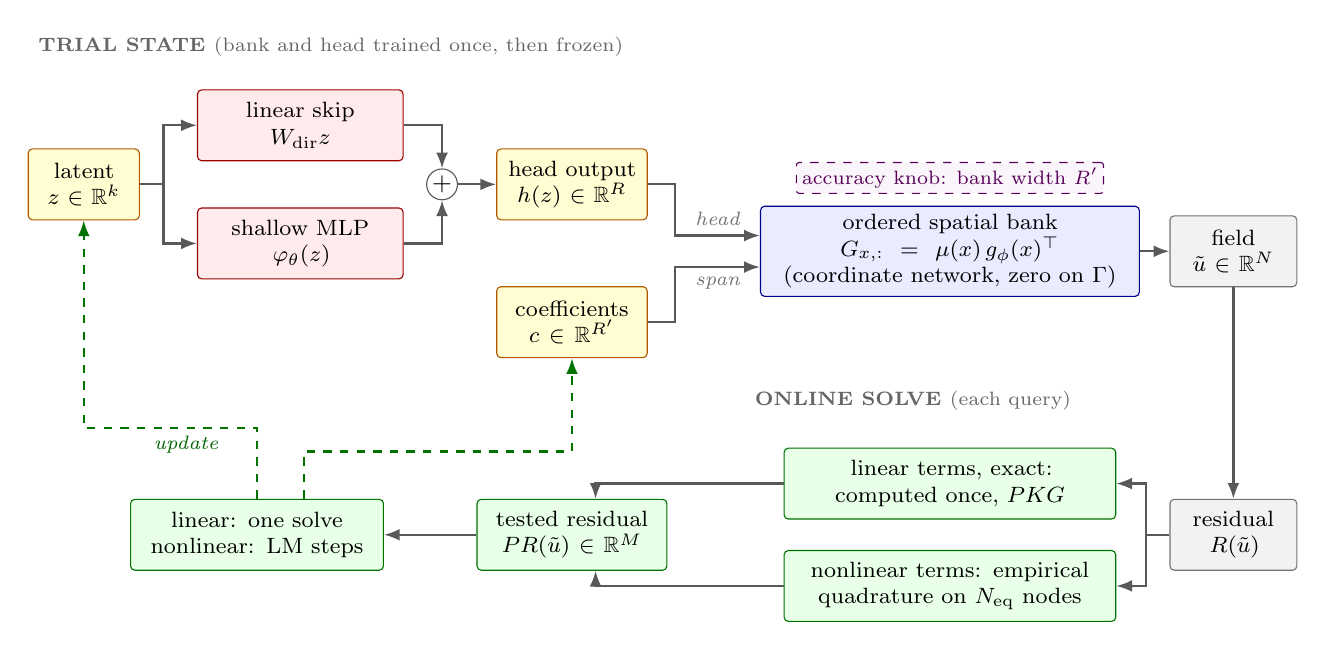
\begin{tikzpicture}[
  font=\footnotesize,
  box/.style={draw, rounded corners=1.5pt, minimum height=9mm, align=center,
              inner sep=3pt},
  dec/.style={box, fill=red!8, draw=red!60!black, text width=24mm},
  latent/.style={box, fill=yellow!18, draw=orange!70!black},
  bank/.style={box, fill=blue!8, draw=blue!55!black, text width=46mm},
  io/.style={box, fill=gray!10, draw=black!55},
  solve/.style={box, fill=green!9, draw=green!45!black},
  sum/.style={circle, draw=black!65, fill=white, inner sep=0.6pt, font=\small},
  knob/.style={draw=violet!70!black, dashed, rounded corners=1pt, fill=violet!4,
               font=\scriptsize, inner sep=2pt, text=violet!70!black},
  arr/.style={-{Latex[length=2mm]}, thick, draw=black!65},
  upd/.style={-{Latex[length=2mm]}, thick, dashed, draw=green!45!black},
  lbl/.style={font=\scriptsize\itshape, text=black!55},
  row/.style={font=\scriptsize\bfseries, text=black!60, anchor=west}
]
  % ===== TOP ROW: the trial state =====
  \node[row] at (-0.7,1.75) {TRIAL STATE \textmd{(bank and head trained once, then frozen)}};

  \node[latent, text width=12mm] (z) at (0,0) {latent\\$z\in\Real^{k}$};
  \node[dec] (skip) at (2.75,0.75) {linear skip\\$W_{\mathrm{dir}} z$};
  \node[dec] (mlp) at (2.75,-0.75) {shallow MLP\\$\varphi_\theta(z)$};
  \node[sum] (s1) at (4.55,0) {$+$};
  \node[latent, text width=17mm] (h) at (6.2,0) {head output\\$\head(z)\in\Real^{R}$};
  \node[latent, text width=17mm] (c) at (6.2,-1.75) {coefficients\\$c\in\Real^{R'}$};
  \node[bank] (G) at (11.0,-0.85) {ordered spatial bank\\$\bank_{x,:}=\bcmask(x)\,g_\phi(x)\T$\\(coordinate network, zero on $\Gamma$)};
  \node[io, text width=14mm] (u) at (14.6,-0.85) {field\\$\tilde u\in\Real^{N}$};

  \draw[arr] (z.east) -- ++(0.3,0) |- (skip.west);
  \draw[arr] (z.east) -- ++(0.3,0) |- (mlp.west);
  \draw[arr] (skip.east) -| (s1.north);
  \draw[arr] (mlp.east) -| (s1.south);
  \draw[arr] (s1) -- (h);
  \draw[arr] (h.east) -- ++(0.35,0) |- ([yshift=2mm]G.west)
       node[pos=0.75, above, lbl] {head};
  \draw[arr] (c.east) -- ++(0.35,0) |- ([yshift=-2mm]G.west)
       node[pos=0.75, below, lbl] {span};
  \draw[arr] (G) -- (u);

  \node[knob, above=1.5mm of G] {accuracy knob: bank width $R'$};

  % ===== BOTTOM ROW: online solve =====
  \node[row] at (8.4,-2.75) {ONLINE SOLVE \textmd{(each query)}};

  \node[io, text width=14mm] (res) at (14.6,-4.45) {residual\\$R(\tilde u)$};
  \node[solve, text width=40mm] (lin) at (11.0,-3.8) {linear terms, exact:\\computed once, $PKG$};
  \node[solve, text width=40mm] (eq) at (11.0,-5.1) {nonlinear terms: empirical\\quadrature on $N_{\mathrm{eq}}$ nodes};
  \node[solve, text width=22mm] (rw) at (6.2,-4.45) {tested residual\\$P R(\tilde u)\in\Real^{M}$};
  \node[solve, text width=30mm] (lm) at (2.2,-4.45) {linear: one solve\\nonlinear: LM steps};

  \draw[arr] (u) -- (res);
  \draw[arr] (res.west) -- ++(-0.3,0) |- (lin.east);
  \draw[arr] (res.west) -- ++(-0.3,0) |- (eq.east);
  \draw[arr] (lin.west) -| ([xshift=3mm]rw.north);
  \draw[arr] (eq.west) -| ([xshift=3mm]rw.south);
  \draw[arr] (rw) -- (lm);
  \draw[upd] (lm.north) -- ++(0,0.9) -| (z.south);
  \draw[upd] ([xshift=6mm]lm.north) -- ++(0,0.6) -| (c.south);
  \node[lbl, text=green!40!black] at (1.3,-3.3) {update};

\end{tikzpicture} {}}
\caption{NM-ROM model and online solve. \textbf{Top, trained once and
frozen:} the latent code $z$ passes through a linear skip and a shallow
SiLU network to give the bank coefficients $\head(z)$, and the ordered
coordinate-network bank, zero on $\Gamma$, turns them into the field
$\tilde u$. A query uses the head, $\tilde u=G h(z)$, or the span of the
first $R'$ ordered columns, $\tilde u=\widehat G_{R'}c$. \textbf{Bottom,
each query:} the residual is tested against $M$ fixed tests $P$, with
linear terms from the precomputed $PKG$ and advection from empirical
quadrature on $N_{\mathrm{eq}}$ nodes. A linear PDE in the span is one
least-squares solve; otherwise Levenberg--Marquardt steps update $z$ or
$c$. Dashed tags mark deployment choices.}
\label{fig:decoder}
\end{figure}

\paragraph{Where our method sits.}
Two families of methods make PDE solutions cheaper to compute, and they
differ in whether they solve the PDE online. \emph{Projection-based
reduced-order models} build a trial space offline from full-order
solutions and, for each query, solve the discretised PDE restricted to
that space. \emph{Neural operators} learn the map from inputs to
solutions and return a forward pass of the trained network, without
evaluating the PDE. Our method is a projection-based nonlinear-manifold
ROM, solved by least-squares Petrov--Galerkin projection; we compare
against both families.

\paragraph{Projection-based ROMs.}
Linear ROMs approximate solutions in a fixed subspace
\citep{BennerGugercinWillcox2015,Sirovich1987POD}; moving fronts can
require a large basis \citep{CohenDeVore2015,GreifUrban2019,Peherstorfer2022Kolmogorov}.
Nonlinear-manifold ROMs replace the subspace by a learned manifold and
keep the residual projection
\citep{LeeCarlberg2020,KimChoi2022NMROM,Romor2023NMROM,Diaz2024DDNMROM},
including quadratic manifolds \citep{GeelenWrightWillcox2022,BarnettFarhat2022},
neural-network corrections to a linear basis \citep{Barnett2023NNPROM},
adaptive bases \citep{PeherstorferWillcox2015Adaptive,Carlberg2015hRefinement},
hyper-reduced models of Navier--Stokes flows \citep{Romor2025Explicable}
and graph autoencoders on unstructured meshes \citep{Magargal2025GraphAE}.
These methods solve the PDE online, but a linear or quadratic basis is
tied to the mesh it was built on, and an autoencoder decoder is evaluated
at every node in each online iteration unless it is hyper-reduced.
Latent-dynamics ROMs instead learn the reduced dynamics from data
\citep{Fries2022LaSDI,He2023gLaSDI}.
Least-squares Petrov--Galerkin projection \citep{Carlberg2011LSPG} and
preassembly of reduced operators
\citep{StefanescuSandu2014,WederSchwerdtnerPeherstorfer2024} are
established components that we reuse. Our closest relatives are
neural-field ROMs \citep{Chen2023CROM,KimWenLeeChoiCNFROM2024,Berman2024CoLoRA}, which
also evaluate a coordinate network at individual nodes. We differ in
three ways: our decoder separates space from the latent code (a bank
times a head), so every linear term is precomputed exactly; the bank
carries an exact Dirichlet factor; and the bank is ordered after
training, so its nested widths give accuracy settings at query time
from one trained model, as runtime-tunable networks do for vision and
language models
\citep{YuSlimmable2019,Cai2020OnceForAll,Kusupati2022MRL,Devvrit2024MatFormer}.

\paragraph{Neural operators.}
FNO \citep{Li2020FNO}, DeepONet \citep{Lu2021DeepONet}, U-Net
\citep{Ronneberger2015UNet,Takamoto2022PDEBench} and Transolver
\citep{WuTransolver2024,Luo2025Transolverpp} learn solution maps, as do
neural-field operators \citep{Serrano2023CORAL} and pretrained PDE
foundation models \citep{Herde2024Poseidon,Hao2024DPOT}.
Their resolution or inference procedure can change accuracy and cost;
our accuracy setting instead changes the trial space in which the PDE
residual is solved.

\paragraph{Hyper-reduction and baselines.}
Empirical quadrature \citep{Hernandez2017EQ,YanoPatera2019LPEQ,Hernandez2024CECM}
reduces nonlinear residual evaluation through non-negative weights; we
retain that construction and test its error on the states the solver
reaches. Because learned solvers are often compared with weak baselines
\citep{McGreivy2024Weak}, we compare against named iterative full-order
solvers.

\section{Methodology}\label{sec:method}
\edef\restoredisplays{%
  \noexpand\abovedisplayskip=\the\abovedisplayskip
  \noexpand\belowdisplayskip=\the\belowdisplayskip
  \noexpand\abovedisplayshortskip=\the\abovedisplayshortskip
  \noexpand\belowdisplayshortskip=\the\belowdisplayshortskip}
\setlength{\abovedisplayskip}{1pt plus 1pt minus 1pt}
\setlength{\belowdisplayskip}{1pt plus 1pt minus 1pt}
\setlength{\abovedisplayshortskip}{1pt plus 1pt minus 1pt}
\setlength{\belowdisplayshortskip}{1pt plus 1pt minus 1pt}

A full-order solve has one unknown per grid node, so its cost grows with
the mesh size $N$. For each query we instead solve the same discretised
PDE in a few unknowns, at a cost that barely depends on $N$. This needs
three ingredients. First, a compact set of candidate solutions, the trial
manifold (\S\ref{sec:method:manifold}): the solution is a weighted sum of
the functions in the spatial bank, and its weights are either produced by
the nonlinear head from a few latent unknowns or solved for directly on
the first $R'$ bank functions. Second, a way to choose the right
candidate without knowing the answer (\S\ref{sec:method:weak}). Third, a
way to evaluate the PDE without visiting all $N$ nodes
(\S\ref{sec:method:precomp}): linear terms are computed once offline, and
the nonlinear term is sampled at a few nodes (in three dimensions, it is
evaluated with a precomputed quadratic tensor). Figure~\ref{fig:decoder} shows the whole pipeline. Throughout, $u\in\Real^{N}$ is the full-order discrete state
on a uniform grid and $K\in\Real^{N\times N}$ is the sparse
finite-difference matrix of $-\Delta$.



\subsection{Trial Manifold with Exact Dirichlet Enforcement}
\label{sec:method:manifold}

Solutions of one PDE family share their spatial structure, so a few
learned functions of space can describe all of them; the nonlinear head
lets their combination follow features, such as moving fronts, that a
small fixed combination misses. We do not use an encoder. The decoder writes the state as a fixed set of
spatial functions times coefficients produced by a small network,
\begin{equation}
  \tilde u(z) = \mathcal D(z) = G\,h(z),
  \qquad
  G_{x,:} = \mu(x)\,g_\phi(x)\T,
  \qquad
  \mu(x) = 16\,x_1(1-x_1)\,x_2(1-x_2).
  \label{eq:bank}
\end{equation}
Each column of the bank $G\in\Real^{N\times R}$ is one spatial function.
The function comes from a small network $g_\phi$ that takes the
coordinates of a point and returns a value there, so a column is simply
that network evaluated at every grid node. The head
$h:\Real^{k}\to\Real^{R}$ takes the latent state $z$ and returns one
weight per column. Because $\mu$ is zero on the boundary $\Gamma$, every
column of $G$ is zero there too. The boundary values therefore never
change when $z$ changes, on any mesh, and the boundary equations do not enter the solve. 
%The cube and the L-shaped domain use their own factor, which is zero on their boundaries in the same way. 
The cube and the L-shaped domain define their own boundary factor (Appendix~ \ref{app:method}), zero on their boundaries in the same way.
%For each new problem, we find $z$ by solving the PDE 
Each query then solves for $z$ (head) or $c$ (span) by solving the PDE
(\S\ref{sec:method:weak}).

\paragraph{Ordering the bank.}
\label{sec:method:ladder}\label{sec:method:ordered}
Training does not rank the columns of $G$: any one of them may matter as
much as any other, so keeping only the first $R'$ columns would throw
away useful ones at random. After training we therefore replace the
columns by new combinations of them, sorted from most to least important,
\begin{equation}
  \widehat G = G\,T .
  \label{eq:ordered}
\end{equation}
The matrix $T$ comes from a principal component analysis of the training
fields written in the bank (Appendix~\ref{app:method:ordered}). The first
column of $\widehat G$ is the single direction that best describes the
training fields, the second bests the remaining directions, and so on. Keeping
the first $R'$ columns therefore gives the best $R'$-dimensional subspace of the bank for the training data. At full width nothing changes: $\widehat G$
spans the same space as $G$, and no weight is retrained.
A query then solves in one of two ways,
\begin{equation}
  \tilde u = G\,h(z),\;\; z\in\Real^{k}
  \quad(\text{head}),
  \qquad
  \tilde u = \widehat G_{R'}\,c,\;\; c\in\Real^{R'}
  \quad(\text{span}),
  \label{eq:modes}
\end{equation}
where $\widehat G_{R'}$ holds the first $R'\le R$ columns. The head is a
nonlinear manifold with $k$ unknowns; the span is a linear space with $R'$
unknowns. The width $R'$ is the accuracy knob. The columns are nested, so
narrowing the span needs no retraining, and cheaper to solve and to convert back to a field.

\subsection{Projecting the PDE onto the Manifold}
\label{sec:method:weak}

At query time the solution is unknown but the PDE is known, so we choose
the candidate that best satisfies the discretised equations; no solution
data is needed at query time. Each PDE we consider gives a discretised residual $R(u)$ that vanishes at
the discrete solution. We substitute the trial manifold into $R$ and,
%instead of projecting with the decoder Jacobian, 
instead of pulling the residual back through the decoder Jacobian,
test it against $M$ fixed
vectors, the rows of $P\in\Real^{M\times N}$. On the square these are the
$M$ lowest sine modes, which are eigenvectors of $K$. 
%
% A query solves
A head query solves
\begin{equation}
  z^{\star} = \argmin_{z}\;\tfrac12\,\norm{P\,R\big(\tilde u(z)\big)}_2^2;
  \label{eq:objective}
\end{equation}
a span query solves the same problem in $c$.
We choose $M$ with the width: $M\ge k$ for the head and $M\ge R'$ for the span ($M=4R'$ for Burgers). 
%
This is least-squares Petrov--Galerkin projection \citep{Carlberg2011LSPG,LeeCarlberg2020} with fixed rather than state-dependent tests; each
row of $PR$ is also scaled by a fixed factor that puts the tests on a
common scale (Appendix~\ref{app:method}); we leave this scaling out of the
notation. We solve \eqref{eq:objective} by
damped Gauss--Newton (Levenberg--Marquardt) \citep{Marquardt1963},
\begin{equation}
  \Delta z = -\big(J\T J+\lambda\,\diag(J\T J)\big)^{-1}J\T P\,R\big(\tilde u(z)\big),
  \qquad
  J = P\,\frac{\partial R}{\partial u}\,J_{\mathcal D}(z),
  \label{eq:lm}
\end{equation}
and keep a step only if the residual decreases. Here
$J_{\mathcal D}(z)=G\,J_h(z)$ for the head and $J_{\mathcal D}=\widehat
G_{R'}$, a constant, for the span. Unlike $J_{\mathcal D}(z)\T$, the tests
$P$ do not change with $z$, which is what lets every linear term be
computed once (\S\ref{sec:method:precomp}). For Poisson in the span,
\eqref{eq:objective} is a linear least-squares problem solved once, and for
heat in the span each step is linear; the iteration is needed only for the
head and for the nonlinear PDEs.

\paragraph{Elliptic (Poisson).}
The Poisson residual is $R(u)=Ku-F$, where $F$ is the discrete source. In the span it is linear in $c$,
\begin{equation}
  P\,R\big(\widehat G_{R'}c\big) = \big(PK\widehat G_{R'}\big)\,c - PF,
  \label{eq:poisson-residual}
\end{equation}
so a query is one least-squares solve with a fixed $M\times R'$ matrix,
factorised once per mesh and width, and nothing is iterated. With the head,
\eqref{eq:lm} iterates in $z$ with $J=PKG\,J_h(z)$, and only the head is
re-evaluated.

\paragraph{Time-dependent problems.}
Heat (Crank--Nicolson), Burgers (backward Euler with a sign-upwind
stencil) and Navier--Stokes (implicit midpoint on the periodic cube) each
give a residual $R(u_{n+1})$ for one time step; their forms are in
Appendix~\ref{app:method}. Each step solves
\begin{equation}
  z_{n+1} = \argmin_{z}\;\norm{P\,R\big(\tilde u(z)\big)}_2,
  \qquad u_n=\tilde u(z_n),
  \label{eq:step}
\end{equation}
by \eqref{eq:lm}, warm-started from the previous step; the span solves the
same problem in $c_{n+1}$. The heat residual is linear, so in the span the
rollout applies one fixed $R'\times R'$ matrix per step. Burgers and
Navier--Stokes add a nonlinear advection term $A(u)$, so both the head and
the span iterate \eqref{eq:lm} at every step. For Navier--Stokes the tests
$P$ are divergence-free Fourier modes, so the pressure drops out of $PR$;
because the vortices travel, the bank is evaluated in a frame centred on
the flow whose shift is solved at each step (Appendix~\ref{app:method:ns}).

\subsection{Hyper-reduction}
\label{sec:method:precomp}

The manifold reduces the unknowns from $N$ to $k$ or $R'$, but the tested
residual $P\,R(\tilde u)$ still visits every node, so each evaluation costs
$O(NR)$, which would erase the wall-clock benefit. We remove this cost in two
ways, one for linear terms and one for the nonlinear term.

\paragraph{Linear terms: computed once and exact.}
A linear term is tested once, offline. For the Laplacian,
\begin{equation}
  P K\tilde u = \big(PKG\big)\,h(z),
  \qquad PKG\in\Real^{M\times R},
  \label{eq:preassembled}
\end{equation}
and the span uses $PK\widehat G_{R'}$, the first $R'$ columns of
$PKG\,T$. Online a linear term costs $O(MR)$ and is exact. For Poisson and
heat this is the whole residual, so their reduced solves make no
approximation beyond the trial space.

\paragraph{The nonlinear term: Empirical Quadrature.}
The advection terms of Burgers and Navier--Stokes cannot be computed once. We use Empirical Quadrature
\citep{Hernandez2017EQ,YanoPatera2019LPEQ} to select a non-negative
per-node weight vector $w$, independent of the state, such that
\begin{equation}
  P A(\tilde u) = \sum_{i=1}^{N} P_{:,i}\,A_i(\tilde u)
  \;\approx\; \sum_{i\in\mathcal S} w_i\,P_{:,i}\,A_i(\tilde u).
  \label{eq:eq-rule}
\end{equation}
Letting $g_i^{(\ell)}=P_{:,i}A_i(\tilde u^{(\ell)})\in\Real^{M}$ denote the
per-node contribution at a stored state $\tilde u^{(\ell)}$ that the solver
reaches on training trajectories, the constraint at that state is
$\sum_{i} w_i\,g_i^{(\ell)}=P A(\tilde u^{(\ell)})$. Stacking the
constraints gives a matrix $E$ and a vector $b$, and we solve
\begin{equation}
  \min_{w\ge 0}\;\norm{E\,w-b}_2
  \label{eq:nnls-main}
\end{equation}
by NNLS \citep{LawsonHanson1974NNLS}, which returns a sparse $w$ with
support $\mathcal S$ of size $N_{\mathrm{eq}}\ll N$. Computing $A_i$ needs
$\tilde u$ at node $i$ and its stencil neighbours $\mathcal N(i)$, so we
evaluate the decoder only on
$\mathcal S^{+}=\mathcal S\cup\bigcup_{i\in\mathcal S}\mathcal N(i)$, with
$|\mathcal S^{+}|\le 5N_{\mathrm{eq}}$ in two dimensions and $7N_{\mathrm{eq}}$ in three. Because each bank column is a
coordinate network (\S\ref{sec:decoder}), those rows of the bank are computed
once and cached.

\paragraph{Cost.}
With linear terms computed once and advection on $\mathcal S^{+}$, one
iteration of \eqref{eq:lm} costs
\begin{equation}
  \mathcal O\big(MR\,(N_{\mathrm{eq}}+k)\big),
  \label{eq:cost}
\end{equation}
with $k$ replaced by $R'$ in the span, plus the cost of the head and of
the small normal-equation solve, none of which depends on $N$. Returning the
field at an output time is one further $O(NR')$ product.

\paragraph{Checking the rule.}
Each rule is checked on the states the reduced solver reaches on
held-out trajectories, against an error bar fixed in advance; every rule
behind Table~\ref{tab:headline} passes (Appendix~\ref{app:method:eq}).

\subsection{Model Architecture}
\label{sec:decoder}

Three requirements of the solve shape the model in Figure~\ref{fig:decoder}. First, every head solve starts from a stored training code and descends along the head's Jacobian, so that Jacobian must retain a usable direction at all times; the linear skip guarantees this. Second, empirical quadrature keeps only a sparse set of nodes, which saves time only if the decoder can be evaluated at one node without the others --and one trained model must serve every mesh of a series; the coordinate-network bank meets both. Third, one trained model must offer several accuracy settings without retraining; the \emph{ordered bank} provides this.
Widths and training
settings are in Appendix~\ref{app:training-schedule}.

\paragraph{Linear skip, for the latent solve.}
The head is a shallow network plus a linear map,
\begin{equation}
  \head(\latent) \;=\; W_{\mathrm{dir}}\latent \;+\; \varphi_\theta(\latent),
  \qquad
  \varphi_\theta(\latent)=W_3\,\sigma\big(W_2\,\sigma(W_1\latent+b_1)+b_2\big)+b_3,
  \label{eq:head}
\end{equation}
with $\sigma$ the SiLU activation. Its Jacobian is
$\dhead(\latent)=W_{\mathrm{dir}}+J_{\varphi}(\latent)$. The first term does not
depend on $\latent$, so the Levenberg--Marquardt step from a stored code
always has a fixed linear direction to follow, while $\varphi_\theta$
supplies the curvature of the manifold. The head acts on the $R$ bank
coefficients, not on the $N$ nodes, so its cost and its parameter count do
not depend on the mesh.

\paragraph{Coordinate-network bank, for node-local evaluation.}
Each column of the bank is a coordinate network read at the node and
multiplied by the boundary factor of \eqref{eq:bank},
\begin{equation}
  \bank_{x,r}=\bcmask(x)\,g_{\phi,r}(x),
  \qquad
  g_\phi(x)=\mathrm{MLP}_\phi\big(\gamma(x)\big),
  \quad
  \gamma(x)=\big[\cos(2\pi\Omega x),\;\sin(2\pi\Omega x)\big],
  \label{eq:coordnet}
\end{equation}
where $\gamma$ is a random-Fourier-feature embedding with a fixed random
frequency matrix $\Omega$ \citep{Tancik2020FourierFeatures}. Because
$g_\phi$ reads a coordinate, a row of $\bank$ is computed from its node
alone. A quadrature rule therefore needs only the rows of $\mathcal S^{+}$,
and the same trained network is sampled on every mesh. Two natural
alternatives fail one of these tests. A convolutional or attention
decoder couples its output nodes, so one node costs a pass over the whole
grid, and a learned dense readout stores $NR$ parameters and must be
retrained for each mesh. The parameter count of $g_\phi$ does not depend on $N$.

\paragraph{Ordered bank, for deployment-time accuracy.}
\label{sec:method:tuning}\label{sec:method:layers}
The ordering \eqref{eq:ordered} makes the settings nested, so one model
built with $R$ columns contains every smaller one, and the two solve modes
of \eqref{eq:modes} are its two ends: the span is a linear ROM in a learned
bank, and the head is a nonlinear-manifold ROM in $k$ unknowns that can
follow states no small span contains.




\subsection{Implementation and Training}
\label{sec:impl}
This subsection describes how a query runs on the GPU and how the model
is trained. The matrix $PKG$ is built once per mesh, so a linear term
costs one small matrix--vector product online, and in the span the
Jacobian is the fixed matrix $PK\widehat G_{R'}$. With the head, the
remaining factor is the head Jacobian, supplied by forward-mode automatic
differentiation \citep{Bradbury2018JAX}: $J=PKG\,J_h(z)$ with
$J_h v=\mathrm{JVP}(h,z,v)$. Each accepted step solves the small damped
normal equation directly, and advection reads the cached stencil on the
quadrature nodes (Appendix~\ref{app:method:burgers}). The ordered bank is
stored in column blocks at the tested widths, so a query at width $R'$
reads exactly $R'$ columns. Training uses training data only: the
coordinate network $g_\phi$ is fitted to the training states through
\eqref{eq:bank} and frozen; the head is then fitted to the bank
coefficients of those states, with one stored code per training state (an
auto-decoder); last, the bank is ordered once by \eqref{eq:ordered}, with
one QR and one SVD. Widths, cohorts and offline costs are in
Appendix~\ref{app:training-schedule}.

% =====================================================================
\section{Experimental Setup and Benchmark Problems}
\label{sec:setup}
\restoredisplays

\paragraph{Problems and references.}
We test the method on PDEs of increasing difficulty: two linear problems,
Poisson and heat, and two nonlinear ones, viscous Burgers and
incompressible Navier--Stokes. In two dimensions we solve Poisson on the
square, with an L-shaped domain as a check with a re-entrant corner, heat
and Burgers; in three dimensions Poisson, heat and Burgers on the cube
and Navier--Stokes on the periodic cube. Meshes and cohorts are in
Table~\ref{tab:problems}, the sampled families in Table~\ref{tab:spec} and
the three-dimensional configurations in Table~\ref{tab:config3d}.

\paragraph{Accuracy.}
We report the worst relative $L^2$ error over the stated cases and
requested times, in percent. Poisson uses the steady reference norm and
heat the current reference norm; Burgers and Navier--Stokes use the
initial-field norm over evolved times. Same-grid error measures the
reduction error against the converged discrete solution. Settings for a test cohort are fixed before its
cases are opened; all other cohorts are development cohorts.

\paragraph{Timing and speedup.}
Every accuracy--runtime pair comes from the same solver invocation, in
double precision, with GPU burn-in, synchronised timing and medians of
retained repetitions (protocol in Appendix~\ref{app:cg-current}). GPU
query time covers initialisation, the solve or rollout and the requested
device outputs. Training and compilation are offline costs. Speedup is
$S=T_{\mathrm{FOM}}/T_{\mathrm{method}}$ with both times from the same
allocation. Solves that miss their stopping rule are reported as such and
do not enter a speedup.

\paragraph{Baselines.}
Poisson and the L-shape are compared with conjugate gradients (CG), heat
with Crank--Nicolson stepping whose linear solve is CG (CN--CG), Burgers
with Newton--BiCGStab, and Navier--Stokes with the Fourier pseudo-spectral
solver that generated its data (Crank--Nicolson diffusion,
Adams--Bashforth advection; CNAB2). Each runs at its fastest tested
setting at least as accurate as the accurate NM-ROM setting.

\section{Numerical Experiments and Results}\label{sec:results}
We ask three questions, on linear (Poisson, heat) and nonlinear (Burgers,
Navier--Stokes) problems: how the NM-ROM compares with full-order solvers
(\S\ref{sec:results:fom}, Table~\ref{tab:headline}), with neural operators
and other ROMs (\S\ref{sec:results:neuralops}, Table~\ref{tab:operators}),
and which setting to choose (\S\ref{sec:results:tunability}).



\subsection{Accuracy and Speed against Full-Order Solvers}\label{sec:results:fom}
\label{sec:results:operators}\label{sec:exp:panel}

\begin{table}[t]
\centering
\caption{NM-ROM against the named full-order solver (FOM) at every problem
and mesh. \textbf{Both NM-ROM columns of a row come from one frozen model}:
\emph{accurate} is the most accurate tested setting and \emph{fast} the
cheapest tested setting whose worst error is below 5\,\% (except $R'=64$,
5.6\,\%, on the L-shape, Poisson on an L-shaped domain); settings and FOM tolerances are in
Table~\ref{tab:headline-times}. Error is the worst relative $L^2$ error
over the cases (\%). Speedup is the FOM's median time divided by the
NM-ROM's in the same GPU allocation, \textbf{bold} where the NM-ROM is
faster; the FOM is a standard iterative solver (CG, CN--CG, Newton--BiCGStab or
CNAB2) run at the loosest tested setting that is at least as accurate as
the accurate setting; looser settings we tested were less accurate than
the NM-ROM, so the FOM error is often below ours. Every row is on held-out test cases that were not used
to choose the accurate setting.}
\label{tab:headline}
{%
% Side-by-side layout of the generated Table 1 (values unchanged).
\scriptsize\setlength{\tabcolsep}{2.6pt}
\resizebox{\linewidth}{!}{%
\begin{tabular}{@{}llrrrrr@{\hspace{9pt}}llrrrrr@{}}
\toprule
\multicolumn{7}{@{}c}{\emph{Two-dimensional}} & \multicolumn{7}{c@{}}{\emph{Three-dimensional}} \\
\cmidrule(r{6pt}){1-7}\cmidrule(l){8-14}
 & & \multicolumn{2}{c}{Accurate} & \multicolumn{2}{c}{Fast} & FOM & & & \multicolumn{2}{c}{Accurate} & \multicolumn{2}{c}{Fast} & FOM \\
\cmidrule(lr){3-4}\cmidrule(lr){5-6}\cmidrule(r{6pt}){7-7}\cmidrule(lr){10-11}\cmidrule(lr){12-13}\cmidrule(l){14-14}
Problem & Mesh & Err. & Speedup & Err. & Speedup & Err. & Problem & Mesh & Err. & Speedup & Err. & Speedup & Err. \\
\midrule
Poisson & $256^{2}$ & 0.84 & \textbf{18.2$\times$} & 4.07 & \textbf{27.0$\times$} & 0.77 & Poisson & $32^3$ & 0.23 & \textbf{4.42$\times$} & 2.01 & \textbf{5.25$\times$} & 0.16 \\
 & $1024^2$ & 0.83 & \textbf{31.1$\times$} & 4.06 & \textbf{82.0$\times$} & 0.33 &  & $64^3$ & 0.23 & \textbf{8.07$\times$} & 1.98 & \textbf{11.8$\times$} & 0.11 \\
 & $2048^2$ & 0.83 & \textbf{64.4$\times$} & 4.06 & \textbf{221$\times$} & 0.22 &  & $128^3$ & 0.23 & \textbf{13.6$\times$} & 1.97 & \textbf{28.5$\times$} & 0.075 \\
 & $4096^2$ & 0.83 & \textbf{108$\times$} & 4.06 & \textbf{372$\times$} & 0.58 &  & $256^3$ & 0.23 & \textbf{19.3$\times$} & 1.96 & \textbf{47.6$\times$} & 0.17 \\
\addlinespace[3pt]
L-shape & $256^2$ & 2.02 & \textbf{32.1$\times$} & 5.61 & \textbf{34.7$\times$} & 1.08 & Heat & $32^{3}$ & 0.080 & \textbf{10.9$\times$} & 1.11 & \textbf{15.2$\times$} & 0.078 \\
 & $512^2$ & 2.00 & \textbf{50.1$\times$} & 5.60 & \textbf{58.5$\times$} & 0.74 &  & $64^{3}$ & 0.082 & \textbf{8.50$\times$} & 4.78 & \textbf{18.0$\times$} & 0.081 \\
 & $1024^2$ & 1.99 & \textbf{41.6$\times$} & 5.60 & \textbf{49.4$\times$} & 1.77 &  & $128^{3}$ & 0.083 & \textbf{5.79$\times$} & 4.78 & \textbf{20.9$\times$} & 0.082 \\
 & $2048^2$ & 1.99 & \textbf{78.4$\times$} & 5.60 & \textbf{97.5$\times$} & 1.18 &  & $256^3$ & 0.083 & \textbf{7.60$\times$} & 4.78 & \textbf{28.0$\times$} & 0.082 \\
\addlinespace[3pt]
Heat & $1024^2$ & 0.13 & \textbf{105$\times$} & 1.08 & \textbf{200$\times$} & 0.045 & Burgers & $64^3$ & 1.01 & 0.21$\times$ & 3.37 & \textbf{2.08$\times$} & 0.92 \\
 & $2048^2$ & 0.13 & \textbf{216$\times$} & 1.08 & \textbf{512$\times$} & 0.045 &  & $128^3$ & 1.46 & 0.57$\times$ & 4.26 & \textbf{5.10$\times$} & 1.39 \\
 & $4096^{2}$ & 0.13 & \textbf{231$\times$} & 1.08 & \textbf{491$\times$} & 0.054 &  & $256^3$ & 2.20 & \textbf{2.19$\times$} & 3.77 & \textbf{5.60$\times$} & 1.52 \\
\addlinespace[3pt]
Burgers & $256^2$ & 0.87 & 0.38$\times$ & 3.85 & \textbf{1.22$\times$} & 0.11 & Navier--Stokes & $32^3$ & 0.21 & 0.93$\times$ & 3.06 & \textbf{3.56$\times$} & 0.19 \\
 & $512^2$ & 1.13 & 0.62$\times$ & 4.10 & \textbf{1.93$\times$} & 0.12 &  & $64^3$ & 0.21 & \textbf{2.92$\times$} & 3.06 & \textbf{8.53$\times$} & 0.12 \\
 & $1024^2$ & 1.25 & \textbf{1.51$\times$} & 4.25 & \textbf{3.87$\times$} & 0.13 &  & $96^3$ & 0.21 & \textbf{8.01$\times$} & 3.24 & \textbf{14.4$\times$} & 0.056 \\
 & $2048^2$ & 1.32 & \textbf{3.39$\times$} & 3.06 & \textbf{8.72$\times$} & 0.13 &  &  &  &  &  &  &  \\
 & $4096^2$ & 1.35 & \textbf{10.7$\times$} & 3.11 & \textbf{27.5$\times$} & 0.14 &  &  &  &  &  &  &  \\
\bottomrule
\end{tabular}}}
\end{table}

Each row of Table~\ref{tab:headline} shows two settings of one trained
model, an accurate one and a fast one. The fast setting beats the
full-order solver on every problem and mesh; the accurate one beats it on
every linear problem and on the finer meshes of the nonlinear ones.

\paragraph{Linear problems.}
On Poisson, the L-shape and heat both settings of a row are solves in the
span of the ordered bank. The head is less accurate there
(4.48\,\% against 0.83\,\% on Poisson at $4096^2$, Table~\ref{tab:tunability}): on a linear problem the best solve in the bank is the linear
one, and it is also the cheapest. Because the reduced query does not visit
the grid until it returns the field, the speedup grows with the mesh, to
108$\times$ over CG on Poisson at $4096^2$ and
$\nHeatWideBatchedAccS\times$ over CN--CG on heat at $2048^2$.
The accurate error is the same at every mesh because it is the bank's
projection floor, the best fit of the same-grid solution in the span of
the frozen bank; the reduced solve reaches that floor (0.83\,\% on
Poisson), and the floor does not change once the solution is resolved.

\paragraph{Burgers.}
At coarse meshes the reduced solve is slower than Newton--BiCGStab, but its
cost barely changes with the mesh. On the 64 held-out test cases the
accurate setting (the span of 384) reaches 0.87--1.35\,\% (median
0.03\,\%) at 0.38--10.7$\times$ the speed of Newton--BiCGStab, and the fast
setting (the span of 96 up to $1024^2$ and of 128 beyond) 3.06--4.25\,\% at
1.22--27.5$\times$; the fast setting is faster than the FOM at every mesh and
the accurate one from $1024^2$.

In three dimensions one frozen span model, trained on $32^3$--$128^3$
fields and used unchanged at $256^3$, reaches 2.20\,\% at 2.19$\times$
the speed of Newton--BiCGStab at $256^3$, with settings chosen on 64
validation cases; advection uses a precomputed quadratic tensor, and the
nonlinear head did not generalise on this family and is not used.

\paragraph{Navier--Stokes.}
Here the head earns its place. On the held-out test cases the head with $k=\nNsHeadK$
reaches 0.21\,\% at every mesh, at 0.93$\times$, 2.92$\times$ and
8.01$\times$ the speed of CNAB2 at $32^3$, $64^3$ and $96^3$. The span of the same bank is
33$\times$ less accurate at the same number of unknowns, and
even the full rank-$\nNsBankR$ span reaches only 1.12\,\%:
the moving vortices lie on a curved manifold that no small span contains. The error stays flat from
$32^3$ to $96^3$ while the speedup rises.

\paragraph{Where the speedup comes from.}
On the linear problems the query does not iterate: it is one
least-squares solve with a matrix factorised offline, and its time is
mostly writing the $O(NR')$ output field (41.8 of 42.4\,ms on the Poisson
development cases at $4096^2$, where CG needs about 5300 iterations over all nodes). On the
nonlinear problems the iteration count does not grow with the mesh: about
one Levenberg--Marquardt iteration per time step on Burgers and three
Gauss--Newton sweeps on Navier--Stokes, each costing \eqref{eq:cost}
(Table~\ref{tab:iterations}). The full-order solvers sweep all $N$ nodes
in every iteration and, for CG, need more iterations as the mesh is
refined \citep{Saad2003}. At the settings of Table~\ref{tab:headline},
time grows as $N^{p}$ with $p\approx0.2$ for our model on Burgers and $0.3$
on Navier--Stokes, against about $0.8$ and $0.9$ for the full-order solvers.

\subsection{Comparison with Neural Operators and Other ROMs}\label{sec:results:neuralops}

We next compare with the two alternatives a practitioner would consider
instead: neural operators and other reduced-order models. We train an FNO \citep{Li2020FNO}, a U-Net \citep{Ronneberger2015UNet}, a
DeepONet \citep{Lu2021DeepONet} and a Transolver \citep{WuTransolver2024}, widely used representatives of spectral, convolutional,
branch--trunk and attention-based operators,
on the evaluation mesh, on our model's training split (on Burgers, 128 trajectories of the
same family) with a 3000\,s wall budget per network, and time them with the NM-ROM and the full-order solver in one
allocation per problem (Table~\ref{tab:operators}).

\begin{table}[t]
\centering
\caption{Best NM-ROM against FNO, U-Net, Transolver and DeepONet at every
measured (PDE, $N$) cell. Both NM-ROM columns come from the same trained
model. Error and speedup as in Table~\ref{tab:headline}, one full-order
setting per cell; \emph{italic} marks speedups below $1\times$. \textbf{Bold} marks an NM-ROM setting that is both more accurate
and faster than every operator in the cell. Each operator family shows the size chosen on its
validation cases; most operator runs stopped at the 3000\,s wall
budget (Table~\ref{tab:development-training}). Timed separately from
Table~\ref{tab:headline} (Appendix~\ref{app:operators}).}
\label{tab:operators}
\resizebox{\linewidth}{!}{%
\scriptsize\setlength{\tabcolsep}{3pt}
\begin{tabular}{@{}llrrrrrrrrrrrr@{}}
\toprule
 & & \multicolumn{2}{c}{NM-ROM accurate} & \multicolumn{2}{c}{NM-ROM second setting} & \multicolumn{2}{c}{FNO} & \multicolumn{2}{c}{U-Net} & \multicolumn{2}{c}{Transolver} & \multicolumn{2}{c}{DeepONet} \\
\cmidrule(lr){3-4}\cmidrule(lr){5-6}\cmidrule(lr){7-8}\cmidrule(lr){9-10}\cmidrule(lr){11-12}\cmidrule(l){13-14}
PDE & $N$ & Err.\ (\%) & Speedup & Err.\ (\%) & Speedup & Err.\ (\%) & Speedup & Err.\ (\%) & Speedup & Err.\ (\%) & Speedup & Err.\ (\%) & Speedup \\
\midrule
\multirow{3}{*}{Burgers 2D} & $256^2$ & --- & --- & 4.10 & \emph{0.58$\times$} & 8.76 & 2.53$\times$ & 5.98 & 1.83$\times$ & 6.83 & 1.64$\times$ & 64.2 & 4.79$\times$ \\
 & $1024^2$ & 1.25 & \emph{0.24$\times$} & \textbf{8.42} & \textbf{2.15$\times$} & 14.8 & \emph{0.74$\times$} & 11.5 & 1.38$\times$ & 14.9 & \emph{0.55$\times$} & 68.2 & 1.44$\times$ \\
 & $2048^2$ & 1.32 & 1.05$\times$ & \textbf{9.04} & \textbf{7.37$\times$} & 18.0 & \emph{0.31$\times$} & 22.6 & 1.42$\times$ & 33.8 & 1.43$\times$ & 67.1 & 1.96$\times$ \\
\midrule
\multirow{2}{*}{Heat 2D} & $1024^2$ & \textbf{0.13} & \textbf{87.4$\times$} & --- & --- & 3.59 & 1.07$\times$ & 1.56 & 1.93$\times$ & 2.57 & 6.22$\times$ & 4.60 & 2.09$\times$ \\
 & $2048^2$ & \textbf{0.13} & \textbf{289$\times$} & --- & --- & 3.98 & \emph{0.93$\times$} & 2.76 & 2.76$\times$ & 3.66 & 40.5$\times$ & 10.9 & 5.11$\times$ \\
\midrule
\multirow{3}{*}{Navier--Stokes 3D} & $32^3$ & 0.21 & \emph{0.94$\times$} & 3.24 & 1.68$\times$ & 0.53 & 1.69$\times$ & 0.68 & \emph{0.37$\times$} & 0.78 & \emph{0.34$\times$} & 51.9 & 1.52$\times$ \\
 & $64^3$ & \textbf{0.21} & \textbf{3.00$\times$} & 3.24 & 5.29$\times$ & 1.76 & 2.07$\times$ & 1.58 & \emph{0.75$\times$} & 1.80 & \emph{0.71$\times$} & 47.6 & 1.39$\times$ \\
 & $96^3$ & \textbf{0.21} & \textbf{8.01$\times$} & 3.24 & 14.4$\times$ & 1.51 & 3.23$\times$ & 2.29 & 1.44$\times$ & 1.16 & 6.65$\times$ & 51.4 & 2.26$\times$ \\
\bottomrule
\end{tabular}}
\end{table}

\paragraph{Against neural operators, the NM-ROM wins as the mesh grows.}
On small meshes the operators are competitive, since a forward pass is
cheap: at $256^2$ on Burgers all four are faster than the NM-ROM, and at
$32^3$ on Navier--Stokes the FNO is faster than our accurate setting and
more accurate than our fast one. As the mesh grows, the NM-ROM's
advantage grows with it: its query does not visit the grid until it
returns the field, while every operator reads and writes the full grid,
and the FNO, U-Net and Transolver errors on Burgers grow 2--5$\times$
from $256^2$ to $2048^2$. From $1024^2$ on, and on Navier--Stokes from
$64^3$, one NM-ROM setting is both more accurate and faster than all four
operators (Table~\ref{tab:operators}, bold): on Burgers 8.42--9.04\,\%
against 11.5--68.2\,\% for the operators, on heat 0.13\,\% against
1.56--10.9\,\%, and on Navier--Stokes 0.21\,\% against 1.16--51.4\,\%.

\paragraph{At the same number of unknowns, the learned manifold is far more accurate than prior ROMs.}
With 16 unknowns, a linear basis and a quadratic manifold cannot follow
the moving fronts of Burgers, and both run slower than the full-order
solver; our head follows them at a cost that does not grow with the
mesh. On the 64 test cases at $1024^2$ and $2048^2$, the head with
$k=16$ reaches 8.42--9.04\,\% at 2.17--4.79$\times$ the speed of
Newton--BiCGStab, against 34.1--41.7\,\% for POD-LSPG and a quadratic
manifold \citep{GeelenWrightWillcox2022} (Table~\ref{tab:nmrom-baselines}).
POD-LSPG approaches 1\,\% only with 256 or more unknowns, two orders of
magnitude slower, and its basis is rebuilt from 128 new full-order
trajectories at each mesh. A reproduced shallow masked-autoencoder
NM-ROM \citep{KimChoi2022NMROM} did not reach a usable accuracy in our
setting (145--175\,\%; Table~\ref{tab:nmrom-baselines}).



\subsection{Which Knob to Turn}\label{sec:results:tunability}\label{sec:results:best}

A user of the trained model can turn two knobs without retraining: the
bank width $R'$ and the choice between head and span (full ladders in
Table~\ref{tab:tunability}). The width changes what the model can
represent, so it is the accuracy knob. On Poisson at $4096^2$, narrowing the bank from
$R'=512$ to $32$ raises the error 18.6$\times$ and moves the
same model from 108$\times$ to 1136$\times$ the speed
of CG on the test cases. On heat at $2048^2$ the span runs from 0.13\,\% at 216$\times$
($R'=128$) to 1.08\,\% at 512$\times$ ($R'=32$), and on Burgers at
$4096^2$ from 1.35\,\% at 10.7$\times$ ($R'=384$) to 8.24\,\% at
44.5$\times$ ($R'=64$). The choice between head and span
depends on the problem: on the linear problems the span is both more
accurate and cheaper (\S\ref{sec:results:operators}), while on
Navier--Stokes the head is the accurate end, 33$\times$ more
accurate than the span at the same number of unknowns for about twice the
cost.

\paragraph{Limitations.}\label{sec:limitations}
\label{sec:results:head}\label{sec:results:collapse}\label{sec:exp:eq}
(i) Except for Navier--Stokes, speedups are against named iterative
full-order solvers at the stated tolerances. Fast direct and spectral
solvers exist for the square and the cube and would be faster than CG
there.
(ii) The Navier--Stokes bank is a POD basis built at each mesh and
evaluated in a moving frame, with a head trained at each mesh, and the
family has moderate Reynolds numbers; we make
no claim about turbulent flow.
(iii) On the L-shape the available tests limit the span to width 128.
(iv) Quadrature validation covers finitely many reached states and is not
a global certificate, and we changed the check once after seeing results
(\S\ref{sec:method:precomp}). Reduced
solves can converge to a wrong branch, and lower same-grid error does not
remove discretisation error.
(v) The evaluation cohorts are small (6--64 cases). Timings report medians without dispersion.

\section{Conclusion and Future Work}\label{sec:conclusion}

We built an NM-ROM whose speedup grows with the mesh: it is up
to 27.5$\times$ faster than the full-order solver on nonlinear problems and
over 100$\times$ faster on linear ones. One trained model also offers
several accuracy settings at query time, through the width of its ordered
bank and the choice between head and span, whereas a trained neural
operator gives one fixed point at a given mesh. Next are higher-Reynolds-number
flows and a nonlinear head for three-dimensional Burgers.

\section*{Ethics statement}
This work develops numerical methods for solving partial differential
equations. All data are synthetic, generated by numerical solvers from
sampled parameters; no human subjects, personal data or released datasets
are involved. We are not aware of harmful uses beyond those of
general-purpose simulation software.

\section*{Reproducibility statement}\label{sec:repro}
Every table and prose number is taken from versioned run records
identifying source, checkpoint, settings, cohort, allocation and audit
(Appendix~\ref{app:provenance}); failed settings are kept.

\section*{AI use statement}
AI coding agents (Claude, Codex) implemented the methods,
baselines and pipelines, proposed and refined experiment designs,
analysed and cross-checked results, and drafted and edited text. Every
reported number comes from a recorded solver run
(Appendix~\ref{app:provenance}). The authors reviewed this work and take
responsibility for all content.

\enlargethispage{\baselineskip}
\bibliographystyle{plainnat}
%
\begin{thebibliography}{99}

\bibitem[Azizzadenesheli et~al.(2024)]{Azizzadenesheli2024NatRevPhys}
K.~Azizzadenesheli, N.~Kovachki, Z.~Li, M.~Liu-Schiaffini, J.~Kossaifi, and
A.~Anandkumar.
\newblock Neural operators for accelerating scientific simulations and design.
\newblock \emph{Nature Reviews Physics}, 6(5):320--328, 2024.

\bibitem[Barnett and Farhat(2022)]{BarnettFarhat2022}
J.~Barnett and C.~Farhat.
\newblock Quadratic approximation manifold for mitigating the
Kolmogorov barrier in nonlinear projection-based model order reduction.
\newblock \emph{Journal of Computational Physics}, 464:111348, 2022.

\bibitem[Barnett et~al.(2023)]{Barnett2023NNPROM}
J.~Barnett, C.~Farhat, and Y.~Maday.
\newblock Neural-network-augmented projection-based model order reduction for
mitigating the {K}olmogorov barrier to reducibility.
\newblock \emph{Journal of Computational Physics}, 492:112420, 2023.

\bibitem[Benner et~al.(2015)]{BennerGugercinWillcox2015}
P.~Benner, S.~Gugercin, and K.~Willcox.
\newblock A survey of projection-based model reduction methods for
parametric dynamical systems.
\newblock \emph{SIAM Review}, 57(4):483--531, 2015.

\bibitem[Berman and Peherstorfer(2024)]{Berman2024CoLoRA}
J.~Berman and B.~Peherstorfer.
\newblock {CoLoRA}: Continuous low-rank adaptation for reduced implicit neural
modeling of parameterized partial differential equations.
\newblock In \emph{Proceedings of the 41st International Conference on Machine
Learning}, volume 235 of \emph{PMLR}, pages 3565--3583, 2024.

\bibitem[Bradbury et~al.(2018)]{Bradbury2018JAX}
J.~Bradbury, R.~Frostig, P.~Hawkins, M.~J. Johnson, C.~Leary,
D.~Maclaurin, G.~Necula, A.~Paszke, J.~VanderPlas, S.~Wanderman-Milne,
and Q.~Zhang.
\newblock JAX: composable transformations of Python+NumPy programs, 2018.

\bibitem[Cai et~al.(2020)]{Cai2020OnceForAll}
H.~Cai, C.~Gan, T.~Wang, Z.~Zhang, and S.~Han.
\newblock Once-for-All: Train one network and specialize it for
efficient deployment.
\newblock In \emph{International Conference on Learning Representations},
2020.

\bibitem[Carlberg(2015)]{Carlberg2015hRefinement}
K.~Carlberg.
\newblock Adaptive $h$-refinement for reduced-order models.
\newblock \emph{International Journal for Numerical Methods in Engineering},
102(5):1192--1210, 2015.

\bibitem[Carlberg et~al.(2011)]{Carlberg2011LSPG}
K.~Carlberg, C.~Bou-Mosleh, and C.~Farhat.
\newblock Efficient non-linear model reduction via a least-squares
Petrov--Galerkin projection and compressive tensor approximations.
\newblock \emph{International Journal for Numerical Methods in
Engineering}, 86(2):155--181, 2011.

\bibitem[Chen et~al.(2023)]{Chen2023CROM}
P.~Y. Chen, J.~Xiang, D.~H. Cho, Y.~Chang, G.~A. Pershing, H.~T. Maia,
M.~M. Chiaramonte, K.~T. Carlberg, and E.~Grinspun.
\newblock {CROM}: Continuous reduced-order modeling of {PDE}s using implicit
neural representations.
\newblock In \emph{International Conference on Learning Representations},
2023.

\bibitem[Cohen and DeVore(2015)]{CohenDeVore2015}
A.~Cohen and R.~DeVore.
\newblock Approximation of high-dimensional parametric PDEs.
\newblock \emph{Acta Numerica}, 24:1--159, 2015.

\bibitem[Devvrit et~al.(2024)]{Devvrit2024MatFormer}
Devvrit, S.~Kudugunta, A.~Kusupati, T.~Dettmers, K.~Chen, I.~Dhillon,
Y.~Tsvetkov, H.~Hajishirzi, S.~Kakade, A.~Farhadi, and P.~Jain.
\newblock {MatFormer}: Nested transformer for elastic inference.
\newblock In \emph{Advances in Neural Information Processing Systems},
volume~37, pages 140535--140564, 2024.

\bibitem[Diaz et~al.(2024)]{Diaz2024DDNMROM}
A.~N. Diaz, Y.~Choi, and M.~Heinkenschloss.
\newblock A fast and accurate domain decomposition nonlinear manifold reduced
order model.
\newblock \emph{Computer Methods in Applied Mechanics and Engineering},
425:116943, 2024.

\bibitem[Fries et~al.(2022)]{Fries2022LaSDI}
W.~D. Fries, X.~He, and Y.~Choi.
\newblock {LaSDI}: Parametric latent space dynamics identification.
\newblock \emph{Computer Methods in Applied Mechanics and Engineering},
399:115436, 2022.

\bibitem[Geelen et~al.(2022)]{GeelenWrightWillcox2022}
R.~Geelen, S.~Wright, and K.~Willcox.
\newblock Operator inference for non-intrusive model reduction with
quadratic manifolds.
\newblock \emph{Computer Methods in Applied Mechanics and Engineering},
403:115717, 2022.

\bibitem[Golub and Pereyra(1973)]{GolubPereyra1973}
G.~H. Golub and V.~Pereyra.
\newblock The differentiation of pseudo-inverses and nonlinear least squares
problems whose variables separate.
\newblock \emph{SIAM Journal on Numerical Analysis}, 10(2):413--432, 1973.

\bibitem[Greif and Urban(2019)]{GreifUrban2019}
C.~Greif and K.~Urban.
\newblock Decay of the Kolmogorov $N$-width for wave problems.
\newblock \emph{Applied Mathematics Letters}, 96:216--222, 2019.

\bibitem[Hao et~al.(2024)]{Hao2024DPOT}
Z.~Hao, C.~Su, S.~Liu, J.~Berner, C.~Ying, H.~Su, A.~Anandkumar, J.~Song,
and J.~Zhu.
\newblock {DPOT}: Auto-regressive denoising operator transformer for
large-scale {PDE} pre-training.
\newblock In \emph{International Conference on Machine Learning}, pages
17616--17635, 2024.

\bibitem[He et~al.(2023)]{He2023gLaSDI}
X.~He, Y.~Choi, W.~D. Fries, J.~L. Belof, and J.-S. Chen.
\newblock {gLaSDI}: Parametric physics-informed greedy latent space dynamics
identification.
\newblock \emph{Journal of Computational Physics}, 489:112267, 2023.

\bibitem[Herde et~al.(2024)]{Herde2024Poseidon}
M.~Herde, B.~Raoni{\'c}, T.~Rohner, R.~K{\"a}ppeli, R.~Molinaro,
E.~de~B{\'e}zenac, and S.~Mishra.
\newblock Poseidon: Efficient foundation models for {PDE}s.
\newblock In \emph{Advances in Neural Information Processing Systems},
volume~37, pages 72525--72624, 2024.

\bibitem[Hern\'andez et~al.(2017)]{Hernandez2017EQ}
J.~A. Hern\'andez, M.~A. Caicedo, and A.~Ferrer.
\newblock Dimensional hyper-reduction of nonlinear finite element
models via empirical cubature.
\newblock \emph{Computer Methods in Applied Mechanics and Engineering},
313:687--722, 2017.

\bibitem[Hern\'andez et~al.(2024)]{Hernandez2024CECM}
J.~A. Hern\'andez, J.~R. Bravo, and S.~Ares~de~Parga.
\newblock {CECM}: A continuous empirical cubature method with application to
the dimensional hyperreduction of parameterized finite element models.
\newblock \emph{Computer Methods in Applied Mechanics and Engineering},
418:116552, 2024.

\bibitem[Hestenes and Stiefel(1952)]{HestenesStiefel1952CG}
M.~R. Hestenes and E.~Stiefel.
\newblock Methods of conjugate gradients for solving linear systems.
\newblock \emph{Journal of Research of the National Bureau of Standards},
49(6):409--436, 1952.

\bibitem[Hesthaven et~al.(2026)]{Hesthaven2026Transport}
J.~S. Hesthaven, B.~Peherstorfer, and B.~Unger.
\newblock Nonlinear model reduction for transport-dominated problems.
\newblock \emph{arXiv preprint arXiv:2602.01397}, 2026.

\bibitem[Holzschuh et~al.(2025)]{Holzschuh2025PDETransformer}
B.~Holzschuh, Q.~Liu, G.~Kohl, and N.~Thuerey.
\newblock {PDE-Transformer}: Efficient and versatile transformers for physics
simulations.
\newblock In \emph{Proceedings of the 42nd International Conference on Machine
Learning}, 2025.

\bibitem[de~Hoop et~al.(2022)]{deHoop2022CostAccuracy}
M.~V. de~Hoop, D.~Z. Huang, E.~Qian, and A.~M. Stuart.
\newblock The cost-accuracy trade-off in operator learning with neural networks.
\newblock \emph{Journal of Machine Learning}, 1(3):299--341, 2022.

\bibitem[Y.~Kim et~al.(2022)]{KimChoi2022NMROM}
Y.~Kim, Y.~Choi, D.~Widemann, and T.~Zohdi.
\newblock A fast and accurate physics-informed neural network reduced
order model with shallow masked autoencoder.
\newblock \emph{Journal of Computational Physics}, 451:110841, 2022.

\bibitem[M.~Kim et~al.(2024)]{KimWenLeeChoiCNFROM2024}
M.~Kim, T.~Wen, K.~Lee, and Y.~Choi.
\newblock Physics-informed reduced order model with conditional neural
fields.
\newblock \emph{arXiv preprint arXiv:2412.05233}, 2024.

\bibitem[Kovachki et~al.(2023)]{Kovachki2023NeuralOperator}
N.~Kovachki, Z.~Li, B.~Liu, K.~Azizzadenesheli, K.~Bhattacharya,
A.~Stuart, and A.~Anandkumar.
\newblock Neural operator: learning maps between function spaces.
\newblock \emph{Journal of Machine Learning Research}, 24(89):1--97,
2023.

\bibitem[Kusupati et~al.(2022)]{Kusupati2022MRL}
A.~Kusupati, G.~Bhatt, A.~Rege, M.~Wallingford, A.~Sinha, V.~Ramanujan,
W.~Howard-Snyder, K.~Chen, S.~Kakade, P.~Jain, and A.~Farhadi.
\newblock Matryoshka representation learning.
\newblock In \emph{Advances in Neural Information Processing Systems},
volume~35, pages 30233--30249, 2022.

\bibitem[Lawson and Hanson(1974)]{LawsonHanson1974NNLS}
C.~L. Lawson and R.~J. Hanson.
\newblock \emph{Solving Least Squares Problems}.
\newblock Prentice-Hall, Englewood Cliffs, NJ, 1974.

\bibitem[Lee and Carlberg(2020)]{LeeCarlberg2020}
K.~Lee and K.~T. Carlberg.
\newblock Model reduction of dynamical systems on nonlinear manifolds
using deep convolutional autoencoders.
\newblock \emph{Journal of Computational Physics}, 404:108973, 2020.

\bibitem[Li et~al.(2021)]{Li2020FNO}
Z.~Li, N.~Kovachki, K.~Azizzadenesheli, B.~Liu, K.~Bhattacharya,
A.~Stuart, and A.~Anandkumar.
\newblock Fourier neural operator for parametric partial differential
equations.
\newblock In \emph{International Conference on Learning Representations},
2021.

\bibitem[Lu et~al.(2021)]{Lu2021DeepONet}
L.~Lu, P.~Jin, G.~Pang, Z.~Zhang, and G.~E. Karniadakis.
\newblock Learning nonlinear operators via DeepONet based on the
universal approximation theorem of operators.
\newblock \emph{Nature Machine Intelligence}, 3(3):218--229, 2021.

\bibitem[Luo et~al.(2025)]{Luo2025Transolverpp}
H.~Luo, H.~Wu, H.~Zhou, L.~Xing, Y.~Di, J.~Wang, and M.~Long.
\newblock Transolver++: An accurate neural solver for {PDE}s on million-scale
geometries.
\newblock In \emph{International Conference on Machine Learning}, pages
41432--41449, 2025.

\bibitem[Magargal et~al.(2025)]{Magargal2025GraphAE}
L.~Magargal, P.~Khodabakhshi, S.~Rodriguez, J.~Jaworski, and J.~Michopoulos.
\newblock Projection-based model-order reduction via graph autoencoders suited
for unstructured meshes.
\newblock \emph{Data-Centric Engineering}, 6:e52, 2025.

\bibitem[Marquardt(1963)]{Marquardt1963}
D.~W. Marquardt.
\newblock An algorithm for least-squares estimation of nonlinear parameters.
\newblock \emph{Journal of the Society for Industrial and Applied Mathematics},
11(2):431--441, 1963.

\bibitem[McGreivy and Hakim(2024)]{McGreivy2024Weak}
N.~McGreivy and A.~Hakim.
\newblock Weak baselines and reporting biases lead to overoptimism in machine
learning for fluid-related partial differential equations.
\newblock \emph{Nature Machine Intelligence}, 6(10):1256--1269, 2024.

\bibitem[Peherstorfer(2022)]{Peherstorfer2022Kolmogorov}
B.~Peherstorfer.
\newblock Breaking the {K}olmogorov barrier with nonlinear model reduction.
\newblock \emph{Notices of the American Mathematical Society}, 69(5):725--733,
2022.

\bibitem[Peherstorfer and Willcox(2015)]{PeherstorferWillcox2015Adaptive}
B.~Peherstorfer and K.~Willcox.
\newblock Online adaptive model reduction for nonlinear systems via low-rank
updates.
\newblock \emph{SIAM Journal on Scientific Computing}, 37(4):A2123--A2150, 2015.

\bibitem[Romor et~al.(2023)]{Romor2023NMROM}
F.~Romor, G.~Stabile, and G.~Rozza.
\newblock Non-linear manifold reduced-order models with convolutional
autoencoders and reduced over-collocation method.
\newblock \emph{Journal of Scientific Computing}, 94(3):74, 2023.

\bibitem[Romor et~al.(2025)]{Romor2025Explicable}
F.~Romor, G.~Stabile, and G.~Rozza.
\newblock Explicable hyper-reduced order models on nonlinearly approximated
solution manifolds of compressible and incompressible {N}avier--{S}tokes
equations.
\newblock \emph{Journal of Computational Physics}, 524:113729, 2025.

\bibitem[Ronneberger et~al.(2015)]{Ronneberger2015UNet}
O.~Ronneberger, P.~Fischer, and T.~Brox.
\newblock {U-Net}: Convolutional networks for biomedical image segmentation.
\newblock In \emph{Medical Image Computing and Computer-Assisted Intervention
(MICCAI)}, pages 234--241, 2015.

\bibitem[Saad(2003)]{Saad2003}
Y.~Saad.
\newblock \emph{Iterative Methods for Sparse Linear Systems}.
\newblock SIAM, 2nd edition, 2003.

\bibitem[Serrano et~al.(2023)]{Serrano2023CORAL}
L.~Serrano, L.~Le~Boudec, A.~Kassa{\"\i}~Koupa{\"\i}, T.~X. Wang, Y.~Yin,
J.-N. Vittaut, and P.~Gallinari.
\newblock Operator learning with neural fields: Tackling {PDE}s on general
geometries.
\newblock In \emph{Advances in Neural Information Processing Systems},
volume~36, pages 70581--70611, 2023.

\bibitem[Sirovich(1987)]{Sirovich1987POD}
L.~Sirovich.
\newblock Turbulence and the dynamics of coherent structures, Parts
I--III.
\newblock \emph{Quarterly of Applied Mathematics}, 45(3):561--590, 1987.

\bibitem[{\c S}tef{\u a}nescu and Sandu(2014)]{StefanescuSandu2014}
R.~{\c S}tef{\u a}nescu and A.~Sandu.
\newblock Efficient approximation of sparse {Jacobians} for time-implicit
reduced order models.
\newblock \emph{arXiv preprint arXiv:1402.2018}, 2014.

\bibitem[Takamoto et~al.(2022)]{Takamoto2022PDEBench}
M.~Takamoto, T.~Praditia, R.~Leiteritz, D.~MacKinlay, F.~Alesiani,
D.~Pfl{\"u}ger, and M.~Niepert.
\newblock {PDEBench}: An extensive benchmark for scientific machine learning.
\newblock In \emph{Advances in Neural Information Processing Systems (Datasets
and Benchmarks Track)}, volume~35, 2022.

\bibitem[Tancik et~al.(2020)]{Tancik2020FourierFeatures}
M.~Tancik, P.~P. Srinivasan, B.~Mildenhall, S.~Fridovich-Keil, N.~Raghavan,
U.~Singhal, R.~Ramamoorthi, J.~T. Barron, and R.~Ng.
\newblock {Fourier} features let networks learn high frequency functions in low
dimensional domains.
\newblock \emph{Advances in Neural Information Processing Systems}, 33, 2020.

\bibitem[Weder et~al.(2024)]{WederSchwerdtnerPeherstorfer2024}
P.~Weder, P.~Schwerdtner, and B.~Peherstorfer.
\newblock Nonlinear model reduction with {Neural Galerkin} schemes on
quadratic manifolds.
\newblock \emph{arXiv preprint arXiv:2412.17695}, 2024.

\bibitem[Wu et~al.(2024)]{WuTransolver2024}
H.~Wu, H.~Luo, H.~Wang, J.~Wang, and M.~Long.
\newblock Transolver: A fast transformer solver for PDEs on general
geometries.
\newblock In \emph{International Conference on Machine Learning}, 2024.

\bibitem[Yano and Patera(2019)]{YanoPatera2019LPEQ}
M.~Yano and A.~T. Patera.
\newblock An LP empirical quadrature procedure for reduced basis
treatment of parametrized nonlinear PDEs.
\newblock \emph{Computer Methods in Applied Mechanics and Engineering},
344:1104--1123, 2019.

\bibitem[Yu et~al.(2019)]{YuSlimmable2019}
J.~Yu, L.~Yang, N.~Xu, J.~Yang, and T.~Huang.
\newblock Slimmable neural networks.
\newblock In \emph{International Conference on Learning Representations},
2019.

\end{thebibliography} {}

\clearpage
\appendix
% appendix tables and figures are numbered by appendix section (E.3, B.1, ...) so that a main-text
% reference like "Table E.3" is visibly a pointer into the appendix, never a missing main-text float
\setcounter{table}{0}\setcounter{figure}{0}
\makeatletter\@addtoreset{table}{section}\@addtoreset{figure}{section}\makeatother
\renewcommand{\thetable}{\Alph{section}.\arabic{table}}
\renewcommand{\thefigure}{\Alph{section}.\arabic{figure}}
%
% Compact supplement: details needed to interpret the main FOM comparisons.
%
% ===========================================================================
% sections/method-details.tex -- Appendix A: per-PDE instances, solver
% constants, exit codes, the NNLS fit, and the record of discrepancies between
%
% ===========================================================================

\section{Method details}
\label{app:method}
This appendix gives the details of \S\ref{sec:method} that the main text
leaves out: the ordering of the bank, the row scaling of each PDE, the
Burgers stencil, the Navier--Stokes family, the quadrature fit and the
solver constants. On the square the tests are eigenvectors of the
Laplacian, $PK=\Lambda P$ with $\Lambda$ diagonal, and every PDE scales the
tested residual $PR$ by the inverse of a diagonal matrix built from
$\Lambda$. On the unit cube the
tests are the $M$ lowest discrete sine modes
$\sqrt8\prod_i\sin(\pi k_ix_i)$, ordered by $\lvert k\rvert^2$ ($M=512$ for
Poisson, $1024$ for heat and about $4R'$ for Burgers, completed to a full
shell of equal $\lvert k\rvert^2$), and the boundary factor is
$\mu(x)=64\prod_i x_i(1-x_i)$. On the L-shaped domain the tests are the
$M=257$ lowest eigenvectors of its five-point matrix, computed once per mesh
by shift-invert Lanczos, and the boundary factor is
$\mu(x)=4\min\big(x_1,\,x_2,\,r,\,t,\,\lVert x-(\tfrac12,\tfrac12)\rVert\big)$,
with $r=1-x_1$ for $x_2\le\tfrac12$ and $\tfrac12-x_1$ otherwise, and
$t=1-x_2$ for $x_1\le\tfrac12$ and $\tfrac12-x_2$ otherwise.

\subsection{Ordering the bank}
\label{app:method:ordered}
The ordering is a principal component analysis of the training fields,
done inside the space the bank spans. First we make the bank orthonormal
with a thin QR factorisation, $G=Q_GR_G$, so that a field $Ga$ has
coordinates $R_Ga$ in the orthonormal basis $Q_G$. For every training field
$u_i$ we take these coordinates and divide by $\norm{u_i}$, so that every
field counts equally, and stack the results as the rows of a matrix
$\mathcal A$. Its singular value decomposition $\mathcal A=USV\T$ gives the
directions the training fields use, in the columns of $V$, sorted by the
singular values in $S$. We set $T=R_G^{-1}V$, so that
$\widehat G=GT=Q_GV$: its columns are orthonormal and sorted by
importance, and by the Eckart--Young theorem its first $R'$ columns are the
best $R'$-dimensional subspace of the bank for the scaled training fields.
Because $T$ is invertible, the full-width bank gives the same trial states
as before (to $10^{-10}$ in our runs), and the head is kept unchanged. The
step uses training data only and has no trainable weights.

\subsection{Poisson}
\label{app:method:poisson}
The tested residual is scaled by $\Lambda^{-1}$. Because the retained
tests are orthonormal and $Ku^{\star}=F$, the scaled residual
$\Lambda^{-1}P(K\tilde u-F)=P(\tilde u-u^{\star})$ is exactly the tested
error, so the objective is the squared discrete $L^2$ error of the reduced
state in the retained modes. In the span, the thin QR factorisation of
$P\widehat G_{R'}$ is computed once per mesh and width, and a query is one
matrix--vector product and one triangular solve. At $R'=R$
the span solve reaches the bank floor in the tested norm.

\subsection{Heat}
\label{app:method:heat}
The semi-discretisation $du/dt=-\kappa Ku$, with diffusivity $\kappa$, is
advanced by Crank--Nicolson with the residual
\begin{equation}
  R(u_{n+1}) = \big(I+\tfrac{\Delta t\kappa}{2}K\big)u_{n+1}
             - \big(I-\tfrac{\Delta t\kappa}{2}K\big)u_{n}.
  \label{eq:heat-step}
\end{equation}
The tested Crank--Nicolson residual \eqref{eq:heat-step} is scaled by
$(I+\tfrac{\Delta t\kappa}{2}\Lambda)^{-1}$, which turns each step into
$P\tilde u_{n+1}=D\,P\tilde u_{n}$ with
$D=\diag\big((1-\tfrac{\Delta t\kappa}{2}\lambda_i)/(1+\tfrac{\Delta t\kappa}{2}\lambda_i)\big)$:
each tested mode is multiplied by its Crank--Nicolson factor. In the
span the step is the linear recurrence
\begin{equation}
  c_{n+1}=B_{R'}^{+}D\,B_{R'}\,c_n,
  \label{eq:heat-endpoint}
\end{equation}
with $B_{R'}=P\widehat G_{R'}$ and $c_0$ fitted to the initial field.
Because the step matrix $B_{R'}^{+}D\,B_{R'}$ is fixed, its powers at the
output times are formed once offline, so a query fits $c_0$, applies one
small matrix per output time and rebuilds the fields. This is exactly the per-step least-squares solution of the tested
Crank--Nicolson residual at the full-order time step $\Delta t=0.025$,
with no further time-discretisation error, and every heat result in the paper is computed this
way.

\subsection{Burgers}
\label{app:method:burgers}
For $u_t+u(u_x+u_y)=\nu\Delta u$, with viscosity $\nu$, backward Euler
gives the residual
\begin{equation}
  R(u_{n+1}) = u_{n+1}-u_{n}+\Delta t\big(A(u_{n+1})+\nu K u_{n+1}\big),
  \label{eq:burgers-step}
\end{equation}
where $A(u)$ is the advection term.
The full-order problem uses the sign-upwind stencil
\begin{equation}
  A(u)_{ij} \;=\; u_{ij}\,\big(\delta_x u + \delta_y u\big)_{ij},
  \qquad
  (\delta_x u)_{ij} = \frac{1}{\Delta x}
  \begin{cases}
    u_{ij}-u_{i-1,j}, & u_{ij}>0,\\[2pt]
    u_{i+1,j}-u_{ij}, & u_{ij}\le 0,
  \end{cases}
  \label{eq:upwind}
\end{equation}
with $\delta_y$ analogous, zero ghost values on the walls and backward Euler
in time. The tested residual \eqref{eq:burgers-step} is scaled by
$(I+\Delta t\,\nu\Lambda)^{-1}$, the modal form of the Helmholtz
preconditioner the full-order Newton solver uses. Each step is
warm-started from the previous coefficients, and a linear or quadratic
extrapolation is used when its residual is smaller. At every mesh the step
assembles the Jacobian analytically, clips the step, solves the damped
normal equation by Cholesky factorisation and carries the damping between
steps.

\subsection{Navier--Stokes}
\label{app:method:ns}
For $u_t+(u\cdot\nabla)u=-\nabla p+\nu\Delta u$, $\nabla\cdot u=0$, the
implicit midpoint rule gives the residual
\begin{equation}
  R(u_{n+1}) = u_{n+1}-u_{n}
  +\Delta t\big((\bar u\cdot\nabla)\bar u+\nabla\bar p-\nu\Delta\bar u\big),
  \qquad \bar u=\tfrac12(u_n+u_{n+1}).
  \label{eq:ns-step}
\end{equation}
The unknown is the three-component, zero-mean velocity on the periodic unit
cube; the sampled family is in Table~\ref{tab:spec}. The data and
the full-order comparator come from CNAB2 with two-thirds dealiasing. The
bank is the rank-64 POD basis of 768 training states (six frames of each
of 128 trajectories) generated on the query mesh, each
centred on its own energy centroid. It is ordered once by the eigenvectors of
the second moment of the training coefficients, which gives the nested
widths $R'\in\{64,48,32,16,8\}$; the centroid moves with the vortices, and a query solves for its
three-component shift at every step together with the latent coordinates. All linear reduced operators are computed offline, and the advection term
is evaluated with a precomputed quadratic tensor (\S\ref{sec:method:precomp}). The head is trained as an
auto-decoder on the centred bank coefficients of training states. Bank and
head are built once per mesh ($32^3$, $64^3$, $96^3$) and frozen. The tests
are the $M=292$ lowest divergence-free Fourier modes. A query centres the
initial field, projects it on the bank and, for the head, starts from a stored training code. It then takes 10 implicit-midpoint steps of
$\Delta t=0.02$, each solved by three damped Gauss--Newton sweeps with an
analytic Jacobian, starting from a linear extrapolation of the last two
steps. With the centring held fixed the same bank
misses every case by far more than 5\,\%, so the centring is
necessary.

\subsection{Empirical quadrature}
\label{app:method:eq}
On one state, a rule's error is
\begin{equation}
  \rho(u)=\frac{\norm{\sum_{i\in\mathcal S}w_iP_{:,i}A_i(u)-PA(u)}_2}{\norm{PA(u)}_2},
  \qquad \rho_{\max}\le\nEqtopBar ,
  \label{eq:rho}
\end{equation}
over reachable states. The bar was fixed before any check was run. A
rule is confirmed when $\rho_{\max}$ stays below it first on one set of
trajectories disjoint from the fit and the evaluation cases, then on a
further set checked last. Backward Euler never evaluates advection at the
initial state. The first registered version of the check included that
state; we removed it after observing that it was the only state at which
the widest span settings failed, and this is the only change we made to
the check after seeing results. The fit \eqref{eq:nnls-main} normalises each row, grows the
support greedily by the Lawson--Hanson criterion with an exact
non-negative refit after each addition, and stops at $N_{\mathrm{eq}}$ nodes. The fit
states are states the dense solver reaches on fit trajectories; the
test states come from trajectories disjoint from the fit and the
evaluation cases. A deployed rule is its node indices, weights and the
cached $N_{\mathrm{eq}}\times5\times R$ bank block. The Burgers rows of Table~\ref{tab:headline} use rules fitted this way.

\subsection{Solver constants}
\label{app:method:codes}
With $\rweak$ the scaled tested residual and $\jac{}$ its Jacobian, the
stopping test is scale free,
$\norm{\jac{}\T\rweak}_2\le\eta_{\mathrm{tol}}\normF{\jac{}}\,\norm{\rweak}_2$,
so one tolerance serves every mesh and width. The Poisson, L-shape and heat
settings of Table~\ref{tab:headline} are span solves with no stopping test.
Two-dimensional Burgers uses $\eta_{\mathrm{tol}}=10^{-2}$ at
$256^2$--$1024^2$ and $10^{-3}$ at $2048^2$ and $4096^2$, with at most 600
attempts per step. Three-dimensional Burgers solves the first three steps
to $\eta_{\mathrm{tol}}=10^{-3}$ (at most 50 attempts) and then takes one
sweep per step. Navier--Stokes takes a fixed three Gauss--Newton sweeps per
step with fixed damping $\lambda=10^{-6}$. Damping starts at $\lambda_0=10^{-6}$ (Poisson, Burgers in two and three
dimensions) or $10^{-4}$ (heat), is carried between time steps, is divided
by 3 on acceptance (down to $10^{-12}$) and multiplied by 10 on rejection
(up to $10^{14}$). The
\emph{bank floor} is the
projection error onto the span of the bank, which no solve can beat.

\section{Neural operators}
\label{app:operators}
We trained an FNO \citep{Li2020FNO}, a U-Net \citep{Ronneberger2015UNet},
a DeepONet \citep{Lu2021DeepONet} and a Transolver \citep{WuTransolver2024}
on Burgers 2D, heat 2D and Navier--Stokes 3D, each at the mesh it is
evaluated on, with AdamW, one fixed seed per network
(Table~\ref{tab:development-training}) and a 3000\,s wall budget per
network, and scored them by the same metric as our model. They produce the requested output times in one pass, so
their output times are fixed at training.
\paragraph{Cells of Table~\ref{tab:operators}.}
Error is over evolved times for Burgers and all times for heat. Cells: Burgers $256^2$, $1024^2$ and $2048^2$ (A100, A100 and H100
GPUs), the 64 test cases of Table~\ref{tab:headline}, FOM Newton--BiCGStab
tol $3{\times}10^{-3}$, $\Delta t{=}0.005$ (0.11, 0.13 and 0.14\,\%); heat $1024^2$ and
$2048^2$ (A100 and H200 GPUs), the 16 test
cases of Table~\ref{tab:headline}, FOM CN--CG $\Delta t{=}0.025$, rtol
$10^{-4}$ (0.045\,\%); Navier--Stokes $32^3$ and $64^3$, the 32 test cases of Table~\ref{tab:headline}, FOM
CNAB2 with 40 and 50 steps (0.19 and 0.12\,\%); Navier--Stokes $96^3$, 32 test cases, FOM CNAB2 with 70 steps (0.056\,\%). In these jobs the
Burgers accurate setting (span, $R'=384$) ran on the general solver path,
slower than the path of Table~\ref{tab:headline}, and was not timed at
$256^2$; the second NM-ROM setting is the head with $k=16$ on Burgers and the span
$R'=16$ on Navier--Stokes, and was not timed for heat. These cells were
timed in separate runs from Table~\ref{tab:headline}, so the same setting
can show a different speedup in the two tables.

\begin{table}[htbp]
\centering
\caption{Best NM-ROM against other nonlinear-manifold and projection ROMs on
Burgers 2D at matched latent dimension ($k=16$ for every baseline and for
our head). Error is the worst evolved same-grid relative $L^2$
error (\%). Speedup as in Table~\ref{tab:operators}: one full-order setting
per cell, the fastest at least as accurate as the NM-ROM accurate setting,
same allocation; \emph{italic} below $1\times$; \textbf{bold} marks an
NM-ROM setting more accurate and faster than every baseline. At $256^2$ and
$512^2$ the cohort is 32 validation cases (never used for any choice) and
every method, ours included, uses a dense residual, so no times are given;
at $1024^2$ and $2048^2$ it is the 64 held-out test cases of Table~\ref{tab:headline}. The shallow
masked-autoencoder NM-LSPG of \citet{KimChoi2022NMROM} was checked against its published result before use
(Table~\ref{tab:nmrom-baselines-appx}); its
hyper-reduction was not reproduced and it was not run from $1024^2$. The
quadratic manifold \citep{GeelenWrightWillcox2022} was run at $1024^2$ and
$2048^2$ only. Every latent size and the memory use are in
Tables~\ref{tab:nmrom-baselines-appx} and~\ref{tab:ops1024}. This table was timed in a separate run from
Table~\ref{tab:operators} (H200 at $2048^2$, H100 there), so the same setting can show a different speedup.}
\label{tab:nmrom-baselines}
\resizebox{\linewidth}{!}{%
\scriptsize\setlength{\tabcolsep}{3pt}
\begin{tabular}{@{}llrrrrrrrrrr@{}}
\toprule
 & & \multicolumn{2}{c}{NM-ROM accurate} & \multicolumn{2}{c}{NM-ROM head, $k{=}16$} & \multicolumn{2}{c}{Kim et al.\ NM-LSPG} & \multicolumn{2}{c}{POD-LSPG} & \multicolumn{2}{c}{Quadratic manifold} \\
\cmidrule(lr){3-4}\cmidrule(lr){5-6}\cmidrule(lr){7-8}\cmidrule(lr){9-10}\cmidrule(l){11-12}
PDE & $N$ & Err.\ (\%) & Speedup & Err.\ (\%) & Speedup & Err.\ (\%) & Speedup & Err.\ (\%) & Speedup & Err.\ (\%) & Speedup \\
\midrule
\multirow{4}{*}{Burgers 2D} & $256^2$ & --- & --- & 6.79 & --- & 145.40 & --- & 41.53 & --- & --- & --- \\
 & $512^2$ & --- & --- & 7.72 & --- & 174.99 & --- & 42.01 & --- & --- & --- \\
 & $1024^2$ & 1.25 & \emph{0.24$\times$} & \textbf{8.42} & \textbf{2.17$\times$} & --- & --- & 41.6 & \emph{0.41$\times$} & 34.1 & \emph{0.101$\times$} \\
 & $2048^2$ & 1.32 & \emph{0.68$\times$} & \textbf{9.04} & \textbf{4.79$\times$} & --- & --- & 41.7 & \emph{0.43$\times$} & 34.2 & \emph{0.096$\times$} \\
\bottomrule
\end{tabular}}
\end{table}

\paragraph{Other reduced-order models at $1024^2$.}
Table~\ref{tab:ops1024} gives POD-LSPG and a quadratic manifold
\citep{GeelenWrightWillcox2022} at several sizes on the six development
cases, in a separate job from Table~\ref{tab:operators}. Neither is both more accurate and faster than
our setting. POD-LSPG needs 256 or more unknowns to approach 1\,\%; the
quadratic manifold stays above 7\,\% up to 64.

\begin{table}[htbp]
\centering
\caption{Burgers 2D at $1024^2$, one allocation (A100 80\,GB,
six development cases): worst and median evolved same-grid error, median
GPU query time, and speedup over one full-order setting chosen on these development cases
(Newton--BiCGStab, tol $3{\times}10^{-3}$, $\Delta t{=}0.005$, 70.5\,ms,
the fastest setting at least as accurate as the NM-ROM accurate setting);
below $1\times$ the row is slower. FOM rows are Newton--BiCGStab settings; $1023^2$ is the number of interior nodes.}
\label{tab:ops1024}
\small\setlength{\tabcolsep}{4pt}
\begin{tabular}{@{}lrrrrr@{}}
\toprule
Method & Unknowns & Worst (\%) & Median (\%) & GPU ms & Speedup \\
\midrule
NM-ROM, span ($R'{=}384$) & 384 & 0.21 & 0.065 & 318 & 0.22$\times$ \\
NM-ROM, head ($k{=}16$) & 16 & 2.29 & 1.04 & 34.9 & 2.02$\times$ \\
POD-LSPG & 16 & 29.3 & 22.1 & 178 & 0.40$\times$ \\
POD-LSPG & 64 & 7.41 & 3.66 & 911 & 0.077$\times$ \\
POD-LSPG & 256 & 1.10 & 0.42 & 12147 & 0.006$\times$ \\
POD-LSPG & 512 & 0.44 & 0.053 & 47503 & 0.001$\times$ \\
Quadratic manifold & 16 & 22.6 & 15.0 & 733 & 0.096$\times$ \\
Quadratic manifold & 32 & 13.0 & 6.68 & 2547 & 0.028$\times$ \\
Quadratic manifold & 64 & 7.26 & 3.58 & 8257 & 0.009$\times$ \\
\midrule
FOM, tol $10^{-2}$, $\Delta t{=}0.01$ & $1023^2$ & 1.66 & 1.20 & 37.0 & --- \\
FOM, tol $3{\times}10^{-3}$, $\Delta t{=}0.005$ & $1023^2$ & 0.048 & 0.038 & 70.5 & --- \\
\bottomrule
\end{tabular}
\end{table}



\paragraph{Navier--Stokes cells.}
Both sides draw from the same 512 training trajectories. The operators
train on 448 and choose their size on the other 64, the same split the
head used. At $32^3$ CNAB2
with 40 steps reaches 0.185\,\% on the test cases, below the accurate
setting's 0.206\,\%, so the rule selects 40 steps.

\paragraph{How much data each side was given.}
On heat and Navier--Stokes both sides are trained on the same
trajectories. On Burgers the operators use 128 trajectories, while our bank
is fitted on 576 and the head on 4608 of the same family
(Table~\ref{tab:training-all}). Both sides draw initial conditions from the
same family and are scored at the same output times. At $256^2$
each operator target is a $4096$-interval solution restricted to the
$256$-interval grid. At $1024^2$ and $2048^2$ the trajectories are
recomputed on the evaluation mesh with a tight Newton tolerance, so there
the operators are trained on exactly the fields they are scored against,
while our model, trained at $256^2$, is used unchanged. An operator sees
one input--output pair per trajectory, while the head is fitted per state.





\begin{table}[htbp]
\centering
\caption{Training of the neural operators of Table~\ref{tab:operators}, one
row per trained network shown there: parameters, epochs completed within the
3000\,s wall budget, and why training stopped. Every network used AdamW,
weight decay $10^{-4}$, batch 8 (by gradient accumulation where memory
required it), seed 20260914 and the checkpoint of its best validation
epoch. Training sets: the training trajectories and split of our model for each
problem (heat 512 with 16 validation, Navier--Stokes 448 with 64
validation). The Burgers $2048^2$
FNO was stopped by host memory after 19 epochs.}
\label{tab:development-training}
\small\setlength{\tabcolsep}{4pt}
\begin{tabular}{@{}llrrl@{}}
\toprule
Cell & Operator & Parameters & Epochs & Stopped by \\
\midrule
Burgers 2D, $256^2$ & FNO & 17{,}877{,}317 & 692 & wall budget \\
 & U-Net & 17{,}462{,}021 & 908 & wall budget \\
 & Transolver & 3{,}108{,}240 & 1628 & wall budget \\
 & DeepONet & 2{,}569{,}349 & 537 & early stopping \\
\midrule
Burgers 2D, $1024^2$ & FNO & 17{,}877{,}317 & 37 & wall budget \\
 & U-Net & 7{,}763{,}461 & 223 & wall budget \\
 & Transolver & 3{,}108{,}240 & 131 & wall budget \\
 & DeepONet & 2{,}569{,}349 & 308 & wall budget \\
\midrule
Burgers 2D, $2048^2$ & FNO & 17{,}877{,}317 & 19 & host memory \\
 & U-Net & 7{,}763{,}461 & 62 & wall budget \\
 & Transolver & 3{,}108{,}240 & 24 & wall budget \\
 & DeepONet & 2{,}569{,}349 & 69 & wall budget \\
\midrule
Heat 2D, $1024^2$ & FNO & 17{,}877{,}189 & 7 & wall budget \\
 & U-Net & 7{,}763{,}173 & 71 & wall budget \\
 & Transolver & 12{,}746{,}048 & 228 & wall budget \\
 & DeepONet & 2{,}568{,}917 & 98 & wall budget \\
\midrule
Heat 2D, $2048^2$ & FNO & 17{,}877{,}189 & 6 & wall budget \\
 & U-Net & 7{,}763{,}173 & 23 & wall budget \\
 & Transolver & 14{,}126{,}144 & 394 & wall budget \\
 & DeepONet & 2{,}568{,}917 & 31 & wall budget \\
\midrule
Navier--Stokes 3D, $32^3$ & FNO & 18{,}888{,}495 & 624 & wall budget \\
 & U-Net & 22{,}581{,}327 & 458 & wall budget \\
 & Transolver & 6{,}003{,}816 & 269 & wall budget \\
 & DeepONet & 5{,}741{,}519 & 298 & early stopping \\
\midrule
Navier--Stokes 3D, $64^3$ & FNO & 18{,}888{,}495 & 88 & wall budget \\
 & U-Net & 22{,}581{,}327 & 80 & wall budget \\
 & Transolver & 17{,}996{,}928 & 110 & wall budget \\
 & DeepONet & 5{,}741{,}519 & 232 & wall budget \\
\midrule
Navier--Stokes 3D, $96^3$ & FNO & 18{,}888{,}495 & 110 & wall budget \\
 & U-Net & 22{,}581{,}327 & 62 & wall budget \\
 & Transolver & 6{,}619{,}288 & 510 & wall budget \\
 & DeepONet & 5{,}741{,}519 & 70 & wall budget \\
\bottomrule
\end{tabular}
\end{table}


\section{Experimental configuration and reproducibility}
\label{app:training-schedule}\label{app:provenance}
Tables~\ref{tab:problems} and \ref{tab:spec} identify the two-dimensional
studies and Table~\ref{tab:config3d} the three-dimensional ones. Within each study,
training precedes evaluation, and the selected bank, its ordering and the
head remain frozen. Deployment changes reduced coordinates, not network
weights. Table~\ref{tab:training-all} gives the training configuration of
every frozen model and Table~\ref{tab:offline} its offline cost.

\begin{table}[htbp]
\centering
\caption{Training configurations of the frozen checkpoints, transcribed from
the committed configuration and code files of each study.}
\label{tab:training-all}
\resizebox{\linewidth}{!}{%
% GENERATED by paper/gen_training_appendix.py from evidence/training-configs-2026-09-21 -- do not edit.
\scriptsize
\begin{tabular}{@{}llp{3.2cm}p{3.4cm}p{2.2cm}p{2.0cm}p{2.4cm}@{}}
\toprule
Model & Stage & Network & Optimiser, learning rate & Steps & Batch & Training data \\
\midrule
Burgers 2D ($k=16$, $R=512$) & bank & 128 Fourier features (scale 4), width 1024, 2 layers & AdamW, wd $10^{-5}$, warm-up + cosine $10^{-3}\to10^{-5}$ & 300000 & all states $\times$ 4096 points & 16384 states of 576 trajectories \\
 & head & width 512, 2 layers & Adam, warm-up + cosine $10^{-3}\to10^{-5}$ & 200000 & 4096 states & 131072 states of 4608 trajectories \\
Poisson 2D ($k=32$, $R=512$) & bank & 64 Fourier features (scale 4), width $R$, 2 layers & Adam, four phases at $10^{-3}$, $3{\times}10^{-4}$, $3{\times}10^{-4}$, $10^{-4}$ & 100000, 40000, 30000, 30000 & 64 sources $\times$ 4096 points & 2611 fit / 461 validation sources \\
 & head & width 128, 2 layers & Adam, $10^{-3}$ & 150000 (full batch) & all & as bank \\
L-shape ($k=16$, $R=512$) & bank / head & 64 Fourier features (scale 4), 2 layers; head width 128, 2 layers & as Poisson $k=32$ & 100000, 40000, 30000, 30000; head 150000 & 64 sources $\times$ 4096 points & 2611 fit / 461 validation sources \\
Poisson 3D ($k=16$, $R=128$) & bank / head & 64 Fourier features (scale 1.5), widths 256; head width 256 + skip & Adam, cosine (floor 0.03); $10^{-3}$ bank, $5{\times}10^{-4}$ head & 150000 / 100000 & 64 states $\times$ 2048 points / 128 states & 512 training / 16 validation fields \\
Heat 2D ($k=8$, $R=128$) & bank / head & 32 Fourier features (scale 1.5), width 256; head width 256 & Adam, clip 1, exact coefficient refit every 10000 steps; $10^{-3}$ bank, $5{\times}10^{-4}$ head & 80000 / 80000 & 64 states $\times$ 2048 points / 128 states & 512 training / 16 validation draws at $64^2$ \\
Heat 3D ($k=32$, $R=320$) & bank / head & 128 Fourier features (scale 2), width 512, 3 layers; head width 512, 2 layers + skip & bank: Adam, clip 1, warm-up + cosine $10^{-3}\to10^{-5}$; head: Adam, cosine from $5{\times}10^{-4}$ (floor 0.03) & 40000 (step 32000 kept) / 120000 & 512 states on the full $32^3$ grid / 256 states & 2048 training / 256 validation trajectories (6 times each) \\
Burgers 3D ($R=512$, span only) & bank & 128 Fourier features (scale 2), width 1024, 3 layers & Adam, clip 1, warm-up + cosine $10^{-3}\to10^{-5}$ & 12000 (step 7000 kept) & 128 states $\times$ 32768 points per mesh & 18432 states of 1536 trajectories at each of $32^3$, $64^3$, $128^3$; 96 validation trajectories \\
Navier--Stokes 3D ($k=8$, $R=64$) & bank & POD of centred snapshots, built per mesh (no trained weights) & --- & --- & --- & 768 centred states of 128 trajectories \\
 & head & width 256, 2 layers + skip, one per mesh & Adam, clip 1, warm-up + cosine $10^{-3}\to10^{-5}$ & 100000 (full batch) & all & 9408 training / 1344 validation states of 512 trajectories \\
\bottomrule
\end{tabular} {}}
\end{table}

\begin{table}[htbp]
\centering
\caption{Offline cost of each deployed model, in seconds of wall-clock time
on one A100 or H200 GPU (the heat orderings on a workstation GPU). Setup is
the per-mesh assembly of the tests and reduced operators, over the range of
meshes. Dashes mark costs not recorded separately.}
\label{tab:offline}
\small
\begin{tabular}{@{}lrrrl@{}}
\toprule
Problem & Bank & Head & Ordering & Setup per mesh \\
\midrule
Poisson 2D & 434 & 141 & 4.0 & 33.6 at $4096^2$ \\
Poisson, L-shape & 375 & 98 & 79 & 869 at $2048^2$ (eigenvectors 830) \\
Poisson 3D & 101 & 54 & 4.5 & 10.7--48.0 \\
Heat 2D & 56 & 1113 & 14 & 16--260 \\
Heat 3D & 808 & 94 & 96 & 6.5--333 \\
Burgers 2D & 10{,}685 & 339 & 34 & --- \\
Burgers 3D & 2072 & --- & --- & 14--279 \\
Navier--Stokes 3D & --- & 95 & --- & --- \\
\bottomrule
\end{tabular}
\end{table}

%
% GENERATED by paper/gen_training_appendix.py -- do not edit.
\paragraph{Full-order and solver details.} The Burgers FOM is Newton's method with BiCGStab inner solves (at most 200 iterations, Jacobian--vector products by forward-mode differentiation) preconditioned by the exact inverse of the implicit Helmholtz operator $(I+\Delta t\,\nu\,\lambda)^{-1}$ (advection dropped); Newton stops when the residual norm falls below the nonlinear tolerance times the previous state's norm, or after 20 iterations, and always takes the full step (no line search or damping). Each named setting fixes $\Delta t$, the nonlinear and the linear tolerance.

\begin{table}[htbp]
\centering
\caption{Problem specification: meshes, time stepping and cohorts.}
\label{tab:problems}
\resizebox{\linewidth}{!}{%
% GENERATED by paper/gen_tables.py -- do not edit.
% problem specification; numeric fields read from tuning02 config where recorded
\tiny
\begin{tabular}{p{1.7cm}p{3.6cm}p{1.6cm}p{2.6cm}p{3.4cm}}
\toprule
PDE & equation, domain, boundary & meshes & time stepping & cohorts \\
\midrule
Burgers 2D & $u_t+u(u_x+u_y)=\nu\Delta u$, $(0,1)^2$, $u|_{\partial\Omega}=0$ & $256^2$--$4096^2$ & $\Delta t=0.005$, backward Euler, sign-upwind & 6 development cases; 32 validation; 64 test at $256^2$--$4096^2$ \\
Poisson 2D & $-\Delta u=f$, $(0,1)^2$, $u|_{\partial\Omega}=0$ & $256^2$--$4096^2$ & none (elliptic) & 12 development / 32 test sources \\
Heat 2D, wide bank & $u_t=\kappa\Delta u$, $(0,1)^2$ & $1024^2$--$4096^2$ & Crank--Nicolson, $\Delta t=0.025$ & 16 validation cases (selection); 16 test cases \\
Poisson, L-shape & $-\Delta u=f$, $(0,1)^2\setminus[\tfrac12,1)^2$ & $256^2$--$2048^2$ & none & 3072 / 256 / 32 / 32 sources (train / selection / development / test) \\
\bottomrule
\end{tabular} {}}
\end{table}

\begin{table}[htbp]
\centering
\caption{Sampled problem families.}
\label{tab:spec}
\resizebox{\linewidth}{!}{%
% GENERATED by paper/gen_tables.py -- do not edit.
\scriptsize
\begin{tabular}{@{}p{1.6cm}p{3.4cm}p{8.6cm}@{}}
\toprule
PDE & equation and boundary & sampled family \\
\midrule
Burgers 2D & $u_t+u(u_x+u_y)=\nu\Delta u$ on $(0,1)^2$, $u=0$ on $\partial\Omega$ & $u_0=a\exp(-\lvert x-c\rvert^2/2w^2)$, $c_i\sim U(0.15,0.85)$, $w\sim U(0.05,0.20)$, $a\sim U(0.5,2)$; $\nu\sim\log U(0.01,0.1)$; outputs $t\in\{0.05,\dots,0.25\}$ \\
Burgers 3D & $u_t+u(u_x+u_y+u_z)=\nu\Delta u$ on $(0,1)^3$, $u=0$ on $\partial\Omega$ & $u_0\propto a\,\mu(x)\sum_{b\le B}\rho_b\exp(-\lvert x-c_b\rvert^2/2w_b^2)$, $\mu=64\prod_i x_i(1-x_i)$, $B\in\{1,2,3\}$, $c_{b,i}\sim U(0.2,0.8)$, $w_b\sim U(0.10,0.20)$, $\rho_b\sim U(0.5,1)$, peak normalised to $a\sim U(0.5,2)$; $\nu\sim\log U(0.01,0.1)$; backward Euler, sign-upwind; outputs $t\in\{0.05,\dots,0.25\}$ \\
Poisson 2D & $-\Delta u=f$ on $(0,1)^2$, $u=0$ on $\partial\Omega$ & $f=a\exp(-\lvert x-c\rvert^2/2w^2)$, $c_i\sim U(0.15,0.85)$, $w\sim\log U(0.02,0.1)$, $a\sim U(0.5,2)$ \\
Poisson, L-shape & same source family on $(0,1)^2\setminus[\tfrac12,1)^2$ & as above; sources centred in the removed quadrant rejected \\
Heat 2D & $u_t=\kappa\Delta u$ on $(0,1)^2$, $u=0$ on $\partial\Omega$, $\kappa=0.02$ fixed & $u_0=a\,16x_1(1-x_1)x_2(1-x_2)\exp(-\lvert x-c\rvert^2/2w^2)$, $c_i\sim U(0.35,0.65)$, $w\sim U(0.10,0.15)$, $a\sim U(0.8,1.2)$; outputs $t\in\{0,0.1,\dots,0.5\}$; Crank--Nicolson $\Delta t=0.025$ \\
Poisson 3D & $-\Delta u=f$ on $(0,1)^3$, $u=0$ on $\partial\Omega$ & $f=a\,64\prod_i x_i(1-x_i)\exp(-\lvert x-c\rvert^2/2w^2)$, $c_i\sim U(0.35,0.65)$, $w\sim U(0.10,0.15)$, $a\sim U(0.8,1.2)$ \\
Heat 3D & $u_t=\kappa\Delta u$ on $(0,1)^3$, $u=0$ on $\partial\Omega$, $\kappa=0.02$ fixed & $u_0=a\prod_i 4x_i(1-x_i)\exp(-\lvert x-c\rvert^2/2w^2)$, $c_i\sim U(0.35,0.65)$, $w\sim U(0.10,0.15)$, $a\sim U(0.8,1.2)$; outputs $t\in\{0,0.1,\dots,0.5\}$; Crank--Nicolson $\Delta t=0.025$ \\
Navier--Stokes 3D & $u_t+(u\cdot\nabla)u=-\nabla p+\nu\Delta u$, $\nabla\cdot u=0$ on the periodic cube $[0,1)^3$ & $u_0$ the curl of two potentials $\exp\!\big(2\sum_i(\cos 2\pi(x_i-c_i)-1)\big)$ along $z$ and $(1,1,0)/\sqrt2$, amplitude 0.2; centre $c\sim U(0,1)^3$, separation $\sim U(0.12,0.24)$ along $(1,1,1)/\sqrt3$, second strength $\sim U(0.6,1.4)$; $\nu\sim\log U(0.002,0.01)$; reference CNAB2 $\Delta t=0.001$; outputs $t\in\{0,0.04,\dots,0.2\}$ \\
\bottomrule
\end{tabular} {}}
\end{table}


\subsection{Headline settings, times and timing protocol}
\label{app:cg-current}\label{app:main-experiment-details}
The settings behind Table~\ref{tab:headline}, all from one frozen model
per problem with no retraining: Poisson (square and cube) and heat use the
bank span at two widths ($R'=512/128$ square, $128/32$ cube, $128/32$ heat
2D, $320/128$ heat 3D at $32^3$ and $320/64$ above, Crank--Nicolson stepping); Navier--Stokes uses the
head $k=8$ and the span $R'=16$ (the cheapest span setting below 5\,\%);
the L-shape uses the span $R'=128/64$ (the widest span its tests support is
128); Burgers uses the span $R'=384$ at every mesh and $R'=96$
($256^2$--$1024^2$) or $R'=128$ ($2048^2$, $4096^2$). Burgers 3D uses
one coordinate bank ($R=512$, trained once on $32^3$, $64^3$ and $128^3$
fields) with the span $R'=512$ and $R'=192$ ($R'=256$ at $256^3$), a
fixed-sweep Levenberg--Marquardt solve and a precomputed quadratic tensor for the advection term (about $4R'$ tests); its settings were chosen by the same rule on 64
validation cases and its rows are 32 test cases, all on H200
GPUs. All Burgers 2D rows were timed on A100 80\,GB GPUs.
The three-dimensional Poisson rows use 64 test cases. The FOM
setting can differ between meshes of a series.

Table~\ref{tab:headline-times} gives the settings and measured times
behind every row of Table~\ref{tab:headline}. Every cost and error come
from the same invocation. Timings use GPU warm-up and synchronisation,
double precision and the highest matrix-multiplication precision; all
repetitions, including outliers, enter the median, and no time is
borrowed from another allocation. Requested full fields and
initialisation are charged; host transfer is not.

The Poisson and three-dimensional heat CG comparators are
unpreconditioned; heat CG is warm-started from the previous time level. 

\begin{table}[htbp]
\centering
\caption{Supporting data for Table~\ref{tab:headline}, including the full-order setting the rule selected for each row: the two settings
of each frozen model, median GPU query times (ms) and status. ``EQ'' is the empirical quadrature rule of Appendix~\ref{app:method:eq}; ``tensor'' is the precomputed quadratic advection tensor used in three dimensions. With the host
transfer of the full field included, the accurate and fast Poisson 2D speedups are
7.05$\times$ and 7.72$\times$ at $256^2$ and 46.3$\times$ and 66.2$\times$ at $4096^2$, and the accurate
Poisson 3D speedups are 2.78--3.63$\times$ at $64^3$--$256^3$. Heat errors are measured against the exact time evolution on the
same grid, so the NM-ROM and CN--CG errors both include the
Crank--Nicolson time error.}
\label{tab:headline-times}
\resizebox{\linewidth}{!}{%
% GENERATED by paper/gen_headline.py -- do not edit.
\scriptsize
\begin{tabular}{@{}llllrrrll@{}}
\toprule
Problem & Mesh & Accurate & Fast & Accurate ms & Fast ms & FOM setting & FOM ms & Status \\
\midrule
Poisson 2D & $256^2$ & span, $R'{=}512$ & span, $R'{=}128$ & 0.56 & 0.38 & CG, rtol $3{\times}10^{-2}$ & 10.3 & test \\
Poisson 2D & $1024^2$ & span, $R'{=}512$ & span, $R'{=}128$ & 3.10 & 1.18 & CG, rtol $3{\times}10^{-2}$ & 96.4 & test \\
Poisson 2D & $2048^2$ & span, $R'{=}512$ & span, $R'{=}128$ & 11.66 & 3.40 & CG, rtol $3{\times}10^{-2}$ & 751.0 & test \\
Poisson 2D & $4096^2$ & span, $R'{=}512$ & span, $R'{=}128$ & 41.92 & 12.11 & CG, rtol $10^{-1}$ & 4508.8 & test \\
Poisson, L-shape 2D & $256^2$ & span, $R'{=}128$ & span, $R'{=}64$ & 0.32 & 0.30 & CG, rtol $10^{-2}$ & 10.3 & test \\
Poisson, L-shape 2D & $512^2$ & span, $R'{=}128$ & span, $R'{=}64$ & 0.52 & 0.45 & CG, rtol $10^{-2}$ & 26.2 & test \\
Poisson, L-shape 2D & $1024^2$ & span, $R'{=}128$ & span, $R'{=}64$ & 2.05 & 1.73 & CG, rtol $3{\times}10^{-2}$ & 85.2 & test \\
Poisson, L-shape 2D & $2048^2$ & span, $R'{=}128$ & span, $R'{=}64$ & 3.81 & 3.06 & CG, rtol $3{\times}10^{-2}$ & 298.5 & test \\
Heat 2D & $1024^2$ & span, $R'{=}128$ & span, $R'{=}32$ & 0.64 & 0.34 & CN--CG, $\Delta t{=}0.025$, rtol $10^{-4}$ & 67.00 & test \\
Heat 2D & $2048^2$ & span, $R'{=}128$ & span, $R'{=}32$ & 1.96 & 0.83 & CN--CG, $\Delta t{=}0.025$, rtol $10^{-4}$ & 424.37 & test \\
Heat 2D & $4096^2$ & span, $R'{=}128$ & span, $R'{=}32$ & 8.42 & 3.97 & CN--CG, $\Delta t{=}0.025$, rtol $10^{-3}$ & 1945.97 & test \\
Burgers 2D & $256^2$ & span, $R'{=}384$, $M{=}1536$, EQ & span, $R'{=}96$, EQ & 45.2 & 14.2 & Newton--BiCGStab, tol $3{\times}10^{-3}$ & 17.4 & test \\
Burgers 2D & $512^2$ & span, $R'{=}384$, $M{=}1536$, EQ & span, $R'{=}96$, EQ & 46.7 & 15.1 & Newton--BiCGStab, tol $3{\times}10^{-3}$ & 29.1 & test \\
Burgers 2D & $1024^2$ & span, $R'{=}384$, $M{=}1536$, EQ & span, $R'{=}96$, EQ & 49.1 & 19.1 & Newton--BiCGStab, tol $3{\times}10^{-3}$ & 74.1 & test \\
Burgers 2D & $2048^2$ & span, $R'{=}384$, $M{=}1536$, EQ & span, $R'{=}128$, EQ & 90.4 & 35.2 & Newton--BiCGStab, tol $3{\times}10^{-3}$ & 306.8 & test \\
Burgers 2D & $4096^2$ & span, $R'{=}384$, $M{=}1536$, EQ & span, $R'{=}128$, EQ & 119.4 & 46.6 & Newton--BiCGStab, tol $3{\times}10^{-3}$ & 1282.5 & test \\
Poisson 3D & $32^3$ & span, $R'{=}128$ & span, $R'{=}32$ & 0.32 & 0.27 & CG, rtol $10^{-2}$ & 1.41 & test \\
Poisson 3D & $64^3$ & span, $R'{=}128$ & span, $R'{=}32$ & 0.44 & 0.30 & CG, rtol $10^{-2}$ & 3.57 & test \\
Poisson 3D & $128^3$ & span, $R'{=}128$ & span, $R'{=}32$ & 0.89 & 0.42 & CG, rtol $10^{-2}$ & 12.1 & test \\
Poisson 3D & $256^3$ & span, $R'{=}128$ & span, $R'{=}32$ & 6.16 & 2.50 & CG, rtol $3{\times}10^{-2}$ & 118.8 & test \\
Heat 3D & $32^3$ & span, $R'{=}320$ & span, $R'{=}128$ & 0.31 & 0.22 & CN--CG, $\Delta t{=}0.025$, rtol $10^{-4}$ & 3.38 & test \\
Heat 3D & $64^3$ & span, $R'{=}320$ & span, $R'{=}64$ & 0.64 & 0.30 & CN--CG, $\Delta t{=}0.025$, rtol $10^{-4}$ & 5.42 & test \\
Heat 3D & $128^3$ & span, $R'{=}320$ & span, $R'{=}64$ & 2.99 & 0.83 & CN--CG, $\Delta t{=}0.025$, rtol $10^{-4}$ & 17.33 & test \\
Heat 3D & $256^3$ & span, $R'{=}320$ & span, $R'{=}64$ & 23.61 & 6.41 & CN--CG, $\Delta t{=}0.025$, rtol $10^{-4}$ & 179.42 & test \\
Burgers 3D & $64^3$ & span, $R'{=}512$, $\Delta t{=}0.005$, tensor & span, $R'{=}192$, $\Delta t{=}0.01$, tensor & 81.11 & 8.28 & Newton--BiCGStab, $\Delta t{=}0.005$, tol $10^{-3}$ & 17.26 & test \\
Burgers 3D & $128^3$ & span, $R'{=}512$, $\Delta t{=}0.005$, tensor & span, $R'{=}192$, $\Delta t{=}0.01$, tensor & 85.00 & 9.54 & Newton--BiCGStab, $\Delta t{=}0.01$, tol $10^{-3}$ & 48.68 & test \\
Burgers 3D & $256^3$ & span, $R'{=}512$, $\Delta t{=}0.01$, tensor & span, $R'{=}256$, $\Delta t{=}0.01$, tensor & 90.70 & 35.50 & Newton--BiCGStab, $\Delta t{=}0.01$, tol $10^{-2}$ & 198.69 & test \\
Navier--Stokes 3D & $32^3$ & head, $k{=}8$ & bank span, $R'{=}16$, $\Delta t{=}0.04$, 2 sweeps & 5.76 & 1.50 & CNAB2 (spectral), 40 steps & 5.33 & test \\
Navier--Stokes 3D & $64^3$ & head, $k{=}8$ & bank span, $R'{=}16$, $\Delta t{=}0.04$, 2 sweeps & 8.13 & 2.78 & CNAB2 (spectral), 50 steps & 23.72 & test \\
Navier--Stokes 3D & $96^3$ & head, $k{=}8$ & bank span, $R'{=}16$, $\Delta t{=}0.02$, 3 sweeps & 15.82 & 8.83 & CNAB2 (spectral), 70 steps & 126.78 & test \\
\bottomrule
\end{tabular} {}}
\end{table}

\begin{table}[htbp]
\centering
\caption{Solver iterations per query and where the query time goes. On
Poisson and heat the query is a direct solve; \emph{input} is projecting
the forcing or fitting the initial state, \emph{solve} the reduced solve
including all time steps, and \emph{output} rebuilding the field at the
output times. These stage times come from separately compiled stages in
the same jobs, so they do not add exactly to the query time. Burgers:
Levenberg--Marquardt iterations per query, median over the cases (largest
number in one step in brackets): in two dimensions over 50 time steps of the
six development cases, every step stopped on the convergence test; in three
dimensions over 50 ($\Delta t=0.005$) or 25 ($\Delta t=0.01$) steps of the 32
test cases. Navier--Stokes: 10 time steps of three Gauss--Newton sweeps
each, plus 12 Gauss--Newton sweeps that fit the head's starting code to the
projected initial field, starting from a stored training code.
The Poisson 2D, Burgers 2D and Navier--Stokes rows are development runs, so
their query times differ from Table~\ref{tab:headline-times}; the Burgers
2D $4096^2$ row ran on an H200 GPU and the others on A100 GPUs, which is why
it is faster than $2048^2$. Times in ms.}
\label{tab:iterations}
\small\setlength{\tabcolsep}{4pt}
\begin{tabular}{@{}lllrrrrr@{}}
\toprule
Problem & Mesh & Setting & Iterations & Input & Solve & Output & Query \\
\midrule
Poisson 2D & $4096^2$ & span $R'{=}512$ & 0 & 0.99 & $<$0.01 & 41.79 & 42.39 \\
 & & span $R'{=}128$ & 0 & 0.74 & $<$0.01 & 12.52 & 12.54 \\
Heat 2D & $4096^2$ & span $R'{=}128$ & 0 & 1.34 & 0.07 & 6.74 & 8.42 \\
 & & span $R'{=}48$ & 0 & 1.10 & 0.07 & 3.09 & 4.74 \\
Heat 3D & $256^3$ & span $R'{=}320$ & 0 & 11.88 & 0.08 & 12.28 & 23.61 \\
 & & span $R'{=}128$ & 0 & 5.81 & 0.08 & 5.42 & 10.68 \\
\midrule
Burgers 2D & $256^2$ & span $R'{=}384$ & 52 (4) & & & & 45.71 \\
 & & span $R'{=}128$ & 38.5 (4) & & & & 17.44 \\
 & $512^2$ & span $R'{=}384$ & 52 (4) & & & & 45.91 \\
 & & span $R'{=}128$ & 38.5 (4) & & & & 17.39 \\
 & $1024^2$ & span $R'{=}384$ & 54 (5) & & & & 49.52 \\
 & & span $R'{=}128$ & 51.5 (5) & & & & 21.31 \\
 & $2048^2$ & span $R'{=}384$ & 54 (5) & & & & 90.09 \\
 & & span $R'{=}128$ & 51.5 (5) & & & & 35.15 \\
 & $4096^2$ & span $R'{=}384$ & 54 (5) & & & & 59.60 \\
 & & span $R'{=}128$ & 51.5 (5) & & & & 24.06 \\
Burgers 3D & $64^3$ & span $R'{=}512$ & 51 (3) & & & & 81.11 \\
 & & span $R'{=}192$ & 27 (5) & & & & 8.28 \\
 & $128^3$ & span $R'{=}512$ & 51 (3) & & & & 85.00 \\
 & & span $R'{=}192$ & 26 (5) & & & & 9.54 \\
 & $256^3$ & span $R'{=}512$ & 28 (5) & & & & 90.70 \\
 & & span $R'{=}256$ & 27 (5) & & & & 35.50 \\
\midrule
Navier--Stokes 3D & $32^3$ & head $k{=}8$ & 30 + 12 & & & & 6.26 \\
 & & span $R'{=}16$ & 30 & & & & 3.65 \\
 & $64^3$ & head $k{=}8$ & 30 + 12 & & & & 8.19 \\
 & & span $R'{=}16$ & 30 & & & & 4.64 \\
 & $96^3$ & head $k{=}8$ & 30 + 12 & & & & 15.96 \\
 & & span $R'{=}16$ & 30 & & & & 9.16 \\
\bottomrule
\end{tabular}
\end{table}


\begin{table}[htbp]
\centering
\caption{Supporting data for Table~\ref{tab:nmrom-baselines}: its $256^2$ and $512^2$ rows. Our rows use the
unoptimised dense reference path (no empirical quadrature, stopping
tolerance $10^{-6}$), so no times are compared. The shallow masked-autoencoder NM-LSPG of \citet{KimChoi2022NMROM}
reproduced its published result on their own 2D Burgers benchmark (their
Sec.~6.2) on the third of three planned attempts
(\nBaseGateAct{} activation; median $\nBaseGateMedian\,\%$ against a
$\nBaseGateBar\,\%$ bar; published ${<}\nBaseGatePublished\,\%$). Its
published encoder width ($2n$) needs $\nBaseEncoderNeedGB$\,GB to train at
$256^2$ and $\nBaseEncoderNeedGBFiveTwelve$\,GB at $512^2$, beyond the
$\nBaseDeviceGB$ and $\nBaseDeviceGBFiveTwelve$\,GB devices; at $512^2$
its encoder, capped at width $\nBaseKimWidth$, trained only
$\nBaseKimEpochs$ epochs in its $\nBaseKimWall$\,s budget, so those errors
partly reflect a training-time limit. The data-matched row is trained on our
bank's \nBaseDataMatched{} trajectories.}
\label{tab:nmrom-baselines-appx}
\resizebox{\linewidth}{!}{%
% GENERATED by paper/gen_headline.py -- do not edit.
\small
\begin{tabular}{@{}llrrrr@{}}
\toprule
Mesh & Method & $k$ & Worst (\%) & Median (\%) & MB \\
\midrule
$256^2$ & Kim et al. NM-LSPG & 8 & 163.93 & 43.34 & 2480 \\
$256^2$ & Kim et al. NM-LSPG & 16 & 145.40 & 43.87 & 2567 \\
$256^2$ & Kim et al. NM-LSPG & 32 & 127.51 & 43.61 & 2742 \\
$256^2$ & Kim et al. NM-LSPG, data-matched & 16 & 120.33 & 38.71 & 2567 \\
$256^2$ & POD-LSPG & 8 & 55.52 & 22.72 & 18 \\
$256^2$ & POD-LSPG & 16 & 41.53 & 10.45 & 30 \\
$256^2$ & POD-LSPG & 32 & 24.78 & 5.65 & 55 \\
$256^2$ & This work, head ($k=16$) & 16 & 6.79 & 0.66 & 625 \\
$512^2$ & Kim et al. NM-LSPG & 8 & 175.71 & 55.48 & 9959 \\
$512^2$ & Kim et al. NM-LSPG & 16 & 174.99 & 58.56 & 10511 \\
$512^2$ & Kim et al. NM-LSPG & 32 & 252.33 & 56.72 & 10879 \\
$512^2$ & POD-LSPG & 8 & 55.82 & 24.08 & 71 \\
$512^2$ & POD-LSPG & 16 & 42.01 & 13.83 & 122 \\
$512^2$ & POD-LSPG & 32 & 25.63 & 7.74 & 222 \\
$512^2$ & This work, head ($k=16$) & 16 & 7.72 & 0.69 & 2368 \\
\bottomrule
\end{tabular} {}}
\end{table}



\begin{table}[htbp]
\centering
\caption{Three-dimensional configurations, read from the run records.
Domains are the unit cube with homogeneous Dirichlet data, except
Navier--Stokes, which is periodic.}
\label{tab:config3d}
\resizebox{\linewidth}{!}{%
% GENERATED by paper/gen_headline.py -- do not edit.
\scriptsize
\begin{tabular}{@{}lllp{3.3cm}p{3.6cm}l@{}}
\toprule
Problem & Mesh & Cases & Reduced model & Named FOM & Residual \\
\midrule
Poisson 3D & $32^3$--$256^3$ & 64 test & span $R'\in\{16,\dots,128\}$ & CG, rtol $10^{-2}$, no preconditioner & exact (linear) \\
Heat 3D & $32^3$--$256^3$ & 64 test (all times) & span $R'\in\{320,\dots,32\}$ ($R=320$) & CN--CG, $\Delta t=0.025$, rtol $10^{-4}$ (the rule's choice at every mesh) & exact (linear) \\
Burgers 3D & $64^3$, $128^3$, $256^3$ & 64 validation (settings); 32 test & coordinate bank $R=512$; span $R'\in\{512,\dots,64\}$, $\Delta t\in\{0.005,0.01\}$ & Newton--BiCGStab, setting per row by the rule & precomputed quadratic tensor, checked on reached states \\
Navier--Stokes 3D & $32^3$, $64^3$, $96^3$ periodic & 16 development / 32 test cases & POD bank $R=64$ built per mesh, in a moving frame; head $k=8$; span $R'\in\{64, 48, 32, 16, 8\}$ & CNAB2 (spectral), 40--70 steps (per row by the rule) & precomputed quadratic tensor \\
\bottomrule
\end{tabular} {}}
\end{table}

\paragraph{Training/evaluation separation (Burgers).} The 4608 training trajectories of the Burgers checkpoint were regenerated from their seeds and compared with every evaluation cohort (the 32 validation cases of Table~\ref{tab:nmrom-baselines}, the 64 test cases and the 6 development cases): no cohort shares a parameter vector, or any single parameter value, with the training set.

\section{Tunability ladders}
\label{app:tunability}
Table~\ref{tab:tunability} gives the bank-width ladders behind
\S\ref{sec:results:tunability}.

\begin{table}[htbp]
\centering
\caption{Bank-width tunability at the finest mesh. Each block is one frozen
model, and within a cohort every speedup divides the median time of
\emph{one} full-order setting (the \emph{FOM} row, the fastest at least
as accurate as the block's most accurate setting, in the same allocation)
by the setting's time (ms). Error is the worst same-grid relative $L^2$ error (\%), over
evolved times for Navier--Stokes and Burgers and over all times for
heat. Test cases were never used for selection and share the
development settings; for Burgers 3D the development column is the 64
validation cases on which its settings were chosen, and only the two
selected widths were run on the test cases. The Burgers 2D test
cases ran on an A100 GPU and the development cases on an H200 GPU.
Heat is shown at $2048^2$.}
\label{tab:tunability}
%
% GENERATED by paper/gen_tunability_table.py from tables/headline-provenance.json -- do not edit.
\small\setlength{\tabcolsep}{3pt}
\begin{tabular}{@{}lrrrrrr@{}}
\toprule
 & \multicolumn{3}{c}{Development cohort} & \multicolumn{3}{c}{Test cohort} \\
\cmidrule(lr){2-4}\cmidrule(l){5-7}
Setting & Err.\ (\%) & ms & Speedup & Err.\ (\%) & ms & Speedup \\
\midrule
\multicolumn{7}{@{}l}{\emph{Poisson 2D, $4096^2$ (12 development / 32 test cases)}} \\
Head, $k{=}32$, $R'{=}512$ & 3.15 & 43.4 & 103$\times$ & 4.48 & 43.0 & 105$\times$ \\
Bank span, $R'{=}512$ & 0.74 & 42.4 & 106$\times$ & 0.83 & 41.9 & 108$\times$ \\
Bank span, $R'{=}384$ & 0.77 & 32.5 & 138$\times$ & 1.23 & 32.0 & 141$\times$ \\
Bank span, $R'{=}256$ & 0.94 & 22.6 & 199$\times$ & 2.05 & 22.0 & 205$\times$ \\
Bank span, $R'{=}128$ & 2.31 & 12.5 & 358$\times$ & 4.06 & 12.1 & 372$\times$ \\
Bank span, $R'{=}64$ & 5.33 & 7.1 & 631$\times$ & 6.61 & 6.7 & 672$\times$ \\
Bank span, $R'{=}32$ & 9.17 & 4.4 & 1022$\times$ & 15.5 & 4.0 & 1136$\times$ \\
\emph{FOM:} CG, rtol $10^{-1}$ & 0.45 & 4490 &  & 0.58 & 4509 &  \\
\midrule
\multicolumn{7}{@{}l}{\emph{Navier--Stokes 3D, moving frame, $96^3$ (16 development / 32 test cases)}} \\
Head, $k{=}8$ & 0.15 & 16.0 & 6.67$\times$ & 0.21 & 15.8 & 7.79$\times$ \\
Bank span, $R'{=}64$ & 0.62 & 15.4 & 6.92$\times$ & 1.12 & 15.3 & 8.05$\times$ \\
Bank span, $R'{=}48$ & 1.00 & 12.9 & 8.27$\times$ & 1.26 & 12.6 & 9.76$\times$ \\
Bank span, $R'{=}32$ & 1.26 & 11.6 & 9.14$\times$ & 1.46 & 11.5 & 10.7$\times$ \\
Bank span, $R'{=}16$ & 2.96 & 9.2 & 11.6$\times$ & 3.24 & 9.2 & 13.4$\times$ \\
Bank span, $R'{=}8$ & 5.55 & 8.2 & 13.0$\times$ & 6.91 & 8.1 & 15.2$\times$ \\
\emph{FOM:} CNAB2 (spectral), 60 / 70 steps & 0.063 & 106 &  & 0.056 & 123 &  \\
\midrule
\multicolumn{7}{@{}l}{\emph{Burgers 2D, $4096^2$ (6 development / 64 test cases)}} \\
Head, $k{=}16$, $R'{=}512$ & 2.41 & 41.5 & 12.6$\times$ & --- & --- & --- \\
Bank span, $R'{=}512$ (quadrature rule failed its check) & 0.30 & 77.6 & 6.74$\times$ & --- & --- & --- \\
Bank span, $R'{=}384$ & 0.22 & 59.6 & 8.78$\times$ & 1.35 & 119 & 10.7$\times$ \\
Bank span, $R'{=}256$ & 0.74 & 42.2 & 12.4$\times$ & --- & --- & --- \\
Bank span, $R'{=}128$ & 1.89 & 24.1 & 21.7$\times$ & 3.11 & 46.6 & 27.5$\times$ \\
Bank span, $R'{=}64$ & 4.83 & 16.1 & 32.6$\times$ & 8.24 & 28.8 & 44.5$\times$ \\
Bank span, $R'{=}32$ & 10.7 & 12.1 & 43.2$\times$ & --- & --- & --- \\
\emph{FOM:} Newton--BiCGStab, tol.\ $3{\times}10^{-3}$ & 0.050 & 523 &  & 0.14 & 1282.5 &  \\
\midrule
\multicolumn{7}{@{}l}{\emph{Burgers 3D, $\Delta t{=}0.01$, $256^3$ (64 validation / 32 test cases)}} \\
Bank span, $R'{=}512$ & 2.43 & 89.7 & 2.22$\times$ & 2.20 & 90.7 & 2.19$\times$ \\
Bank span, $R'{=}384$ & 3.10 & 58.4 & 3.41$\times$ & --- & --- & --- \\
Bank span, $R'{=}256$ & 3.84 & 34.0 & 5.86$\times$ & 3.77 & 35.5 & 5.60$\times$ \\
Bank span, $R'{=}192$ & 5.65 & 25.7 & 7.74$\times$ & --- & --- & --- \\
Bank span, $R'{=}128$ & 10.5 & 18.0 & 11.1$\times$ & --- & --- & --- \\
Bank span, $R'{=}96$ & 14.4 & 13.9 & 14.3$\times$ & --- & --- & --- \\
Bank span, $R'{=}64$ & 21.9 & 9.5 & 20.9$\times$ & --- & --- & --- \\
\emph{FOM:} Newton--BiCGStab, $\Delta t{=}0.01$, tol.\ $10^{-2}$ & 1.27 & 199 &  & 1.52 & 199 &  \\
\midrule
\multicolumn{7}{@{}l}{\emph{Heat 2D, Crank--Nicolson, $\Delta t{=}0.025$, $2048^2$ (16 test cases)}} \\
Head, $k{=}8$, $R'{=}128$ & --- & --- & --- & 1.36 & 31.5 & 13.5$\times$ \\
Bank span, $R'{=}128$ & --- & --- & --- & 0.13 & 1.96 & 216$\times$ \\
Bank span, $R'{=}96$ & --- & --- & --- & 0.15 & 1.63 & 261$\times$ \\
Bank span, $R'{=}64$ & --- & --- & --- & 0.19 & 1.28 & 332$\times$ \\
Bank span, $R'{=}48$ & --- & --- & --- & 0.28 & 1.05 & 405$\times$ \\
Bank span, $R'{=}32$ & --- & --- & --- & 1.08 & 0.83 & 512$\times$ \\
Bank span, $R'{=}16$ & --- & --- & --- & 8.68 & 0.62 & 687$\times$ \\
\emph{FOM:} CN--CG, $\Delta t=0.025$, rtol $10^{-4}$ & --- & --- & --- & 0.045 & 424 &  \\
\bottomrule
\end{tabular} {}
\end{table}


\end{document}
